%%%% Шаблон для ВКР студентов бакалавриата и магистратуры. 2017-01-16
% Собран на основании кандидатской диссертации П.Б. Дроздовой
% Модифицирован на основе магистерской диссертации О.И. Полещук

%%%% Структура файлов
% MAIN.tex - основной файл, содержит инструкции для компиляции общего pdf
% preambule.tex - файл с преабулой, в нем содержиться информация о форматировании, стилях, пакетах и т.п.
% usercommand.tex - содержит специфические команды, введенные пользователем для удобства верстки текста
% title.tex - файл, отвечающий за формирование титульного листа
% contents.tex - файл, отвечающий за формирование оглавления
% acronyms.tex - список сокращений
% introduction.tex - введение
% Chapter0_Review.tex - обзор литературы
% Chapter1_MatMet.tex - материалы и методы
% Chapter2_Results.tex - результаты
% Chapter3_Discussion.tex - обсуждение
% Chapter4_Conclusions.tex - выводы
% appendix.tex --- приложения, по-умолчанию не отображаются, поскольку "закоментарированы".

% файл othercites.bib содержит базу ссылок. Для ее индексации необходимо из консоли, находясь в папке с tex файлами, запустить следующие команды
%%%%%%%%%
% pdflatex MAIN
% biber MAIN
% pdflatex MAIN
%%%%%%%%%
% процесс необходимо повторять после каждого изменения файла othercites.bib
% ОБЯЗАТЕЛЬНО необходимо повторить его переде компилирование окончательного варианта работы.

\documentclass[a4paper,12pt]{extreport} %hidelinks перекрашивает зелёные и красные ссылки в чёрный %а не перекрашивает
\usepackage{etex}
\reserveinserts{28}

% Преамбула

% Пакеты общие для диссертации и автореферата
%%% Проверка используемого TeX-движка %%%
\usepackage{iftex}
\newif\ifxetexorluatex   % определяем новый условный оператор (http://tex.stackexchange.com/a/47579/79756)
\ifXeTeX
\xetexorluatextrue
\else
\ifLuaTeX
\xetexorluatextrue
\else
\xetexorluatexfalse
\fi
\fi

%%% Поля и разметка страницы %%%
\usepackage{pdflscape}                              % Для включения альбомных страниц
\usepackage{geometry}                               % Для последующего задания полей

%%% Математические пакеты %%%
\usepackage{amsthm,amsfonts,amsmath,amssymb,amscd}  % Математические дополнения от AMS
\usepackage{mathtools}                              % Добавляет окружение multlined

%%%% Установки для размера шрифта 14 pt %%%%
%% Формирование переменных и констант для сравнения (один раз для всех подключаемых файлов)%%
%% должно располагаться до вызова пакета fontspec или polyglossia, потому что они сбивают его работу
\newlength{\curtextsize}
\newlength{\bigtextsize}
\setlength{\bigtextsize}{13.9pt}

\makeatletter
%\show\f@size                                       % неплохо для отслеживания, но вызывает стопорение процесса, если документ компилируется без команды  -interaction=nonstopmode 
\setlength{\curtextsize}{\f@size pt}
\makeatother

%%% Кодировки и шрифты %%%
\ifxetexorluatex
\usepackage{polyglossia}                        % Поддержка многоязычности (fontspec подгружается автоматически)
\else
\RequirePDFTeX                                  % tests for PDFTEX use and throws an error if a different engine is being used
%%% Решение проблемы копирования текста в буфер кракозябрами
%    \input glyphtounicode.tex
%    \input glyphtounicode-cmr.tex %from pdfx package
%    \pdfgentounicode=1
\usepackage{cmap}                               % Улучшенный поиск русских слов в полученном pdf-файле
\defaulthyphenchar=127                          % Если стоит до fontenc, то переносы не впишутся в выделяемый текст при копировании его в буфер обмена
\usepackage[T2A]{fontenc}                       % Поддержка русских букв
\usepackage[utf8]{inputenc}                     % Кодировка utf8
%    \usepackage[arabic,english,russian]{babel}            % Языки: русский, английский
\usepackage[english=nohyphenation]{hyphsubst}
\usepackage[english,russian]{babel}            % Языки: русский, английский
\IfFileExists{pscyr.sty}{\usepackage{pscyr}}{}  % Красивые русские шрифты
\fi

%%% Оформление абзацев %%%
\usepackage{indentfirst}                            % Красная строка

%%% Цвета %%%
\usepackage[dvipsnames,usenames]{color}
\usepackage{colortbl}
%\usepackage[dvipsnames, table, hyperref, cmyk]{xcolor} % Вероятно, более новый вариант, вместо предыдущих двух строк. Конвертация всех цветов в cmyk заложена как удовлетворение возможного требования типографий. Возможно конвертирование и в rgb.

%%% Таблицы %%%
\usepackage{longtable}                              % Длинные таблицы
\usepackage{multirow,makecell,array}                % Улучшенное форматирование таблиц
\usepackage{booktabs}                               % Возможность оформления таблиц в классическом книжном стиле (при правильном использовании не противоречит ГОСТ)

%%% Общее форматирование
\usepackage{soulutf8}                               % Поддержка переносоустойчивых подчёркиваний и зачёркиваний
\usepackage{icomma}                                 % Запятая в десятичных дробях


%%% Гиперссылки %%%
\usepackage{hyperref}
%%% Настраиваем цвета
\hypersetup{
	colorlinks = true,
	linkcolor = {black},
	citecolor = {black}
}

%%% Изображения %%%
\usepackage{graphicx}                               % Подключаем пакет работы с графикой

%%% Списки %%%
\usepackage{enumitem}

%%% Подписи %%%
%\usepackage{caption}                                % Для управления подписями (рисунков и таблиц) % Может управлять номерами рисунков и таблиц с caption %Иногда может управлять заголовками в списках рисунков и таблиц
%\usepackage[labelfont=bf, justification=justified]{caption}
%\usepackage[font=small,labelfont=bf,justification=raggedright,format=plain,singlelinecheck=off]{caption}
\usepackage[figurename=Рисунок,font=small,labelfont=bf,justification=justified,singlelinecheck=off]{caption}
\usepackage{subcaption}                             % Работа с подрисунками и подобным

%%% Интервалы %%%
\usepackage[onehalfspacing]{setspace}               % Опция запуска пакета правит не только интервалы в обычном тексте, но и формульные

%%% Счётчики %%%
\usepackage[figure,table]{totalcount}               % Счётчик рисунков и таблиц
\usepackage{totcount}                               % Пакет создания счётчиков на основе последнего номера подсчитываемого элемента (может требовать дважды компилировать документ)
\usepackage{totpages}                               % Счётчик страниц, совместимый с hyperref (ссылается на номер последней страницы). Желательно ставить последним пакетом в преамбуле

%%% Продвинутое управление групповыми ссылками (пока только формулами) %%%
\ifxetexorluatex
\usepackage{cleveref}                           % cleveref корректно считывает язык из настроек polyglossia
\else
\usepackage[russian]{cleveref}                  % cleveref имеет сложности со считыванием языка из babel. Такое решение русификации вывода выбрано вместо определения в documentclass из опасности что-то лишнее передать во все остальные пакеты, включая библиографию.
\fi
\creflabelformat{equation}{#2#1#3}                  % Формат по умолчанию ставил круглые скобки вокруг каждого номера ссылки, теперь просто номера ссылок без какого-либо дополнительного оформления

%%% for textdegree %%%
\usepackage{textcomp}

% % %
\usepackage{epigraph}

\usepackage[referable]{threeparttablex} % % %For footnotes under tables

\usepackage{flafter}
\usepackage{placeins}

\usepackage{multicol}
\usepackage{supertabular}

\usepackage{wrapfig}
\usepackage{pdfpages}

\usepackage{hyperref} %%%for changing url font styles
\usepackage{xspace}
\usepackage{setspace}


% Пакеты для диссертации
%%% Колонтитулы %%%
\usepackage{fancyhdr}

%%% Прикладные пакеты %%% 
\usepackage{calc}               % Пакет для расчётов параметров, например длины
%\usepackage{etoolbox}          % ради функции patchcmd для управления списком литературы

\usepackage {interfaces-base}   % Набор базовых интерфейсов к некоторым пакетам, конкретные реализации загружаются в стиле

%%% Заголовки %%%
\usepackage{titlesec}           % Пакет настройки шрифтов заголовков в тексте

%%% Оглавление %%%
\usepackage{tocloft}

%%% Счётчики %%%
\usepackage{chngcntr}           % оперативная перенастройка счётчиков


\usepackage{tabularx,tabulary}  %таблицы с автоматически подбирающейся шириной столбцов

% Пакеты для специфических пользовательских задач

% Листинги с исходным кодом программ
\usepackage{fancyvrb}
\usepackage{listings}

% Плавающие окружения. во многом лучше пакета float
\usepackage{floatrow}

% Русская традиция начертания греческих букв
%\usepackage{upgreek} % прямые греческие ради русской традиции

%import вместо input
\usepackage{import}

%Для xspace, интеллектуального пробела / for xspace, the clever space.
\usepackage{xspace}

%Для нижнего индекса в тексте
\usepackage{fixltx2e}

\usepackage{textgreek}

%%%%%%%%%%%%%%%%%%
% Стили
%%%%%%%%%%%%%%%%%%


%%%%%%%%%%%%%%%%%%%%%%%%%%%%%%%%%%%%%%%%%%%%%%%%%%%%%%
%%%% Файл упрощённых настроек шаблона диссертации %%%%
%%%%%%%%%%%%%%%%%%%%%%%%%%%%%%%%%%%%%%%%%%%%%%%%%%%%%%

%%% Инициализирование переменных, не трогать!  %%%
\newcounter{intvl}
\newcounter{otstup}
\newcounter{contnumeq}
\newcounter{contnumfig}
\newcounter{contnumtab}
\newcounter{pgnum}
\newcounter{bibliosel}
\newcounter{chapstyle}
\newcounter{headingdelim}
\newcounter{headingalign}
\newcounter{headingsize}
\newcounter{tabcap}
\newcounter{tablaba}
\newcounter{tabtita}
%%%%%%%%%%%%%%%%%%%%%%%%%%%%%%%%%%%%%%%%%%%%%%%%%%

%%%        Подключение пакетов                 %%%
\usepackage{ifthen}                 % добавляет ifthenelse

%%% Область упрощённого управления оформлением %%%

%% Интервал между заголовками и между заголовком и текстом
% Заголовки отделяют от текста сверху и снизу тремя интервалами (ГОСТ Р 7.0.11-2011, 5.3.5)
\setcounter{intvl}{3}               % Коэффициент кратности к размеру шрифта

%% Отступы у заголовков в тексте
\setcounter{otstup}{0}              % 0 --- без отступа; 1 --- абзацный отступ

%% Нумерация формул, таблиц и рисунков
%\setcounter{contnumeq}{1}           % Нумерация формул: 0 --- пораздельно (во введении подряд, без номера раздела); 1 --- сквозная нумерация по всей диссертации
%\setcounter{contnumfig}{1}          % Нумерация рисунков: 0 --- пораздельно (во введении подряд, без номера раздела); 1 --- сквозная нумерация по всей диссертации
%\setcounter{contnumtab}{1}          % Нумерация таблиц: 0 --- пораздельно (во введении подряд, без номера раздела); 1 --- сквозная нумерация по всей диссертации

\counterwithout{equation}{chapter} 
\counterwithout{figure}{chapter} 
\counterwithout{table}{chapter}

%% Оглавление
\setcounter{pgnum}{1}               % 0 --- номера страниц никак не обозначены; 1 --- Стр. над номерами страниц (дважды компилировать после изменения)

%% Библиография
\setcounter{bibliosel}{1}           % 0 --- встроенная реализация с загрузкой файла через движок bibtex8; 1 --- реализация пакетом biblatex через движок biber

%% Текст и форматирование заголовков
\setcounter{chapstyle}{0}           % 0 --- разделы только под номером; 1 --- разделы с названием "Глава" перед номером
\setcounter{headingdelim}{2}        % 0 --- номер отделен пропуском в 1em или \quad; 1 --- номера разделов и приложений отделены точкой с пробелом, подразделы пропуском без точки; 2 --- номера разделов, подразделов и приложений отделены точкой с пробелом.

%% Выравнивание заголовков в тексте
\setcounter{headingalign}{0}        % 0 --- по центру; 1 --- по левому краю

%% Размеры заголовков в тексте
\setcounter{headingsize}{0}         % 0 --- по ГОСТ, все всегда 14 пт; 1 --- пропорционально изменяющийся размер в зависимости от базового шрифта

%% Подпись таблиц
\setcounter{tabcap}{0}              % 0 --- по ГОСТ, номер таблицы и название разделены тире, выровнены по левому краю, при необходимости на нескольких строках; 1 --- подпись таблицы не по ГОСТ, на двух и более строках, дальнейшие настройки: 
%Выравнивание первой строки, с подписью и номером
\setcounter{tablaba}{2}             % 0 --- по левому краю; 1 --- по центру; 2 --- по правому краю
%Выравнивание строк с самим названием таблицы
\setcounter{tabtita}{1}             % 0 --- по левому краю; 1 --- по центру; 2 --- по правому краю

%%% Цвета гиперссылок %%%
% Latex color definitions: http://latexcolor.com/
\definecolor{linkcolor}{rgb}{0.9,0,0}
\definecolor{citecolor}{rgb}{0,0.6,0}
\definecolor{urlcolor}{rgb}{0,0,1}
%\definecolor{linkcolor}{rgb}{0,0,0} %black
%\definecolor{citecolor}{rgb}{0,0,0} %black
%\definecolor{urlcolor}{rgb}{0,0,0} %black



%%%%%%%%%


%%% Макет страницы %%%
% Выставляем значения полей (ГОСТ 7.0.11-2011, 5.3.7)
\geometry{paper=a4paper,top=2cm,bottom=2cm,left=2.5cm,right=1cm}

%%% Кодировки и шрифты %%%
\ifxetexorluatex
\setmainlanguage[babelshorthands=true]{russian}  % Язык по-умолчанию русский с поддержкой приятных команд пакета babel
\setotherlanguage{english}                       % Дополнительный язык = английский (в американской вариации по-умолчанию)
\ifXeTeX
\defaultfontfeatures{Ligatures=TeX,Mapping=tex-text}
\else
\defaultfontfeatures{Ligatures=TeX}
\fi
\setmainfont{Times New Roman}
\newfontfamily\cyrillicfont{Times New Roman}
\setsansfont{Arial}
\newfontfamily\cyrillicfontsf{Arial}
\setmonofont{Courier New}
\newfontfamily\cyrillicfonttt{Courier New}
\else
\IfFileExists{pscyr.sty}{\renewcommand{\rmdefault}{ftm}}{}
\fi

%%% Интервалы %%%
%linespread-реализация ближе к реализации полуторного интервала в ворде.
%setspace реализация заточена под шрифты 10, 11, 12pt, под остальные кегли хуже, но всё же ближе к типографской классике. 
\linespread{1.3}                    % Полуторный интервал (ГОСТ Р 7.0.11-2011, 5.3.6) 

%%% Выравнивание и переносы %%%
\sloppy                             % Избавляемся от переполнений
\clubpenalty=10000                  % Запрещаем разрыв страницы после первой строки абзаца
\widowpenalty=10000                 % Запрещаем разрыв страницы после последней строки абзаца

%%% Изображения %%%
\graphicspath{{figures/}}         % Пути к изображениям
%\graphicspath{{../figures/}{figures/}} до этого было вот так, иногда появляются баги

%%% Подписи %%%
\captionsetup{%
	%singlelinecheck=off,                % Многострочные подписи, например у таблиц
	singlelinecheck=on,                % Многострочные подписи, например у таблиц
	skip=2pt,                           % Вертикальная отбивка между подписью и содержимым рисунка или таблицы определяется ключом
	justification=justified,            % Центрирование подписей, заданных командой \caption
}

%%% Рисунки %%%
\DeclareCaptionLabelSeparator*{emdash}{~--- }             % (ГОСТ 2.105, 4.3.1)
\captionsetup[figure]{labelsep=period,position=bottom}
%font=onehalfspacing

%%% Таблицы %%%
\ifthenelse{\equal{\thetabcap}{0}}{%
	\newcommand{\tabcapalign}{\raggedright}  % по левому краю страницы или аналога parbox
}

\ifthenelse{\equal{\thetablaba}{0} \AND \equal{\thetabcap}{1}}{%
	\newcommand{\tabcapalign}{\raggedright}  % по левому краю страницы или аналога parbox
}

\ifthenelse{\equal{\thetablaba}{1} \AND \equal{\thetabcap}{1}}{%
	\newcommand{\tabcapalign}{\centering}    % по центру страницы или аналога parbox
}

\ifthenelse{\equal{\thetablaba}{2} \AND \equal{\thetabcap}{1}}{%
	\newcommand{\tabcapalign}{\raggedleft}   % по правому краю страницы или аналога parbox
}

\ifthenelse{\equal{\thetabtita}{0} \AND \equal{\thetabcap}{1}}{%
	\newcommand{\tabtitalign}{\raggedright}  % по левому краю страницы или аналога parbox
}

\ifthenelse{\equal{\thetabtita}{1} \AND \equal{\thetabcap}{1}}{%
	\newcommand{\tabtitalign}{\centering}    % по центру страницы или аналога parbox
}

\ifthenelse{\equal{\thetabtita}{2} \AND \equal{\thetabcap}{1}}{%
	\newcommand{\tabtitalign}{\raggedleft}   % по правому краю страницы или аналога parbox
}

\DeclareCaptionFormat{tablenocaption}{\tabcapalign #1\strut}        % Наименование таблицы отсутствует
\ifthenelse{\equal{\thetabcap}{0}}{%
	\DeclareCaptionFormat{tablecaption}{\tabcapalign #1#2#3}
	\captionsetup[table]{labelsep=period}                       % тире как разделитель идентификатора с номером от наименования
}{%
\DeclareCaptionFormat{tablecaption}{\tabcapalign #1#2\par%  % Идентификатор таблицы на отдельной строке
	\tabtitalign{#3}}                                       % Наименование таблицы строкой ниже
\captionsetup[table]{labelsep=space}                        % пробельный разделитель идентификатора с номером от наименования
}
\captionsetup[table]{format=tablecaption,singlelinecheck=off,
	%font=onehalfspacing, % % %mine!
	position=top,skip=0pt}  % многострочные наименования и прочее
\DeclareCaptionLabelFormat{continued}{Продолжение таблицы~#2}

%%% Подписи подрисунков %%%
\renewcommand{\thesubfigure}{\asbuk{subfigure}}           % Буквенные номера подрисунков
\captionsetup[subfigure]{font={normalsize},               % Шрифт подписи названий подрисунков (не отличается от основного)
	labelformat=brace,                                    % Формат обозначения подрисунка
	justification=centering,                              % Выключка подписей (форматирование), один из вариантов            
}
%\DeclareCaptionFont{font12pt}{\fontsize{12pt}{13pt}\selectfont} % объявляем шрифт 12pt для использования в подписях, тут же надо интерлиньяж объявлять, если не наследуется
%\captionsetup[subfigure]{font={font12pt}}                 % Шрифт подписи названий подрисунков (всегда 12pt)

%%% Настройки гиперссылок %%%
\ifLuaTeX
\hypersetup{
	unicode,                % Unicode encoded PDF strings
}
\fi

\definecolor{mylinkcolour}{rgb}{0,0,0.5}

\hypersetup{
	linktocpage=true,           % ссылки с номера страницы в оглавлении, списке таблиц и списке рисунков
	%    linktoc=all,                % both the section and page part are links
	%    pdfpagelabels=false,        % set PDF page labels (true|false)
	plainpages=false,           % Forces page anchors to be named by the Arabic form  of the page number, rather than the formatted form
	colorlinks,                 % ссылки отображаются раскрашенным текстом, а не раскрашенным прямоугольником, вокруг текста
	linkcolor={mylinkcolour},      % цвет ссылок типа ref, eqref и подобных
	citecolor={mylinkcolour},      % цвет ссылок-цитат
	urlcolor={mylinkcolour},        % цвет гиперссылок
	%    hidelinks,                  % Hide links (removing color and border)
	%pdftitle={\thesisTitle},    % Заголовок
	%pdfauthor={\thesisAuthor},  % Автор
	%pdfsubject={\thesisSpecialtyNumber\ \thesisSpecialtyTitle},      % Тема
	%    pdfcreator={Создатель},     % Создатель, Приложение
	%    pdfproducer={Производитель},% Производитель, Производитель PDF
	%pdfkeywords={\keywords},    % Ключевые слова
	pdflang={ru},
}

%%% Шаблон %%%
\DeclareRobustCommand{\todo}{\textcolor{red}}       % решаем проблему превращения названия цвета в результате \MakeUppercase, http://tex.stackexchange.com/a/187930/79756 , \DeclareRobustCommand protects \todo from expanding inside \MakeUppercase
\setlength{\parindent}{2.5em}                       % Абзацный отступ. Должен быть одинаковым по всему тексту и равен пяти знакам (ГОСТ Р 7.0.11-2011, 5.3.7).

%%% Списки %%%
% Используем дефис для ненумерованных списков (ГОСТ 2.105-95, 4.1.7)
\renewcommand{\labelitemi}{\normalfont\bfseries{--}} 
\setlist{nosep,%                                    % Единый стиль для всех списков (пакет enumitem), без дополнительных интервалов.
	labelindent=\parindent,leftmargin=*%            % Каждый пункт, подпункт и перечисление записывают с абзацного отступа (ГОСТ 2.105-95, 4.1.8)
}


%%%%%%%%%%%%%%%%%%%%%%%%%%%%%%%%


\LoadInterface {titlesec}                   % Подгружаем интерфейсы для дополнительных опций управления некоторыми пакетами

%%% Блок управления параметрами для выравнивания заголовков в тексте %%%
\newlength{\otstuplen}
\setlength{\otstuplen}{\theotstup\parindent}
\ifthenelse{\equal{\theheadingalign}{0}}{% выравнивание заголовков в тексте
	\newcommand{\hdngalign}{\filcenter}                % по центру
	\newcommand{\hdngaligni}{\hfill\hspace{\otstuplen}}% по центру
}{%
\newcommand{\hdngalign}{\filright}                 % по левому краю
\newcommand{\hdngaligni}{\hspace{\otstuplen}}      % по левому краю
} % В обоих случаях вроде бы без переноса, как и надо (ГОСТ Р 7.0.11-2011, 5.3.5)

%%% Оглавление %%%
\renewcommand{\cftchapdotsep}{\cftdotsep}                % отбивка точками до номера страницы начала главы/раздела
\renewcommand{\cfttoctitlefont}{\hdngaligni\fontsize{14pt}{16pt}\selectfont\bfseries}% вместе со следующей строкой
\renewcommand{\cftaftertoctitle}{\hfill}                 % устанавливает заголовок по центру
\setlength{\cftbeforetoctitleskip}{-1.4\curtextsize}     % Поскольку этот заголовок всегда является первым на странице, то перед ним отделять пустым тройным интервалом не следует. Независимо от основного шрифта, в этом случае зануление (почти) происходит при -1.4\curtextsize.
\setlength{\cftaftertoctitleskip}{\theintvl\curtextsize} % Если считаем Оглавление заголовком, то выставляем после него тройной интервал через наше определённое значение

%% Переносить слова в заголовке не допускается (ГОСТ Р 7.0.11-2011, 5.3.5). Заголовки в оглавлении должны точно повторять заголовки в тексте (ГОСТ Р 7.0.11-2011, 5.2.3). Прямого указания на запрет переносов в оглавлении нет, но по той же логике невнесения искажений в смысл, лучше в оглавлении не переносить:
\cftsetrmarg{2.55em plus1fil}                       %To have the (sectional) titles in the ToC, etc., typeset ragged right with no hyphenation
\renewcommand{\cftchappagefont}{\normalfont}        % нежирные номера страниц у глав в оглавлении
\renewcommand{\cftchapleader}{\cftdotfill{\cftchapdotsep}}% нежирные точки до номеров страниц у глав в оглавлении
%\renewcommand{\cftchapfont}{}                       % нежирные названия глав в оглавлении

\ifthenelse{\theheadingdelim > 0}{%
	\renewcommand\cftchapaftersnum{.\ }   % добавляет точку с пробелом после номера раздела в оглавлении
}{%
\renewcommand\cftchapaftersnum{\quad}     % добавляет \quad после номера раздела в оглавлении
}
\ifthenelse{\theheadingdelim > 1}{%
	\renewcommand\cftsecaftersnum{.\ }    % добавляет точку с пробелом после номера подраздела в оглавлении
	\renewcommand\cftsubsecaftersnum{.\ } % добавляет точку с пробелом после номера подподраздела в оглавлении
}{%
\renewcommand\cftsecaftersnum{\quad}      % добавляет \quad после номера подраздела в оглавлении
\renewcommand\cftsubsecaftersnum{\quad}   % добавляет \quad после номера подподраздела в оглавлении
}

\ifthenelse{\equal{\thepgnum}{1}}{%
	\addtocontents{toc}{~\hfill{Стр.}\par}% добавить Стр. над номерами страниц
}

%%% Оформление названий глав %%%
%% настройки заголовка списка рисунков
\renewcommand{\cftloftitlefont}{\hdngaligni\fontsize{14pt}{16pt}\selectfont\bfseries}% вместе со следующей строкой
\renewcommand{\cftafterloftitle}{\hfill}                                             % устанавливает заголовок по центру
\setlength{\cftbeforeloftitleskip}{-1.5\curtextsize}     % Поскольку этот заголовок всегда является первым на странице, то перед ним отделять пустым тройным интервалом не следует. Независимо от основного шрифта, в этом случае зануление (почти) происходит при -1.5\curtextsize.
\setlength{\cftafterloftitleskip}{\theintvl\curtextsize} % выставляем после него тройной интервал через наше определённое значение

%% настройки заголовка списка таблиц
\renewcommand{\cftlottitlefont}{\hdngaligni\fontsize{14pt}{16pt}\selectfont\bfseries}% вместе со следующей строкой
\renewcommand{\cftafterlottitle}{\hfill}                                             % устанавливает заголовок по центру
\setlength{\cftbeforelottitleskip}{-1.5\curtextsize}     % Поскольку этот заголовок всегда является первым на странице, то перед ним отделять пустым тройным интервалом не следует. Независимо от основного шрифта, в этом случае зануление (почти) происходит при -1.5\curtextsize.
\setlength{\cftafterlottitleskip}{\theintvl\curtextsize} % выставляем после него тройной интервал через наше определённое значение

\ifnum\curtextsize>\bigtextsize     % Проверяем условие использования базового шрифта 14 pt
%\setlength{\headheight}{17pt}       % Исправляем высоту заголовка
\else
%\setlength{\headheight}{15pt}       % Исправляем высоту заголовка
\fi

%%% Колонтитулы %%%
% Порядковый номер страницы печатают на середине верхнего поля страницы (ГОСТ Р 7.0.11-2011, 5.3.8)
\makeatletter
\let\ps@plain\ps@fancy              % Подчиняем первые страницы каждой главы общим правилам
\makeatother
\pagestyle{fancy}                   % Меняем стиль оформления страниц
\fancyhf{}                          % Очищаем текущие значения
%\fancyhead[C]{\thepage}             % Печатаем номер страницы на середине верхнего поля
\fancyfoot[C]{\thepage}             % Печатаем номер страницы на середине нижнего поля
\renewcommand{\headrulewidth}{0pt}  % Убираем разделительную линию

%%% Оформление заголовков глав, разделов, подразделов %%%
%% Работа должна быть выполнена ... размером шрифта 12-14 пунктов (ГОСТ Р 7.0.11-2011, 5.3.8). То есть не должно быть надписей шрифтом более 14. Так и поставим.
%% Эти установки будут давать одинаковый результат независимо от выбора базовым шрифтом 12 пт или 14 пт
\titleformat{\chapter}[block]                                % default display;  hang = with a hanging label. (Like the standard \section.); block = typesets the whole title in a block (a paragraph) without additional formatting. Useful in centered titles
{\hdngalign\fontsize{14pt}{16pt}\selectfont\bfseries}% 
%\fontsize{<size>}{<skip>} % второе число ставим 1.2*первое, чтобы адекватно отрабатывали команды по расчету полуторного интервала (домножая разные комбинации коэффициентов на этот)
{\thechapter\cftchapaftersnum}                       % Заголовки в оглавлении должны точно повторять заголовки в тексте (ГОСТ Р 7.0.11-2011, 5.2.3).
{0em}% отступ от номера до текста
{}%

\titleformat{\section}[block]                                % default hang;  hang = with a hanging label. (Like the standard \section.); block = typesets the whole title in a block (a paragraph) without additional formatting. Useful in centered titles
{\hdngalign\fontsize{14pt}{16pt}\selectfont\bfseries}% 
%\fontsize{<size>}{<skip>} % второе число ставим 1.2*первое, чтобы адекватно отрабатывали команды по расчету полуторного интервала (домножая разные комбинации коэффициентов на этот)
{\thesection\cftsecaftersnum}                        % Заголовки в оглавлении должны точно повторять заголовки в тексте (ГОСТ Р 7.0.11-2011, 5.2.3).
{0em}% отступ от номера до текста
{}%

\titleformat{\subsection}[block]                             % default hang;  hang = with a hanging label. (Like the standard \section.); block = typesets the whole title in a block (a paragraph) without additional formatting. Useful in centered titles
{\hdngalign\fontsize{14pt}{16pt}\selectfont\bfseries}% 
%\fontsize{<size>}{<skip>} % второе число ставим 1.2*первое, чтобы адекватно отрабатывали команды по расчету полуторного интервала (домножая разные комбинации коэффициентов на этот)
{\thesubsection\cftsubsecaftersnum}                  % Заголовки в оглавлении должны точно повторять заголовки в тексте (ГОСТ Р 7.0.11-2011, 5.2.3).
{0em}% отступ от номера до текста
{}%

\ifthenelse{\equal{\thechapstyle}{1}}{%
	\sectionformat{\chapter}{% Параметры заголовков разделов в тексте
		label=\chaptername\ \thechapter\cftchapaftersnum,
		labelsep=0em,
	}
	%% Следующие две строки: будет вписано слово Глава перед каждым номером раздела в оглавлении   
	%\renewcommand{\cftchappresnum}{\chaptername\ }
	%\setlength{\cftchapnumwidth}{\widthof{\cftchapfont\cftchappresnum\thechapter\cftchapaftersnum}}
}%

%% Интервалы между заголовками
% На эти величины titlespacing множит через *
\beforetitleunit=\curtextsize% привязались к нашему размеру шрифта
\aftertitleunit=\curtextsize% привязались к нашему размеру шрифта

% Счётчик intvl и длина \otstup определены в файле setup
\titlespacing{\chapter}{\theotstup\parindent}{-1.7em}{*\theintvl}       % Заголовки отделяют от текста сверху и снизу тремя интервалами (ГОСТ Р 7.0.11-2011, 5.3.5). Поскольку название главы всегда является первым на странице, то перед ним отделять пустым тройным интервалом не следует. Независимо от основного шрифта, в этом случае зануление происходит при -1.7em.
\titlespacing{\section}{\theotstup\parindent}{*\theintvl}{*\theintvl}
% %mine and not GOST
\titlespacing{\subsection}{\theotstup\parindent}{28pt}{14pt}
%\titlespacing{\subsection}{\theotstup\parindent}{*\theintvl}{*\theintvl}
% %mine and not GOST
\titlespacing{\subsubsection}{\theotstup\parindent}{14pt}{7pt}

%%% Блок дополнительного управления размерами заголовков
\ifthenelse{\equal{\theheadingsize}{1}}{% Пропорциональные заголовки и базовый шрифт 14 пт
	\renewcommand{\cfttoctitlefont}{\hdngaligni\Large\bfseries} % Исправляем размер заголовка оглавления
	\setlength{\cftbeforetoctitleskip}{-1.2\curtextsize}        % Исправляем вертикальный отступ перед заголовком оглавления
	\renewcommand{\cftloftitlefont}{\hdngaligni\Large\bfseries} % Исправляем размер заголовка списка рисунков
	\setlength{\cftbeforeloftitleskip}{-1.4\curtextsize}        % Исправляем вертикальный отступ перед заголовком списка рисунков
	\renewcommand{\cftlottitlefont}{\hdngaligni\Large\bfseries} % Исправляем размер заголовка списка таблиц 
	\setlength{\cftbeforelottitleskip}{-1.4\curtextsize}        % Исправляем вертикальный отступ перед заголовком списка таблиц
	\sectionformat{\chapter}{% Параметры заголовков разделов в тексте
		format=\hdngalign\Large\bfseries, % Исправляем размер заголовка
		top-=0.4em,                       % Исправляем вертикальный отступ перед заголовком
	}
	\sectionformat{\section}{% Параметры заголовков подразделов в тексте
		format=\hdngalign\large\bfseries, % Исправляем размер заголовка
	}
}

\ifthenelse{\equal{\theheadingsize}{1}\AND \curtextsize < \bigtextsize}{% Пропорциональные заголовки и базовый шрифт 14 пт
	\sectionformat{\chapter}{% Параметры заголовков разделов в тексте
		top-=0.2em, % Исправляем вертикальный отступ перед заголовком
	}
}

%%% Счётчики %%%

%% Упрощённые настройки шаблона диссертации: нумерация формул, таблиц, рисунков
%\ifthenelse{\equal{\thecontnumeq}{1}}{%
%	\counterwithout{equation}{chapter} % Убираем связанность номера формулы с номером главы/раздела
%}
%\ifthenelse{\equal{\thecontnumfig}{1}}{
%	\counterwithout{figure}{chapter}   % Убираем связанность номера рисунка с номером главы/раздела
%}
%\ifthenelse{\equal{\thecontnumtab}{1}}{%
%	\counterwithout{table}{chapter}    % Убираем связанность номера таблицы с номером главы/раздела
%}


%%http://www.linux.org.ru/forum/general/6993203#comment-6994589 (используется totcount)
\makeatletter
\def\formbytotal#1#2#3#4#5{%
	\newcount\@c
	\@c\totvalue{#1}\relax
	\newcount\@last
	\newcount\@pnul
	\@last\@c\relax
	\divide\@last 10
	\@pnul\@last\relax
	\divide\@pnul 10
	\multiply\@pnul-10
	\advance\@pnul\@last
	\multiply\@last-10
	\advance\@last\@c
	\total{#1}~#2%
	\ifnum\@pnul=1#5\else%
	\ifcase\@last#5\or#3\or#4\or#4\or#4\else#5\fi
	\fi
}
\makeatother

\AtBeginDocument{
	%% регистрируем счётчики в системе totcounter
	\regtotcounter{totalcount@figure}
	\regtotcounter{totalcount@table}       % Если иным способом поставить в преамбуле то ошибка в числе таблиц
	\regtotcounter{TotPages}               % Если иным способом поставить в преамбуле то ошибка в числе страниц
}

%not here
%\AtEveryCitekey{\begin{hyphenrules}{nohyphenation} \end{hyphenrules}}


% для вертикального центрирования ячеек в tabulary
\def\zz{\ifx\[$\else\aftergroup\zzz\fi}
\def\zzz{\setbox0\lastbox
	\dimen0\dimexpr\extrarowheight + \ht0-\dp0\relax
	\setbox0\hbox{\raise-.5\dimen0\box0}%
	\ht0=\dimexpr\ht0+\extrarowheight\relax
	\dp0=\dimexpr\dp0+\extrarowheight\relax 
	\box0
}



\lstdefinelanguage{Renhanced}%
{keywords={abbreviate,abline,abs,acos,acosh,action,add1,add,%
		aggregate,alias,Alias,alist,all,anova,any,aov,aperm,append,apply,%
		approx,approxfun,apropos,Arg,args,array,arrows,as,asin,asinh,%
		atan,atan2,atanh,attach,attr,attributes,autoload,autoloader,ave,%
		axis,backsolve,barplot,basename,besselI,besselJ,besselK,besselY,%
		beta,binomial,body,box,boxplot,break,browser,bug,builtins,bxp,by,%
		c,C,call,Call,case,cat,category,cbind,ceiling,character,char,%
		charmatch,check,chol,chol2inv,choose,chull,class,close,cm,codes,%
		coef,coefficients,co,col,colnames,colors,colours,commandArgs,%
		comment,complete,complex,conflicts,Conj,contents,contour,%
		contrasts,contr,control,helmert,contrib,convolve,cooks,coords,%
		distance,coplot,cor,cos,cosh,count,fields,cov,covratio,wt,CRAN,%
		create,crossprod,cummax,cummin,cumprod,cumsum,curve,cut,cycle,D,%
		data,dataentry,date,dbeta,dbinom,dcauchy,dchisq,de,debug,%
		debugger,Defunct,default,delay,delete,deltat,demo,de,density,%
		deparse,dependencies,Deprecated,deriv,description,detach,%
		dev2bitmap,dev,cur,deviance,off,prev,,dexp,df,dfbetas,dffits,%
		dgamma,dgeom,dget,dhyper,diag,diff,digamma,dim,dimnames,dir,%
		dirname,dlnorm,dlogis,dnbinom,dnchisq,dnorm,do,dotplot,double,%
		download,dpois,dput,drop,drop1,dsignrank,dt,dummy,dump,dunif,%
		duplicated,dweibull,dwilcox,dyn,edit,eff,effects,eigen,else,%
		emacs,end,environment,env,erase,eval,equal,evalq,example,exists,%
		exit,exp,expand,expression,External,extract,extractAIC,factor,%
		fail,family,fft,file,filled,find,fitted,fivenum,fix,floor,for,%
		For,formals,format,formatC,formula,Fortran,forwardsolve,frame,%
		frequency,ftable,ftable2table,function,gamma,Gamma,gammaCody,%
		gaussian,gc,gcinfo,gctorture,get,getenv,geterrmessage,getOption,%
		getwd,gl,glm,globalenv,gnome,GNOME,graphics,gray,grep,grey,grid,%
		gsub,hasTsp,hat,heat,help,hist,home,hsv,httpclient,I,identify,if,%
		ifelse,Im,image,\%in\%,index,influence,measures,inherits,install,%
		installed,integer,interaction,interactive,Internal,intersect,%
		inverse,invisible,IQR,is,jitter,kappa,kronecker,labels,lapply,%
		layout,lbeta,lchoose,lcm,legend,length,levels,lgamma,library,%
		licence,license,lines,list,lm,load,local,locator,log,log10,log1p,%
		log2,logical,loglin,lower,lowess,ls,lsfit,lsf,ls,machine,Machine,%
		mad,mahalanobis,make,link,margin,match,Math,matlines,mat,matplot,%
		matpoints,matrix,max,mean,median,memory,menu,merge,methods,min,%
		missing,Mod,mode,model,response,mosaicplot,mtext,mvfft,na,nan,%
		names,omit,nargs,nchar,ncol,NCOL,new,next,NextMethod,nextn,%
		nlevels,nlm,noquote,NotYetImplemented,NotYetUsed,nrow,NROW,null,%
		numeric,\%o\%,objects,offset,old,on,Ops,optim,optimise,optimize,%
		options,or,order,ordered,outer,package,packages,page,pairlist,%
		pairs,palette,panel,par,parent,parse,paste,path,pbeta,pbinom,%
		pcauchy,pchisq,pentagamma,persp,pexp,pf,pgamma,pgeom,phyper,pico,%
		pictex,piechart,Platform,plnorm,plogis,plot,pmatch,pmax,pmin,%
		pnbinom,pnchisq,pnorm,points,poisson,poly,polygon,polyroot,pos,%
		postscript,power,ppoints,ppois,predict,preplot,pretty,Primitive,%
		print,prmatrix,proc,prod,profile,proj,prompt,prop,provide,%
		psignrank,ps,pt,ptukey,punif,pweibull,pwilcox,q,qbeta,qbinom,%
		qcauchy,qchisq,qexp,qf,qgamma,qgeom,qhyper,qlnorm,qlogis,qnbinom,%
		qnchisq,qnorm,qpois,qqline,qqnorm,qqplot,qr,Q,qty,qy,qsignrank,%
		qt,qtukey,quantile,quasi,quit,qunif,quote,qweibull,qwilcox,%
		rainbow,range,rank,rbeta,rbind,rbinom,rcauchy,rchisq,Re,read,csv,%
		csv2,fwf,readline,socket,real,Recall,rect,reformulate,regexpr,%
		relevel,remove,rep,repeat,replace,replications,report,require,%
		resid,residuals,restart,return,rev,rexp,rf,rgamma,rgb,rgeom,R,%
		rhyper,rle,rlnorm,rlogis,rm,rnbinom,RNGkind,rnorm,round,row,%
		rownames,rowsum,rpois,rsignrank,rstandard,rstudent,rt,rug,runif,%
		rweibull,rwilcox,sample,sapply,save,scale,scan,scan,screen,sd,se,%
		search,searchpaths,segments,seq,sequence,setdiff,setequal,set,%
		setwd,show,sign,signif,sin,single,sinh,sink,solve,sort,source,%
		spline,splinefun,split,sqrt,stars,start,stat,stem,step,stop,%
		storage,strstrheight,stripplot,strsplit,structure,strwidth,sub,%
		subset,substitute,substr,substring,sum,summary,sunflowerplot,svd,%
		sweep,switch,symbol,symbols,symnum,sys,status,system,t,table,%
		tabulate,tan,tanh,tapply,tempfile,terms,terrain,tetragamma,text,%
		time,title,topo,trace,traceback,transform,tri,trigamma,trunc,try,%
		ts,tsp,typeof,unclass,undebug,undoc,union,unique,uniroot,unix,%
		unlink,unlist,unname,untrace,update,upper,url,UseMethod,var,%
		variable,vector,Version,vi,warning,warnings,weighted,weights,%
		which,while,window,write,\%x\%,x11,X11,xedit,xemacs,xinch,xor,%
		xpdrows,xy,xyinch,yinch,zapsmall,zip},%
	otherkeywords={!,!=,~,$,*,\%,\&,\%/\%,\%*\%,\%\%,<-,<<-},%
	alsoother={._$},%
	sensitive,%
	morecomment=[l]\#,%
	morestring=[d]",%
	morestring=[d]'% 2001 Robert Denham
}%

%решаем проблему с кириллицей в комментариях (в pdflatex) https://tex.stackexchange.com/a/103712/79756
\lstset{extendedchars=true,literate={Ö}{{\"O}}1
	{Ä}{{\"A}}1
	{Ü}{{\"U}}1
	{ß}{{\ss}}1
	{ü}{{\"u}}1
	{ä}{{\"a}}1
	{ö}{{\"o}}1
	{~}{{\textasciitilde}}1
	{а}{{\selectfont\char224}}1
	{б}{{\selectfont\char225}}1
	{в}{{\selectfont\char226}}1
	{г}{{\selectfont\char227}}1
	{д}{{\selectfont\char228}}1
	{е}{{\selectfont\char229}}1
	{ё}{{\"e}}1
	{ж}{{\selectfont\char230}}1
	{з}{{\selectfont\char231}}1
	{и}{{\selectfont\char232}}1
	{й}{{\selectfont\char233}}1
	{к}{{\selectfont\char234}}1
	{л}{{\selectfont\char235}}1
	{м}{{\selectfont\char236}}1
	{н}{{\selectfont\char237}}1
	{о}{{\selectfont\char238}}1
	{п}{{\selectfont\char239}}1
	{р}{{\selectfont\char240}}1
	{с}{{\selectfont\char241}}1
	{т}{{\selectfont\char242}}1
	{у}{{\selectfont\char243}}1
	{ф}{{\selectfont\char244}}1
	{х}{{\selectfont\char245}}1
	{ц}{{\selectfont\char246}}1
	{ч}{{\selectfont\char247}}1
	{ш}{{\selectfont\char248}}1
	{щ}{{\selectfont\char249}}1
	{ъ}{{\selectfont\char250}}1
	{ы}{{\selectfont\char251}}1
	{ь}{{\selectfont\char252}}1
	{э}{{\selectfont\char253}}1
	{ю}{{\selectfont\char254}}1
	{я}{{\selectfont\char255}}1
	{А}{{\selectfont\char192}}1
	{Б}{{\selectfont\char193}}1
	{В}{{\selectfont\char194}}1
	{Г}{{\selectfont\char195}}1
	{Д}{{\selectfont\char196}}1
	{Е}{{\selectfont\char197}}1
	{Ё}{{\"E}}1
	{Ж}{{\selectfont\char198}}1
	{З}{{\selectfont\char199}}1
	{И}{{\selectfont\char200}}1
	{Й}{{\selectfont\char201}}1
	{К}{{\selectfont\char202}}1
	{Л}{{\selectfont\char203}}1
	{М}{{\selectfont\char204}}1
	{Н}{{\selectfont\char205}}1
	{О}{{\selectfont\char206}}1
	{П}{{\selectfont\char207}}1
	{Р}{{\selectfont\char208}}1
	{С}{{\selectfont\char209}}1
	{Т}{{\selectfont\char210}}1
	{У}{{\selectfont\char211}}1
	{Ф}{{\selectfont\char212}}1
	{Х}{{\selectfont\char213}}1
	{Ц}{{\selectfont\char214}}1
	{Ч}{{\selectfont\char215}}1
	{Ш}{{\selectfont\char216}}1
	{Щ}{{\selectfont\char217}}1
	{Ъ}{{\selectfont\char218}}1
	{Ы}{{\selectfont\char219}}1
	{Ь}{{\selectfont\char220}}1
	{Э}{{\selectfont\char221}}1
	{Ю}{{\selectfont\char222}}1
	{Я}{{\selectfont\char223}}1
	{і}{{\selectfont\char105}}1
	{ї}{{\selectfont\char168}}1
	{є}{{\selectfont\char185}}1
	{ґ}{{\selectfont\char160}}1
	{І}{{\selectfont\char73}}1
	{Ї}{{\selectfont\char136}}1
	{Є}{{\selectfont\char153}}1
	{Ґ}{{\selectfont\char128}}1
}

% Ширина текста минус ширина надписи 999
\newlength{\twless}
\newlength{\lmarg}
\setlength{\lmarg}{\widthof{999}}   % ширина надписи 999
\setlength{\twless}{\textwidth-\lmarg}


\lstset{ %
	%    language=R,                     %  Язык указать здесь, если во всех листингах преимущественно один язык, в результате часть настроек может пойти только для этого языка
	numbers=left,                   % where to put the line-numbers
	numberstyle=\fontsize{12pt}{14pt}\selectfont\color{Gray},  % the style that is used for the line-numbers
	firstnumber=2,                  % в этой и следующей строках задаётся поведение нумерации 5, 10, 15...
	stepnumber=5,                   % the step between two line-numbers. If it's 1, each line will be numbered
	numbersep=5pt,                  % how far the line-numbers are from the code
	backgroundcolor=\color{white},  % choose the background color. You must add \usepackage{color}
	showspaces=false,               % show spaces adding particular underscores
	showstringspaces=false,         % underline spaces within strings
	showtabs=false,                 % show tabs within strings adding particular underscores
	frame=leftline,                 % adds a frame of different types around the code
	rulecolor=\color{black},        % if not set, the frame-color may be changed on line-breaks within not-black text (e.g. commens (green here))
	tabsize=2,                      % sets default tabsize to 2 spaces
	captionpos=t,                   % sets the caption-position to top
	breaklines=true,                % sets automatic line breaking
	breakatwhitespace=false,        % sets if automatic breaks should only happen at whitespace
	%    title=\lstname,                 % show the filename of files included with \lstinputlisting;
	% also try caption instead of title
	basicstyle=\fontsize{12pt}{14pt}\selectfont\ttfamily,% the size of the fonts that are used for the code
	%    keywordstyle=\color{blue},      % keyword style
	commentstyle=\color{ForestGreen}\emph,% comment style
	stringstyle=\color{Mahogany},   % string literal style
	escapeinside={\%*}{*)},         % if you want to add a comment within your code
	morekeywords={*,...},           % if you want to add more keywords to the set
	inputencoding=utf8,             % кодировка кода
	xleftmargin={\lmarg},           % Чтобы весь код и полоска с номерами строк была смещена влево, так чтобы цифры не вылезали за пределы текста слева
} 

%http://tex.stackexchange.com/questions/26872/smaller-frame-with-listings
% Окружение, чтобы листинг был компактнее обведен рамкой, если она задается, а не на всю ширину текста
\makeatletter
\newenvironment{SmallListing}[1][]
{\lstset{#1}\VerbatimEnvironment\begin{VerbatimOut}{VerbEnv.tmp}}
{\end{VerbatimOut}\settowidth\@tempdima{%
		\lstinputlisting{VerbEnv.tmp}}
	\minipage{\@tempdima}\lstinputlisting{VerbEnv.tmp}\endminipage}    
\makeatother


\DefineVerbatimEnvironment% с шрифтом 12 пт
{Verb}{Verbatim}
{fontsize=\fontsize{12pt}{14pt}\selectfont}

\RawFloats[figure,table]            % Отмена установок пакета floatrow для всех флотов (плавающих окружений) выбранных типов или подтипов. А то будто мы зря задавали настройки подписей рисунков и таблиц. 

\DeclareNewFloatType{ListingEnv}{
	placement=htb,
	within=chapter,
	fileext=lol,
	name=Листинг,
}

\captionsetup[ListingEnv]{
	format=tablecaption,
	labelsep=space,                 % Точка после номера листинга задается значением period
	singlelinecheck=off,
	font=onehalfspacing,
	position=top,
}


\floatsetup[ListingEnv]{
	style=plaintop,
	captionskip=4pt,
}

\captionsetup[lstlisting]{
	format=tablecaption,
	labelsep=space,                 % Точка после номера листинга задается значением period
	singlelinecheck=off,
	font=onehalfspacing,
	position=top,
}

\renewcommand{\lstlistingname}{Листинг}

%Общие счётчики окружений листингов
%http://tex.stackexchange.com/questions/145546/how-to-make-figure-and-listing-share-their-counter
% Если смешивать плавающие и не плавающие окружения, то могут быть проблемы с нумерацией
\makeatletter
\AtBeginDocument{%
	\let\c@ListingEnv\c@lstlisting
	\let\theListingEnv\thelstlisting
	\let\ftype@lstlisting\ftype@ListingEnv % give the floats the same precedence
}
\makeatother

% значок С++ — используйте команду \cpp
\newcommand{\cpp}{%
	C\nolinebreak\hspace{-.05em}%
	\raisebox{.2ex}{+}\nolinebreak\hspace{-.10em}%
	\raisebox{.2ex}{+}%
}


%%% Русская традиция начертания математических знаков
%\renewcommand{\le}{\ensuremath{\leqslant}}
%\renewcommand{\leq}{\ensuremath{\leqslant}}
%\renewcommand{\ge}{\ensuremath{\geqslant}}
%\renewcommand{\geq}{\ensuremath{\geqslant}}
%\renewcommand{\emptyset}{\varnothing}

%%% Русская традиция начертания греческих букв (греческие буквы вертикальные, через пакет upgreek)
%\renewcommand{\epsilon}{\ensuremath{\upvarepsilon}}   %  русская традиция записи
%\renewcommand{\phi}{\ensuremath{\upvarphi}}
%%\renewcommand{\kappa}{\ensuremath{\varkappa}}
%\renewcommand{\alpha}{\upalpha}
%\renewcommand{\beta}{\upbeta}
%\renewcommand{\gamma}{\upgamma}
%\renewcommand{\delta}{\updelta}
%\renewcommand{\varepsilon}{\upvarepsilon}
%\renewcommand{\zeta}{\upzeta}
%\renewcommand{\eta}{\upeta}
%\renewcommand{\theta}{\uptheta}
%\renewcommand{\vartheta}{\upvartheta}
%\renewcommand{\iota}{\upiota}
%\renewcommand{\kappa}{\upkappa}
%\renewcommand{\lambda}{\uplambda}
%\renewcommand{\mu}{\upmu}
%\renewcommand{\nu}{\upnu}
%\renewcommand{\xi}{\upxi}
%\renewcommand{\pi}{\uppi}
%\renewcommand{\varpi}{\upvarpi}
%\renewcommand{\rho}{\uprho}
%%\renewcommand{\varrho}{\upvarrho}
%\renewcommand{\sigma}{\upsigma}
%%\renewcommand{\varsigma}{\upvarsigma}
%\renewcommand{\tau}{\uptau}
%\renewcommand{\upsilon}{\upupsilon}
%\renewcommand{\varphi}{\upvarphi}
%\renewcommand{\chi}{\upchi}
%\renewcommand{\psi}{\uppsi}
%\renewcommand{\omega}{\upomega}


%%% Библиография. Общие настройки для двух способов её подключения %%%


%%% Выбор реализации %%%
\ifthenelse{\equal{\thebibliosel}{0}}{%
	%%% Реализация библиографии встроенными средствами посредством движка bibtex8 %%%

%%% Пакеты %%%
\usepackage{cite}                                   % Красивые ссылки на литературу


%%% Стили %%%
\bibliographystyle{../BibTeX-Styles/utf8gost71u}    % Оформляем библиографию по ГОСТ 7.1 (ГОСТ Р 7.0.11-2011, 5.6.7)

\makeatletter
\renewcommand{\@biblabel}[1]{#1.}   % Заменяем библиографию с квадратных скобок на точку
\makeatother
%% Управление отступами между записями
%% требует etoolbox 
%% http://tex.stackexchange.com/a/105642
%\patchcmd\thebibliography
% {\labelsep}
% {\labelsep\itemsep=5pt\parsep=0pt\relax}
% {}
% {\typeout{Couldn't patch the command}}

%%% Цитирование %%%
\renewcommand\citepunct{;\penalty\citepunctpenalty%
    \hskip.13emplus.1emminus.1em\relax}                % Разделение ; при перечислении ссылок (ГОСТ Р 7.0.5-2008)


%%% Создание команд для вывода списка литературы %%%
\newcommand*{\insertbibliofull}{
\bibliography{../biblio/othercites,../biblio/authorpapersVAK,../biblio/authorpapers,../biblio/authorconferences}         % Подключаем BibTeX-базы % После запятых не должно быть лишних пробелов — он "думает", что это тоже имя пути
}

\newcommand*{\insertbiblioauthor}{
\bibliography{../biblio/authorpapersVAK,../biblio/authorpapers,../biblio/authorconferences}         % Подключаем BibTeX-базы % После запятых не должно быть лишних пробелов — он "думает", что это тоже имя пути
}

\newcommand*{\insertbiblioother}{
\bibliography{../biblio/othercites}         % Подключаем BibTeX-базы
}


%% Счётчик использованных ссылок на литературу, обрабатывающий с учётом неоднократных ссылок
%% Требуется дважды компилировать, поскольку ему нужно считать актуальный внешний файл со списком литературы
\newtotcounter{citenum}
\def\oldcite{}
\let\oldcite=\bibcite
\def\bibcite{\stepcounter{citenum}\oldcite}
  % Встроенная реализация с загрузкой файла через движок bibtex8
}{
%%% Реализация библиографии пакетами biblatex и biblatex-gost с использованием движка biber %%%

\usepackage{csquotes} % biblatex рекомендует его подключать. Пакет для оформления сложных блоков цитирования.
	

%%% Загрузка пакета с основными настройками %%%
\usepackage[%
backend=biber,% движок
bibencoding=utf8,% кодировка bib файла
%sorting=none,% настройка сортировки списка литературы
%style=gost-authoryear,% стиль цитирования и библиографии (по ГОСТ)
style=gost-authoryear,
%maxitemnames=3,maxbibnames=12, %doesn't work
sorting=lnyt,% настройка сортировки списка литературы % %doesn't work!
maxnames=1,
maxcitenames=2, %?
minnames=1, %это число имён в цитате внутри текста
uniquelist=false, %даже если первый автор один и тот же, сокращать до первого
maxbibnames=10,
movenames=false,ibidtracker=false, %koupriyanov
language=auto,% получение языка из babel/polyglossia, default: autobib % если ставить autocite или auto, то цитаты в тексте с указанием страницы, получат указание страницы на языке оригинала
autolang=other,% многоязычная библиография
%clearlang=true,% внутренний сброс поля language, если он совпадает с языком из babel/polyglossia
%defernumbers=true,% нумерация проставляется после двух компиляций, зато позволяет выцеплять библиографию по ключевым словам и нумеровать не из большего списка
sortcites=false,
%sortcites=true,% сортировать номера затекстовых ссылок при цитировании (если в квадратных скобках несколько ссылок, то отображаться будут отсортированно, а не абы как)
doi=false,% Показывать или нет ссылки на DOI
isbn=false,% Показывать или нет ISBN
useauthor=true, %that's it! Если не ставить эту опцию, то во многих случаях будет использовано название вместо первого автора
%babel=hyphen,  %no-no! You would have 'и др.' for english papers
%babel=other,
firstinits=true, 
uniquename=false,
]{biblatex}


\nohyphenation

% %et al / и др. без квадратных скобок
%get rid of []

\renewbibmacro*{name:andothers}{%
  \ifboolexpr{
    test {\ifnumequal{\value{listcount}}{\value{liststop}}}
    and
    test \ifmorenames
  }
    {\ifnumgreater{\value{liststop}}{1}
       {\finalandcomma}
       {}%
     \andothersdelim\bibstring{andothers}}
     %here should be some code to stop 
    {}}

%\DefineBibliographyStrings{english}{%
%  andothers = \bibstring{andothers},
%}

\DefineBibliographyStrings{english}{%
    andothers = {\em et\addabbrvspace al\adddot}
}


%http://tex.stackexchange.com/a/141831/79756
%There is a way to automatically map the language field to the langid field. The following lines in the preamble should be enough to do that.
%This command will copy the language field into the langid field and will then delete the contents of the language field. The language field will only be deleted if it was successfully copied into the langid field.
\DeclareSourcemap{ %модификация bib файла перед тем, как им займётся biblatex 
    \maps{
        \map{% перекидываем значения полей language в поля langid, которыми пользуется biblatex
            \step[fieldsource=language, fieldset=langid, origfieldval, final]
            \step[fieldset=language, null]
        }
        \map{% перекидываем значения полей numpages в поля pagetotal, которыми пользуется biblatex
            \step[fieldsource=numpages, fieldset=pagetotal, origfieldval, final]
            \step[fieldset=pagestotal, null]
        }
        \map{% если в поле medium написано "Электронный ресурс", то устанавливаем поле media. которым пользуется biblatex в значение eresource
            \step[fieldsource=medium,
            match=\regexp{Электронный\s+ресурс},
            final]
            \step[fieldset=media, fieldvalue=eresource]
        }
        \map[overwrite]{% стираем значения всех полей issn
            \step[fieldset=issn, null]
        }
        \map[overwrite]{% стираем значения всех полей abstract, поскольку ими не пользуемся, а там бывают "неприятные" латеху символы
            \step[fieldsource=abstract]
            \step[fieldset=abstract,null]
        }
        \map[overwrite]{ % переделка формата записи даты
            \step[fieldsource=urldate,
            match=\regexp{([0-9]{2})\.([0-9]{2})\.([0-9]{4})},
            replace={$3-$2-$1$4}, % $4 вставлен исключительно ради нормальной работы программ подсветки синтаксиса, которые некорректно обрабатывают $ в таких конструкциях
            final]
        }
        \map[overwrite]{ % добавляем ключевые слова, чтобы различать источники
            \perdatasource{othercites.bib}
            \step[fieldset=keywords, fieldvalue={bibliofull}]
        }
        }
%        \map[overwrite]{% стираем значения всех полей series
%            \step[fieldset=series, null]
%        }
        \map[overwrite]{% перекидываем значения полей howpublished в поля organization для типа online
            \step[typesource=online, fieldsource=howpublished, fieldset=organization, origfieldval, final]
            \step[fieldset=howpublished, null]
        }
        % Так отключаем [Электронный ресурс]
%        \map[overwrite]{% стираем значения всех полей media=eresource
%            \step[fieldsource=media,
%            match={eresource},
%            final]
%            \step[fieldset=media, null]
%        }
    }



% %Нумерованный список при использовании authoryear

\defbibenvironment{bibliography}
  {\enumerate
     {}
     {\setlength{\leftmargin}{\bibhang}%
      \setlength{\itemindent}{-\leftmargin}%
      \setlength{\itemsep}{\bibitemsep}%
      \setlength{\parsep}{\bibparsep}}}
  {\endenumerate}
  {\item}


%%% Правка записей типа thesis, чтобы дважды не писался автор
%\DeclareBibliographyDriver{thesis}{%
%  \usebibmacro{bibindex}%
%  \usebibmacro{begentry}%
%  \usebibmacro{heading}%
%  \newunit
%  \usebibmacro{author}%
%  \setunit*{\labelnamepunct}%
%  \usebibmacro{thesistitle}%
%  \setunit{\respdelim}%
%  %\printnames[last-first:full]{author}%Вот эту строчку нужно убрать, чтобы автор диссертации не дублировался
%  \newunit\newblock
%  \printlist[semicolondelim]{specdata}%
%  \newunit
%  \usebibmacro{institution+location+date}%
%  \newunit\newblock
%  \usebibmacro{chapter+pages}%
%  \newunit
%  \printfield{pagetotal}%
%  \newunit\newblock
%  \usebibmacro{doi+eprint+url+note}%
%  \newunit\newblock
%  \usebibmacro{addendum+pubstate}%
%  \setunit{\bibpagerefpunct}\newblock
%  \usebibmacro{pageref}%
%  \newunit\newblock
%  \usebibmacro{related:init}%
%  \usebibmacro{related}%
%  \usebibmacro{finentry}}


%\newbibmacro{string+doi}[1]{% новая макрокоманда на простановку ссылки на doi
%    \iffieldundef{doi}{#1}{\href{http://dx.doi.org/\thefield{doi}}{#1}}}
%
%\renewcommand*{\mkgostheading}[1]{\usebibmacro{string+doi}{#1}} % ссылка на doi с авторов. стоящих впереди записи
%\renewcommand*{\mkgostheading}[1]{#1} % только лишь убираем курсив с авторов
%\DeclareFieldFormat{title}{\usebibmacro{string+doi}{#1}} % ссылка на doi с названия работы
%\DeclareFieldFormat{journaltitle}{\usebibmacro{string+doi}{#1}} % ссылка на doi с названия журнала
% Убрать тире из разделителей элементов в библиографии:
%\renewcommand*{\newblockpunct}{%
%    \addperiod\space\bibsentence}%block punct.,\bibsentence is for vol,etc.

%%% Возвращаем запись «Режим доступа» %%%
%\DefineBibliographyStrings{english}{%
%    urlfrom = {Mode of access}
%}
%\DeclareFieldFormat{url}{\bibstring{urlfrom}\addcolon\space\url{#1}}

%%% Set low penalties for breaks at uppercase letters and lowercase letters
%\setcounter{biburllcpenalty}{500} %управляет разрывами ссылок после маленьких букв RTFM biburllcpenalty
%\setcounter{biburlucpenalty}{3000} %управляет разрывами ссылок после больших букв, RTFM biburlucpenalty

%%% Список литературы с красной строки (без висячего отступа) %%%
%\defbibenvironment{bibliography} % переопределяем окружение библиографии из gost-numeric.bbx пакета biblatex-gost
%  {\list
%     {\printtext[labelnumberwidth]{%
%	\printfield{prefixnumber}%
%	\printfield{labelnumber}}}
%     {%
%      \setlength{\labelwidth}{\labelnumberwidth}%
%      \setlength{\leftmargin}{0pt}% default is \labelwidth
%      \setlength{\labelsep}{\widthof{\ }}% Управляет длиной отступа после точки % default is \biblabelsep
%      \setlength{\itemsep}{\bibitemsep}% Управление дополнительным вертикальным разрывом между записями. \bibitemsep по умолчанию соответствует \itemsep списков в документе.
%      \setlength{\itemindent}{\bibhang}% Пользуемся тем, что \bibhang по умолчанию принимает значение \parindent (абзацного отступа), который переназначен в styles.tex
%      \addtolength{\itemindent}{\labelwidth}% Сдвигаем правее на величину номера с точкой
%      \addtolength{\itemindent}{\labelsep}% Сдвигаем ещё правее на отступ после точки
%      \setlength{\parsep}{\bibparsep}%
%     }%
%      \renewcommand*{\makelabel}[1]{\hss##1}%
%  }
%  {\endlist}
%  {\item}

%%% Подключение файлов bib %%%
%\bibliography{othercites}
\addbibresource{othercites.bib}


%% Счётчик использованных ссылок на литературу, обрабатывающий с учётом неоднократных ссылок
%http://tex.stackexchange.com/a/66851/79756
%\newcounter{citenum}
\newtotcounter{citenum}
\makeatletter
\defbibenvironment{counter} %Env of bibliography
  {\setcounter{citenum}{0}%
  \renewcommand{\blx@driver}[1]{}%
  } %what is doing at the beginining of bibliography. In your case it's : a. Reset counter b. Say to print nothing when a entry is tested.
  {} %Здесь то, что будет выводиться командой \printbibliography. \thecitenum сюда писать не надо
  {\stepcounter{citenum}} %What is printing / executed at each entry.
\makeatother
\defbibheading{counter}{}



\newtotcounter{citeauthorvak}
\makeatletter
\defbibenvironment{countauthorvak} %Env of bibliography
{\setcounter{citeauthorvak}{0}%
    \renewcommand{\blx@driver}[1]{}%
} %what is doing at the beginining of bibliography. In your case it's : a. Reset counter b. Say to print nothing when a entry is tested.
{} %Здесь то, что будет выводиться командой \printbibliography. Обойдёмся без \theciteauthorvak в нашей реализации
{\stepcounter{citeauthorvak}} %What is printing / executed at each entry.
\makeatother
\defbibheading{countauthorvak}{}

\newtotcounter{citeauthornotvak}
\makeatletter
\defbibenvironment{countauthornotvak} %Env of bibliography
{\setcounter{citeauthornotvak}{0}%
    \renewcommand{\blx@driver}[1]{}%
} %what is doing at the beginining of bibliography. In your case it's : a. Reset counter b. Say to print nothing when a entry is tested.
{} %Здесь то, что будет выводиться командой \printbibliography. Обойдёмся без \theciteauthornotvak в нашей реализации
{\stepcounter{citeauthornotvak}} %What is printing / executed at each entry.
\makeatother
\defbibheading{countauthornotvak}{}

\newtotcounter{citeauthorconf}
\makeatletter
\defbibenvironment{countauthorconf} %Env of bibliography
{\setcounter{citeauthorconf}{0}%
    \renewcommand{\blx@driver}[1]{}%
} %what is doing at the beginining of bibliography. In your case it's : a. Reset counter b. Say to print nothing when a entry is tested.
{} %Здесь то, что будет выводиться командой \printbibliography. Обойдёмся без \theciteauthorconf в нашей реализации
{\stepcounter{citeauthorconf}} %What is printing / executed at each entry.
\makeatother
\defbibheading{countauthorconf}{}

\newtotcounter{citeauthor}
\makeatletter
\defbibenvironment{countauthor} %Env of bibliography
{\setcounter{citeauthor}{0}%
    \renewcommand{\blx@driver}[1]{}%
} %what is doing at the beginining of bibliography. In your case it's : a. Reset counter b. Say to print nothing when a entry is tested.
{} %Здесь то, что будет выводиться командой \printbibliography. Обойдёмся без \theciteauthor в нашей реализации
{\stepcounter{citeauthor}} %What is printing / executed at each entry.
\makeatother
\defbibheading{countauthor}{}





%%% Создание команд для вывода списка литературы %%%
\newcommand*{\insertbibliofull}{
\printbibliography[keyword=bibliofull,section=0]
\printbibliography[heading=counter,env=counter,keyword=bibliofull,section=0]
}


		% % %SORTING: Russian first!
		\DeclareSortingScheme{lnyt}{
		  \sort{
		    \field{presort}
		  }
		  \sort[final]{
		    \field{sortkey}
		  }
		  \sort[direction=descending]{\field{langid}}
		  \sort{
		    \field{sortname}
		    \field{author}
		    \field{editor}
		    \field{translator}
		    \field{sorttitle}
		    \field{title}
		  }
		  \sort{
		    \field{sortyear}
		    \field{year}
		  }
		  \sort{
		    \field{sorttitle}
		    \field{title}
		  }
		  \sort{
		    \field[padside=left,padwidth=4,padchar=0]{volume}
		    \literal{0000}
		  }
		}
		% % %

    % Реализация пакетом biblatex через движок bibers

}
%\usepackage{csquotes}
%\usepackage[backend=biber, bibencoding=utf8, sorting=nyt, maxcitenames=2,style=authoryear]{biblatex}
%\addbibresource{othercites.bib}


%%% Переопределение именований, чтобы можно было и в преамбуле использовать %%%
\renewcommand{\chaptername}{}
\renewcommand{\appendixname}{Приложение} % (ГОСТ Р 7.0.11-2011, 5.7)
			% Преамбула


\begin{document}
%%%% Переопределение именований, чтобы можно было и в преамбуле использовать %%%
%\renewcommand{\chaptername}{Глава}
\renewcommand{\appendixname}{Приложение} % (ГОСТ Р 7.0.11-2011, 5.7)


%%% Переопределение именований %%%
\renewcommand{\alsoname}{см. также}
\renewcommand{\seename}{см.}
\renewcommand{\headtoname}{вх.}
\renewcommand{\ccname}{исх.}
\renewcommand{\enclname}{вкл.}
\renewcommand{\pagename}{Стр.}
\renewcommand{\partname}{Часть}
\renewcommand{\abstractname}{Аннотация}
\renewcommand{\contentsname}{Оглавление} % (ГОСТ Р 7.0.11-2011, 4)
\renewcommand{\figurename}{Рисунок} % (ГОСТ Р 7.0.11-2011, 5.3.9)
\renewcommand{\tablename}{Таблица} % (ГОСТ Р 7.0.11-2011, 5.3.10)
\renewcommand{\indexname}{Предметный указатель}
\renewcommand{\listfigurename}{Список рисунков}
\renewcommand{\listtablename}{Список таблиц}
\renewcommand{\refname}{\fullbibtitle}
\renewcommand{\bibname}{\fullbibtitle}


	% Новые переменные, которые могут использоваться во всём проекте
	\newcommand{\authorbibtitle}{Публикации автора по теме диссертации}
	\newcommand{\fullbibtitle}{Список литературы} % (ГОСТ Р 7.0.11-2011, 4)
	
	% %My commands
	\newcommand{\ISP}{[\textit{ISP}\textsuperscript{+}]\xspace}
	\newcommand{\Ispp}{Isp\textsuperscript{+}\xspace}
	\newcommand{\PSI}{[\textit{PSI}\textsuperscript{+}]\xspace}
	\newcommand{\psim}{[\textit{psi}\textsuperscript{--}]\xspace}
	\newcommand{\PSIv}[1]{[\textit{PSI}\textsuperscript{+}]\up{#1}\xspace}
	\newcommand{\isp}{[\textit{isp}\textsuperscript{-}]\xspace}
	\newcommand{\Ispm}{Isp\textsuperscript{--}\xspace}
	\newcommand{\sfp}{\textit{sfp1}$\Delta$\xspace}
	\newcommand{\Saccer}{\textit{Saccharomyces cerevisiae}\xspace}
	\newcommand{\Scer}{\textit{S.~cerevisiae}\xspace}
	\newcommand{\PIN}{[\textit{PIN}\textsuperscript{+}]\xspace}
	
	\newcommand{\up}{\textsuperscript}
	\newcommand{\down}{\textsubscript}
	
	\newcommand{\mut}[1]{\textit{sup35}$^{\textit{#1}}$}
	\newcommand{\mutnm}[1]{\textit{sup35NM}$^{\textit{#1}}$}
	\newcommand{\prot}[1]{Sup35$^{#1}$}
	\newcommand{\protnm}[1]{Sup35NM$^{#1}$}
	\newcommand{\plasmid}[1]{sup35-{#1}}
	\newcommand{\REF}{(\hl{ВСТАВИТЬ ССЫЛКУ})}
	\newcommand{\comment}[1]{\hl{\# #1 \#}}
	           % ОЧЕНЬ полезный набор комманд, упрощающий написание ВКР !!! Не возбраняется добавлять свои.

% Титульный лист
\thispagestyle{empty}%
\begin{center}%
\MakeUppercase{Федеральное государственное бюджетное учреждение науки Зоологический институт Российской академии наук}
\end{center}%

\vspace{05mm}

\begin{flushright}%
	На правах рукописи
\end{flushright}%
%
\vspace{0pt plus6fill} %число перед fill = кратность относительно некоторого расстояния fill, кусками которого заполнены пустые места
\begin{center}%
{\large Бондарева Ольга Васильевна}
\end{center}%

%\begin{center}
%Научный доклад об основных результатах подготовленной научно-квалификационной %работы (диссертации)
%\end{center}
%
\vspace{0pt plus1fill} %число перед fill = кратность относительно некоторого расстояния fill, кусками которого заполнены пустые места

\begin{center}%
\textbf{\large Молекулярные адаптации грызунов к подземному образу жизни на примере подсемейства полевочьих (Arvicolinae, Rodentia)}

\vspace{0pt plus1fill}

1.5.12 -- Зоология

\end{center}%
%
\vspace{0pt plus4fill} %число перед fill = кратность относительно некоторого расстояния fill, кусками которого заполнены пустые места

\begin{flushright}%
	
Научный руководитель,\\
кандидат биологических наук,\\
внс лаборатории эволюционной геномики и палеогеномики, \\
Абрамсон Н.И.


\end{flushright}%
%
\vspace{0pt plus4fill} %число перед fill = кратность относительно некоторого расстояния fill, кусками которого заполнены пустые места
\begin{center}%
{Санкт-Петербург -- 2022}
\end{center}%
\newpage
           % Титульный лист

% Оглавление (ГОСТ Р 7.0.11-2011, 5.2)
\tableofcontents
        % Оглавление
%\chapter{Список сокращений и условных обозначений}             % Заголовок
\addcontentsline{toc}{chapter}{Список сокращений и условных обозначений}  % Добавляем его в оглавление

\vskip -24pt

\textbf{а.к.} --- аминокислота

\textbf{АТФ} --- аденозинтрифосфат

\textbf{ГГХ} --- гуанидина гидрохлорид. Универсальный антиприонный агент

\textbf{ГДФ} --- гуанозиндифосфат

\textbf{ГТФ} --- гуанозинтрифосфат

\textbf{ДМСО} --- диметилсульфоксид

\textbf{ЭДТА} --- этилендиаминтетрауксусная кислота

\textbf{ЯМР} --- ядерно-магнитный резонанс

\textbf{2TY} --- богатая среда для сверхпродукции рекомбинантных белков в бактериях

\textbf{FOA} --- 5-Fluoroorotic acid. 5-флуорооротовая кислота

\textbf{IPTG} --- изопропил-\textbeta-D-1-тиогалактопиранозид. Аналог аллолактозы, запускающий транскрипцию lac-оперона.

\textbf{LB} --- lysogeny Broth. Богатая среда для роста культур бактерий

\textbf{OR} --- участок олигопептидных повторов в N-домене белка Sup35

\textbf{PNM} --- \PSI no more. Мутации, приводящие к потере приона \PSI в клетке

\textbf{PrP\textsuperscript{C}} --- нормальная форма белка PrP

\textbf{PrP\textsuperscript{Sc}} --- форма PrP, связанная со скрейпи. Белок, претерпевший изменение конформации и прионный переход

\textbf{QN} --- аспарагин-глутамин богатый участок N-домена белка Sup35

\textbf{SC} --- syntetic complete. Полная синтетическая среда.

\textbf{SDS}  --- sodium dodecyl sulfate (лаурилсульфат натрия)

\textbf{WT} --- аллель дикого типа

\textbf{w/v} --- вес к объему

\textbf{YEPD} --- yeast extract peptone dextrose. Полная питательная среда для дрожжей

%\textbf{ДСД} "--- ДНК-связывающий домен 

%\textbf{КФ} "--- кислая фосфатаза

%\textbf{ОТ-ПЦР-РВ} "--- количественная ПЦР в режиме реального времени на матрице реакционной смеси для обратной транскрипции

%\textbf{ПГЛ} "--- Петергофские генетические линии \Scer

%\textbf{п.\,н.} "--- пар нуклеотидов

%\textbf{ПЦМ} "--- проточная цитофлуорометрия

%\textbf{ПЦР} "--- полимеразная цепная реакция

%\textbf{ТФ} "--- транскрипционный фактор

%%GPD-промотор, GAL-промотор??

%\textbf{abslogFC} "--- абсолютное значение двоичного логарифма отношения средних значений экспрессии

%\textbf{DAPI} "--- 4',6-диамино-2-фенилиндол

%\textbf{DEG} "--- гены с различающейся экспрессией

%\textbf{GuHCl} "--- гидрохлорид гуанидина

%\textbf{RiBi} "--- биогенез рибосом (от англ. Ribosome Biogenesis)

%\textbf{RP} "--- рибосомные белки (от англ. Ribosomal Proteins)

%%SDS?
%\textbf{SMC} "--- синтетическая среда на основе раствора солей (от англ. Synthetic Minimal Complete)

%\textbf{SC} "--- синтетическая среда на основе YNB (от англ. Synthetic Complete)

%\textbf{SNV} "--- однонуклеотидное различие (от англ. Single Nucleotide Variations)

%\textbf{ORF} "--- открытая рамка считывания (от. англ Open Reading Frame)

%\textbf{Q/N-богатый} "--- обогащённый остатками глутамина и аспарагина

%\textbf{v/v} --- объём к объёму

%\textbf{YNB} "--- дрожжевая азотная основа (от англ. Yeast Nitrogen Base)

\vskip 24pt

В работе использованы стандартные однобуквенные обозначения нуклеотидов, а также однобуквенные обозначения аминокислот (\cite{IUPAC1984}).

        % Список сокращений и условных обозначений
\chapter*{Введение}							% Заголовок
\addcontentsline{toc}{chapter}{Введение}	% Добавляем его в оглавление

\subsubsection*{Актуальность темы и степень ее разработанности}
%\addcontentsline{toc}{chapter}{Актуальность темы и степень ее разработанности}
%
%К подземным грызунам относят примерно 250 видов, проводящих всю или почти всю свою жизнь под землей. Они распространены по всем континентам за исключением Австралии и Антарктиды. Уход под землю помогает избежать открытых контактов с хищниками и сильных температурных колебаний, но приводит к возникновению новых стрессовых факторов: темнота, кислородная недостаточность и гиперкапния, повышенный инфекционный фон. Адаптации к этим условиям приводят к появлению сходных морфологических признаков у филогенетически неродственных подземных грызунов: развитая сенсорная система (как компенсация отсутствия сигналов для зрительного канала восприятия), устойчивость к гипоксии и гиперкапнии, особый метаболический паттерн (сниженная температура тела, низкий уровень обмена веществ). 
%
%Подземные грызуны являются прекрасным модельным объектом эволюционной биологии для изучения адаптаций к подземному образу жизни. Более того, сравнение их с родственными наземными видами с использованием молекулярных подходов может способствовать выявлению процессов формирования адаптаций, начиная с молекулярного уровня. 
%
%Несмотря на изученность морфологических адаптаций грызунов к подземному образу жизни, молекулярные основы этого процесса остаются не до конца понятными. Особый интерес вызывает вопрос конвергентного сходства на молекулярном уровне у филогенетически независимых линий подземных грызунов. 

К подземным грызунам относят примерно 250 видов, проводящих всю или почти всю свою жизнь под землей. Они распространены по всем континентам, за исключением Австралии и Антарктиды (\cite{Fang2015}). Уход под землю помогает избежать открытых контактов с хищниками и сильных температурных колебаний, но приводит к возникновению новых стрессовых факторов: темнота, кислородная недостаточность и гиперкапния, повышенный инфекционный фон. Существование в этих условиях приводит к формированию сходных морфо-физиологических адаптаций у филогенетически далеких форм. Несмотря на их изученность, молекулярные основы адаптивных процессов остаются не до конца понятными. К настоящему моменту в открытых базах данных уже накопилось достаточное количество как последовательностей отдельных генов, так и полногеномных данных, позволяющих проводить сравнения последовательностей и поиск молекулярных следов адаптаций на различных таксономических уровнях.

Подсемейство полевочьи (Arvicolinae) -- одна из самых молодых и многочисленных групп отряда грызунов (Rodentia), распространенная практически во всех ландшафтных зонах Северного полушария. Полевки представляет собой удобную модель для изучения темпов и форм адаптивной эволюции, прежде всего связанных с роющим и подземным образом жизни. Предыдущие исследования молекулярных адаптаций к подземному образу жизни выполнялись на немногочисленных и полностью подземных представителях филогенетически далеких таксонов из разных семейств и подотрядов (слепыши, землекопы, туко-туко). Полевки же предоставляют уникальные возможности для тестирования гипотез об универсальности механизмов адаптаций за счет сравненения близкородственных пар подземных и наземных видов в пределах одного семейства. 

\subsubsection* {Цель работы}
\addcontentsline{toc}{chapter}{Цель работы}

Целью данной работы является проведение молекулярно-генетических сравнениий филогенетически независимых подземных форм подсемейства полевочьих (Arvicolinae, Cricetidae, Rodentia) и их наземных сестринских таксонов и выявление следов отбора при освоении подземной ниши на молекулярном уровне.
\vspace{3mm}

Для достижения поставленной цели были сформированы следующие \textbf{задачи}:

\vspace{3mm}

\begin{enumerate}
	\item Сравнить направление и силу отбора для гена \textit{CYTB}, белок-кодирующих митохондриальных и части ядерных генов у подземных и наземных грызунов;
	\item Провести поиск параллельных аминокислотных замен в ядерных и митохондриальных генах в независимых линиях подземных полевочьих;
	\item Выявить функции генов с отличиями в силе и направлении отбора относительно наземных грызунов и параллельными аминокислотными заменами, определить биохимические процессы, в которые они вовлечены;
	\item Сравнить количество генов со следами адаптации к подземному образу жизни среди подземных представителей подсемейства Arvicolinae;
	\item Провести сравнение геномных изменений у эволюционно молодых подземных полевочьих с представителями эволюционно более древних семейств подземных грызунов. 
\end{enumerate}
%

\subsubsection*{Научная новизна}

В рамках работы впервые проведены масштабные исследования представителей подсемества полевочьи (Arvicolinae, Rodentia) для поиска следов конвергентной эволюции в филогенетически независимых линиях подземных грызунов. Исследование выполнено на нескольких уровнях: от анализа отдельного филогенетического маркера \textit{CYTB} до пула ядерных белок-кодирующих генов. Впервые проанализированы паттерны аминокислотных замен и выявлены сайты с параллельными заменами. Для всех белок-кодирующих митохондриальных и ряда ядерных (112) генов проведена оценка силы и направления отбора несколькими методами (codeml branch model, RELAX, aBSREL). В ходе выполнения работы в лаборатории эволюционной геномики и палеогеномики ЗИН РАН получено 36 новых митохондриальных геномов и более 15 транскриптомов, что представляет существенный вклад в дальнейшее изучение эволюционной истории подсемейства. 
%

\subsubsection*{Основные положения, выносимые на защиту}

\begin{enumerate}
	\item Наблюдается ослабление уровня отбора в большинстве митохондриальных белок-кодирующих генов у подземных форм полевочьих. 
	\item У подземных форм подсемейства полевочьи присутствуют параллельные аминокислотные замены в генах, которые вовлечены в процессы адаптации к низкой концентрации кислорода.
	\item Интенсивность уровня отбора на митохондриальные и ядерные гены коррелирует со степенью специализации к подземному образу жизни и не зависит от возраста таксона.
	\item Направления адаптивной изменчивости у подземных форм полевочьих имеют тот же характер, что и в других древних специализированных семейств подземных грызунов Spalacidae, Ctenomyidae, Bathyergidae.
	 
\end{enumerate}
%

\subsubsection*{Теоретическая и практическая значимости работы}
В работе получены фундаментальные данные, описывающие молекулярные адаптации к подземному образу жизни у представителей подсемейства полевочьи. Также впервые дана сравнительная характеристика различий в уровне отбора между филогенетически независимыми подземными видами. Обнаруженные гены с измененным уровнем отбора и параллельными заменами могут служить источником для более детального изучения адаптивной и эволюционной физиологии. Собранные и опубликованные в открытом доступе митохондриальные геномы и транскриптомы будут использованы в работах по филогеографии, филогении и изучении других эволюционных процессов внутри подсемейства Arvicolinae сотрудниками как Зоологического института РАН, так и учебных и научных заведений всего мира.   
Результаты исследования могут быть использованы в курсах лекций по эволюционной биологии в вузах, школах и секциях дополнительного образования.
%

\subsubsection*{Апробация результатов}

Материалы диссертации были представлены на следующих конференциях, конгрессах и мероприятиях:
\begin{itemize} 
	\item[\textbullet] Международные конференции по вычислительной биологии MCCMB (Москва, 2017, 2019);
	\item[\textbullet] XI Международная конференция по биоинформатике и системной биологии BGRS (Новосибирск, 2018); 
	\item[\textbullet] 16 Международная конференция Rodens et Spatium (Потсдам, Германия, 2018); 
	\item[\textbullet] VII Международный конгресс общества генетиков и селекционеров ВОГиС (Санкт-Петербург, 2019);
	\item[\textbullet] Семинары лабораторий териологии и эволюционной геномики и палеогеномики ЗИН РАН (2017-2021);
	\item[\textbullet] Отчетная сессия ЗИН РАН (Санкт-Петербург, 2020);
	\item[\textbullet] Семинары лаборатории эволюционной геномики факультета биоинформатики и биоинженерии МГУ (Москва, 2018, 2021);
	\item[\textbullet] 45th Federation of the European Biochemical Societies (FEBS) Congress (дистанционно, 2021);
	\item[\textbullet] XI Съезд Териологического общества при РАН (Москва, 2022);
	\item[\textbullet] Биоинформатический семинар Университета ИТМО (Санкт-Петербург, 2022).
\end{itemize}

\subsubsection*{Публикации}

По теме диссертации опубликовано 14 работ. Из них 7 статей в журналах из списка, рекомендованного ВАК, в том числе 7 на английском языке в журналах, индексируемых международными базами данных научного цитирования Scopus и Web of Science Core Collection; 7 тезисов.


\subsubsection*{Структура и объем диссертации}

Работа состоит из введения, трех глав, заключения, выводов и списка литературы. Основная часть работы изложена на 73 страницах, содержит 16 рисуноков и 13 таблиц. Список литературы включает 148 наименований, из которых 7 на русском языке и 141 -- на английском. Приложения к работе содержит 4 таблицы на 16 страницах.

\subsubsection*{Личный вклад автора}

Личный вклад автора работы состоит в сборе материала на территории Даурского заповедника (2018 г.) и Якутии (2019 г.), обработке материала, проведении всех анализов по изучению уровня и направления отбора. Подготовка публикации осуществлялась автором как самостоятельно, так и в соавторстве с коллегами. В большинстве публикаций автор является первым автором, где ему принадлежит ведущая роль как при проведении исследований, так и при подготовке рукописей (не менее 80\%).

\subsubsection*{Благодарности}

В первую очередь хочу поблагодарить мою научную руководительницу Наталью Иосифовну Абрамсон за помощь и поддержку при выполнении диссертации, ценные советы и доверие в выборе методик анализа. Отдельную благодарность хотелось бы выразить всему коллективу лаборатории эволюционной геномики и палеогеномики ЗИН РАН за неоценимый вклад в мое зоологическое образование, освоение филогенетических и филогеографических методик: Семену Бодрову, Татьяне Петровой и Евгению Генельт-Яновскому. За помощь в изучении биоинформатических подходов искренне благодарю Институт биоинформатики, а за обсуждение полученных результатов и ценные замечания -- А.В. Сморкачеву и сотрудников ИППИ РАН, ФББ МГУ и ИОГеН РАН: Надежду Потапову, Артема Касьянова, Алексея Пенина, Марию Логачеву, Егора Базыкина и А.С. Кондрашова.   

За моральную поддержку во время написания работы хочу поблагодарить в первую очередь своего супруга Станислава Александровича Бондарева, а также Ольгу Бочкареву, Александру Пантелееву, Анну Гнетневу, Анну Ганюкову, Евгения Генельт-Яновского, членов моей семьи, друзей и коллектив Института биоинформатики. Отдельную благодарность хочу выразить моей бабушке, Паненковой Галине Ильиничне, которая до конца верила, что у меня все получится. 

За помощь в организации рабочего времени выражаю огромную благодарность Татьяне Смирновой и Екатерине Копейкиной, без которых получение результатов и написание диссертации заняло бы гораздо больше времени. Отдельную благодарность выражаю композиторам компаний CD Projekt Red, Guerrilla Games и FromSoftware, под произведения которых данная работа была написана. 

Работа выполнена в рамках темы государственного задания №~AAAA–A19–119020790106–0 в лаборатории эволюционной геномики и палеогеномики ЗИН РАН. Исследования поддержаны грантами РФФИ №18-04-00730, №15-04-04602, №18-34-20118 и РНФ № 19-74-20110.

\newpage    % Введение
\chapter{Обзор литературы} \label{lit_review}


Подземные грызуны представляют собой широко распространенную филогенетически неоднородную группу, представители которой в разной степени адаптированы к этой среде (\cite{Nevo1990}; \cite{Nevo1999}; \cite{Lacey2000}; \cite{Begall2007}). Подземная среда защищает их от хищников и колебаний параметров окружающей среды, экстремальных условий. Защита особенно важна в периоды повышенной уязвимости животного: отдыха, сна или размножения. С другой стороны, подземная ниша является очень специализированной и сложной: подземные грызуны живут в условиях темноты и лишены большинства сенсорных сигналов, доступных над землей, сталкиваются с низким запасом продовольствия, тратят большое количество энергии на рытье (\cite{Begall2007}) и подвергаются высокой патогенной нагрузке (\cite{Nevo1999}).

%Дать определение подзменым грузунам

\section{Морфо-физиологические адаптации грызунов к подземному образу жизни}

Морфо-физиологические адаптации подземных грызунов, в основном, связаны с теплообменом и адаптациями к гипоксии и гиперкапнии внутри норы, а также с необходимостью эти норы рыть и поддерживать в жилом состоянии (\cite{Gambaryan1957}; \cite{Nevo1999}; \cite{McNab1966}). Уровень специализации, по-видимому, тесно связан с количеством времени, которое животное проводит под землей. 

%В то время как почва изолирует обитателей норы от экстремальных условий надземной среды, она также снижает способность животных сбрасывать тепловую нагрузку, возникающую во время нормальной метаболической деятельности или гиперактивности, связанной с копанием. Норы обладают высокой относительной влажностью, так что испарительное охлаждение или облизывание кожи неэффективно, что еще больше усугубляет проблему потери тепла. Подземные грызуны демонстрируют значительную конвергенцию в общем плане тела и специфических чертах, связанных с копанием (\cite{Nevo1979}). Как отмечает Хильдебранд (\cite{Hildebrand1985}), морфологические модификации связаны, прежде всего, с необходимостью разрыхления и транспортировки строительного материала (почвы). В частности, для этого требуется инструмент для копания, способность производить и передавать значительную силу, способность переносить груз и выносливость. 

%\subsubsection{Уровень базового обмена}


Две конкурирующие, но не исключающие друг друга гипотезы, объясняют уменьшенную скорость базового обмена грызунов (basal metabolic rate, BMR), которые живут и добывают корм под землей (\cite{White2003}). Они предполагают, что сниженный уровень обмена либо компенсирует огромные энергетические затраты поиска подземных кормов (гипотеза стоимости рытья, the cost-of-burrowing hypothesis), либо предотвращает перегрев в системах с закрытыми норами (гипотеза теплового стресса, the thermal-stress hypothesis). Анализ показал (\cite{White2003}; \cite{McNab1966}; \cite{Vleck1979}; \cite{Gorecki1969}), что в засушливых районах роющие грызуны имеют значительно более низкий BMR, чем в нормально увлажненных. BMR подземных и роющих грызунов в увлажненных почвах достоверно не различается, равно как и BMR крупных (> 77 г) подземных и роющих грызунов в засушливых районах. Этот вывод поддерживает гипотезу теплового стресса, поскольку несколько групп имеют одинаковый BMR, не смотря на различия в затратах на добычу пищи. 
%Тем не менее, мелкие (< 77 г) подземные грызуны в засушливых районах имеют значительно более низкий BMR, чем роющие грызуны аналогичного размера. Учитывая высокую удельную массу метаболизма мелких животных, ожидается, что они испытывают сильный энергетический и водный стресс в засушливых условиях. В таких условиях значительно уменьшенный BMR мелких подземных видов может компенсировать огромные энергетические потребности в корме (\cite{White2003}; \cite{McNab1966}; \cite{Vleck1979}; \cite{Gorecki1969}). 

%\subsubsection{Кровяное давление и концентрация газа в крови}


По сравнению с наземными видами, диффузионная способность легких подземных грызунов выше (\cite{Widmer1997}), что позволяет продолжать насыщение крови в легких в условиях гипоксически-гиперкапнической обстановки. Исследования на цокорах \textit{Eospalax fontanierii} Milne-Edwards, 1867 (\cite{Wei2006}) показали различие в содержании кислорода и изменение кровяного давления у особей, проживающих в Тибете. У них наблюдались повышенное количество эритроцитов (8,11 $\pm$ 0,59 х 10\textsuperscript{12}/л) и концентрация гемоглобина (147 $\pm$ 9,85 г/л), но гематокрит (45,9 $\pm$ 3,29\%) и средний эритроцитарный объем (56,67 $\pm$ 2,57 фл) были ниже, чем у обитающей там же \textit{Ochotona curzoniae} Hodgson, 1857, а также лабораторных мышей и крыс. Цокора обладали высокой устойчивостью к изменениям рН в тканях и способностью получать кислород из гипоксически-гиперкапнической среды. В лабораторных условиях \textit{Spalax sp.} Guldenstaedt, 1770 выживал при условиях 3\% O\textsubscript{2} и до 15\% CO\textsubscript{2} по крайней мере 14 часов без каких-либо побочных эффектов или поведенческих изменений (\cite{Avivi1999}; \cite{Shams2005a}; \cite{Shams2005}). При тех же условиях крыса погибала через 2-4 часа (\cite{Avivi1999}). 

%Аминокислотные последовательности гемоглобина слепышей содержат много замен, которые, вероятно, повышают его сродство к кислороду (\cite{KLEINSCHMIDT1984}). Аналогично, гаптоглобин (\cite{Lacey2000}) и миоглобин (\cite{Gurnett1984}) некоторых подземных грызунов также содержат большое количество характерных аминокислотных замен. Это позволяет большему количеству кислорода транспортироваться в ткани из крови даже при низком капиллярном давлении.

%В тканях скелетных мышц \textit{Spalax sp.} плотность митохондрий, капиллярная плотность и концентрация миоглобина значительно увеличена (\cite{Avivi1999}; \cite{Widmer1997}; \cite{Arieli1979}). Это уменьшает диффузионное расстояние кислорода до митохондрий и позволяет эффективно доставлять его в оксислительно-восстановительные комплексы.

%\subsubsection{Размер и форма тела}

Размер тела подземных грызунов зависит от места обитания, энергетических затрат на рытье и терморегуляцию (\cite{Vleck1979}; \cite{McNab1979}). Размер уменьшается при географическом изменении тепловой нагрузки. Положительная корреляция веса с широтой (правило Бергмана) была обнаружена у \textit{Spalax ehrenbergi} Nehring 1897, карликовые популяции которых встречаются в северной пустыне Негев, Израиль (\cite{McNab1966}). Эти экстремальные приспособления уменьшают не только перегрев, но и ежедневные энергетические траты в условиях оганиченных пищевых ресурсов (\cite{McNab1980}). Самый экстремальный адаптивный ответ на тепловую нагрузку заметен у \textit{Heterocephalus glaber} Rüppell 1842, который не только маленького размера и лишен ярко выраженной шерсти, но также имеет самую низкую температуру тела (около 32 $^\circ$C) и самую плохую способность к терморегуляции среди всех известных млекопитающих (\cite{McNab1966}). Форма тела подземных грызунов варьируется от крысоподобной (\textit{Tachyoryctes sp.} Rüppell, 1835) до дорсо-вентрально сплюснутой и колбасообразной формы с плоской головой и короткой массивной шеей (\textit{Spalax sp.}), а хвост -- от длинного (\textit{Heterocephalus sp.}) до полностью редуцированного (\textit{Spalax sp.}). Вес и длина тела колеблются от 35 г и 80 мм (\textit{Heterocephalus glaber}) до 1 500 г и 300 мм (\textit{Bathyergus suillus} Schreber, 1782) или больше (до 4 кг и 535 мм для \textit{Rhizomys sp.} Gray, 1831). Размер тела  изменяется в зависимости от вида, пола (самцы, в основном, крупнее самок), возраста, местообитания. Форма морды изменяется от удлиненной до широкой, плоской и ороговевшей, что позволяет, например,слепышам \textit{Spalax sp.} и батергидам (Bathyergidae) использовать ее для прессования почвы (\cite{Lacey2000}). 

%\subsubsection{Зрение}

Некоторые органы чувств (чаще всего глаза) у подземных грызунов уменьшены, особенно у полностью подземных видов (\cite{REICHMAN1990}). Глаза демонстрируют все стадии регрессии: от средних (\textit{Spalacopus sp.} Wagler, 1832) и маленьких (Bathyergidae; \textit{Tachyoryctes sp.}; \textit{Ctenomys sp.} Blainville, 1826; \textit{Myospalax sp.} Laxmann, 1769; \textit{Ellobius sp.} Fischer, 1814) до полностью покрытых кожей (\textit{Spalax sp.}). Структурно глаза варьируют от почти нормальных до частично (\textit{Tachyoryctes sp.} и Bathyergidae), или полностью редуцированных (\textit{Spalax sp.}) (\cite{Nevo1990}). Острота зрения уменьшается соответственно. Борги с коллегами (\cite{Borghi2002}) обнаружили у разных видов подземных грызунов взаимосвязь между уменьшением глаз и использованием головы в качестве клина при копании. Они также отметили ее между типом рациона (в основном подземные источники пищи, подземные и наземные источники пищи или в основном наземные источники пищи) и размером глаз: глаза меньше, если в рационе больше подземных источники пищи -- из-за различной вероятности нападения хищников. Таким образом, хищничество способствует формированию зрительной системы тех подземных грызунов, которые должны выходить на поверхность в поисках пищи или выталкивать разрыхленную почву на поверхность головой.

%Уменьшенный размер глаз может быть следствием: (а) наличия положительного отбора на глаз меньших размеров, (б) отсутствия факторов, стимулирующих развитие зрительной системы, или (в) отрицательной эволюционной стоимости формирования больших глаз по сравнению с преимуществами поддержания остроты зрения. В соответствии с первой гипотезой, некоторые авторы рассматривали группы с сильно редуцированными глазами как наиболее приспособленных к подземному образу жизни (\cite{Darwin1872}; \cite{Cooper1993}). Вторая гипотеза предполагает, что сокращение глаз будет объясняться отсутствием факторов, благоприятствующих отбору в направлении зрительной системы (\cite{Wright1964}; \cite{Wilkens1971}; \cite{Burda1990}). Наконец, последняя связывает морфологическую регрессию глаз с эволюционным давлением, создаваемым метаболическим бременем поддержания больших глаз и нефункциональной визуальной подсистемы формирования изображений (\cite{Cooper1993}). 



%\subsubsection{Обоняние и сенсорная чувствительность}

Обоняние подземных видов хорошо развито (\cite{REICHMAN1990}), как и тактильное чувство. Последнее позволяет эффективно ориентироваться в норах, особенно при быстром движении назад. Сенсорные элементы включают особые волоски (вибриссы) тела, хвоста и передних конечностей. У \textit{Heterocephalus sp.} есть головные, концевые и половые вибриссы в добавок к сенсорному хвосту. Армстронг и Киллиам (\cite{ARMSTRONG1961}) подробно описали тысячи сенсорных папилл в носах \textit{Myospalax sp.}, которые иннервируются 15-20 нервами каждый. 

Полевые и лабораторные эксперименты подтверждают, что, несмотря на сенсорные ограничения подземных грызунов и дефицит ориентиров в среде обитания, они являются чрезвычайно эффективными навигаторами и избегают ненужных высокозатратных процессов рытья. Перемещение в темноте с использованием независимой от ориентира навигации, например, интеграции пути (называемая также счислением координат, dead reckoning), может играть важную роль для подземных грызунов. \textit{Spalax ehrenbergi} использует этот тип навигации в определении кратчайшего пути сложного лабиринта в лабораторных экспериментах (\cite{Kimchi2004}). Для подземных грызунов визуальные сигналы не имеют такого сильного значения, как для наземных. При этом \textit{Cryptomys sp.} Gray, 1864 и \textit{Spalax sp.} могут использовать направленные сигналы от геомагнитного поля под землей как независимые от света ориентиры направления (\cite{Kimchi2004}). Помимо этого, недавние исследования показали, что \textit{Spalax sp.} чувствителен к сейсмическим колебаниям (\cite{Heth1987}).

%\subsubsection{Навигация}

%\subsubsection{Когти, передние конечности и строение скелета}

Подземные грызуны специализированы в области копания, которое затрагивает зубы или когти. Гамбарян (\cite{Gambaryan1960}) приводит несколько способов рытья: (а) когте-головной: разрыхление земли когтями, выкидывание головой (цокор, прометеева полевка); (б) резцово-головной: разрыхление резцами, выкидывание земли головой (\textit{Spalax}) и (в) резцово-грудной, где выкидывние происходит грудью (\textit{Ellobius}). У видов, которые специализируются на рытье зубами, обычно крупные, сильные, быстро растущие резцы, которые заходят основанием глубоко в челюстную кость до уровня сочленовных отростков. Нижние резцы чаще всего используются для удаления почвы (\cite{Gambaryan1960}; \cite{Hildebrand1985}), и поэтому имеют тенденцию изнашиваться быстрее, чем верхние резцы или моляры. Ряд подземных видов может закрывать свои губы за зубами, не давая почве проникнуть в рот (\cite{Gambaryan1960}; \cite{Nevo1979}; \cite{Hildebrand1985}). У подземных грызунов наблюдается увеличение мышечной массы и объема в частях тела, используемых для различных типов копания. Кроме того, кости, связанные с копанием, становятся широкими и ограненными, отражая их функцию в качестве платформ для прикрепления мощных мышц (\cite{Gambaryan1960}; \cite{Lehmann1963}; \cite{Yalden2009}). Закрепление частей тела, непосредственно не связанных с процессом копания, обеспечивает устойчивую платформу для передачи требуемой силы. Например, плечо должно быть стабилизировано, чтобы служить основой для движения передних конечностей. Большинство подземных видов обладают либо специфическими приспособлениями для такой стабилизации, либо усилением признаков, обнаруженных у их менее специализированных родственников (\cite{Gambaryan1960}; \cite{Puttick1977}).

%(а) крепкими короткими передними конечностями с большой мускулатурой и большими когтями, которые максимизируют создаваемую силу (\textit{Myospalax sp.}), (б) выдающимися быстрорастущими изогнутыми резцами (\textit{Ellobius sp.}, \textit{Spalax sp.}, Bathyergidae, исключая \textit{Bathyergus sp.} Illiger, 1811, который копает передними лапами) или (в) комбинацию обоих (Ctenomyidae). Животное очищает вырытую почву позади него, используя обе пары конечностей: он выбрасывает почву наружу с помощью передних лап, задних лап (Bathyergidae), разворачивается и толкает головой и передней частью стопы или используя как бульдозер голову (\textit{Spalax sp.}). Уникальная процедура рытья, при которой члены колонии работают вместе, есть у \textit{Heterocephalus sp.} (\cite{Nevo1979}).


%Тем не менее, сильно удлиненные когти, полезные при рытье, могут мешать удерживать пищу (в основном в форме палочек и корней растительности). Для этого у некоторых видов есть специально измененный чешуйчатый коготь большого пальца. Более того, он также помогает цокорам в очистке поверхности корней от почвы. 

%\subsubsection{Покровы}

Движение в норах и транспортировка почвы приводят к морфологическим изменениям покровов у подземных грызунов. Полностью подземные виды обычно строят туннели, которые лишь немногим больше, чем их собственный диаметр тела (\cite{Andersen1982}) и, следовательно, поверхность тела находится в постоянном контакте с окружающей средой. Когда особи поворачиваются в норе, они толкают голову между задними ногами или под предплечьем, поворачивая тело на половину оборота. Это движение усиливается за счет дряблой кожи и волос (\cite{Nevo1979}; \cite{Tucker1981}). 

\section{Молекулярные адаптации грызунов к подземному образу жизни}

К началу 21 века стало очевидным, что дальнейшее развитие таких классических дисциплин как зоология и ботаника невозможны без использования молекулярных методов и развития ДНК-технологий и, в том числе, секвенирования. Секвенирование по Сенгеру, также известное как секвенирование первого поколения, было первой основной технологией секвенирования, разработанной Эдвардом Сенгером в 1975 году. С тех пор секвенирование по Сенгеру считалось золотым стандартом секвенирования ДНК в течение двух с половиной десятилетий. Именно с его использованием был выполнен проект «геном человека». Однако, насущная потребность в снижении стоимости секвенирования привела к развитию секвенирования следующего поколения (next-generation sequencing, NGS) или технологий секвенирования с высокой пропускной способностью, которые создают миллионы прочтений за один запуск. Технологии NGS, включая Illumina Solexa, ABI SOLiD, Roche 454 и Helicos, предназначены для значительного снижения стоимости секвенирования ДНК по сравнению со стандартным секвенированием по Сенгеру. На сегодняшний день технологии NGS широко используются в различных контекстах, включая секвенирование экзома, целевое секвенирование, полногеномное секвенирование, профилирование транскриптома и т.д. (\cite{Fang2015}).
 
Молекулярные исследования, проводимые в зоологии на видовом и внутривидовом уровне чаще всего касались отдельных, предположительно селективно нейтральных, участков митохондриального генома: например, генов цитохрома \textit{b} (\textit{CYTB}), цитохром-с-оксидазы 1 (\textit{СОX1}) или фрагментов ядерного генома, полученных методом секвенирования по Сенгеру. В них же искали потенциальные следы адаптаций из-за большого количества сравнительного материала. Технологии же секвенирования NGS серьезным образом изменили характер исследований в области экологии, эволюции и генетики (\cite{Hudson2008}; \cite{Stapley2010}; \cite{Rokas2009}).

Помимо изменений в количестве обрабатываемых данных, развивались сами программы изучения эволюционных процессов, в том числе и оценки уровня, направления и изменения есественного отбора. После введения моделей замены кодонов (\cite{Goldman1994}; \cite{Muse1994}) почти два десятилетия назад возник устойчивый интерес к использованию их для изучения уровня и направления естественного отбора на белок-кодирующие гены. Он обычно оценивается как соотношение ($\omega$) несинонимичных (\textit{dN}) к синонимичным (\textit{dS}) заменам, т.е. нуклеотидных замен, которые приводят к изменению аминокислоты в белковой последовательности по отношению к заменам, которые оставляют аминокислоту исходной. В случае, если это значение превышает единицу, говорят о положительном отборе. В остальных случаях принято говорить об ослаблении (значение от 0 до 1) или консервации последовательности гена отрицательным отбором ($\omega$ < 1) (\cite{Anisimova2009}; \cite{Delport2008}). В конце концов, этот способ анализа  превратился в мощный и популярный подход к поиску признаков естественного отбора в молекулярных данных. 

Янг и Нильсен в 2002 году опубликовали первую модель обсчета отбора на отдельно выделенных таксонах «brach-site», которая включала ограниченные вариации в $\omega$ как между сайтами, так и между ветвями и могла использоваться для обнаружения эпизодического положительного отбора. Косаковски-Понд с коллегами (\cite{KosakovskyPond2011}) показали ограничения этого метода, которые могут привести к появлению ложноположительных результатов и снижению эффективности расчетов. Это происходит, например, в сайтах, которые не соответствуют одной из моделей, в том числе из-за изменения скорости эволюции среди филогенетических линий. Выявленные недостатки привели к усовершенствованию подходов по расчету уровня отбора. Так, Мартин Смит и его коллеги разработали адаптивную модель вероятности случайных эффектов (adaptive branch-site random effects likelihood, aBSREL), ключевым нововведением которой является переменная параметрическая сложность (\cite{Smith2015}). В то же время Вертейм с соавторами представили общую схему проверки гипотез (RELAX) для выявления ослабленного отбора (\cite{Wertheim2015}). 

\subsection{Следы отбора на уровне отдельных генов митохондриального генома}

Изучение адаптаций отдельных генов начиналась с тех локусов, информации о которых было больше всего. Чаще всего ими являлись филогенетические маркеры, что и объясняло наличие отсеквенированных последовательностей у большого количества видов и внутривидовых групп.  Для большинства видов млекопитающих таким локусом был митохондриальный ген цитохрома \textit{b} (\textit{CYTB}).

Цитохром \textit{b} --- ключевой компонент белкового комплекса \textit{bc1}, вовлеченный в окислительное фосфорелирование на мембране митохондрий и синтез АТФ (\cite{Tomasco2014}). Синтез АТФ --- важнейший метаболический процесс. Можно предположить, что вследствие такой важной функциональной нагрузки, этот ген в целом сохраняет консервативную аминокислотную последовательность. Тем не менее, изменения в экологии влекут за собой изменения в метаболической потребности организма в целом и клетки в частности. Это может влиять на направление естественного отбора в генных последовательностях белков, которые участвуют в биохимических путях клеточного дыхания.

Огромную работу по изучению молекулярных адаптаций у подземных грызунов проделала Да Сильва с коллегами (\cite{DaSilva2009}). Они провели анализ четырех семейств с облигатными подземными грызунами: Ctenomyidae, Octodontidae, Bathyergidae и Geomyidae. При оценке уровня отбора у \textit{CYTB} оказалось, что все проанализированные подземные виды показали более высокие значения $\omega$ по сравнению с наземными. Помимо этого, в гене были выявлены отдельные кодоны под положительным отбором, характерные только для отдельных пар (\textit{Ctenomys sp.} и \textit{Spalocopus sp.}; \textit{Ctenomys sp.} и \textit{Heterocephalus sp.}) и две позиции, универсальные для всех подземных грызунов.

В работе Томаско (\cite{Tomasco2014}) у представителей родов \textit{Ctenomys} и \textit{Spalacopus} были исследованы уже два митохондриальных маркера: \textit{CYTB} и вторая субъединица цитохром оксидазы (\textit{COX2}). В них они также обнаружили повышенное значение \textit{dN/dS} в подземных группах по сравнению с наземными сестринскими видами.

Отдельный интерес представляют исследования подземных грызунов в условиях <<двойной гипоксии>>: живущих под землей на высоте около 2 тыс м. Одна из работ посвящена как раз такому грызуну: цокору \textit{Eospalax fontanierii} Milne-Edwards, 1867, эндемичному виду с Лёссового плато Китая (\cite{Zhang2013a}; \cite{Li1989}). Три исследованные области его распространения охватывали градиент высот от уровня моря до 2 тыс м. Сравнение вариативности \textit{CYTB} между группами показало, что у животных, обитающих в высокогорье, аминокислотное разнообразие снижено и ген находится в консервативном состоянии под стабилизирующим отбором, т.е. практически неизменен среди высокогорных особей (следует отметить, что у видов с более низких участков ареала эта изменчивость выражена сильнее). Что интересно, при анализе ядерных генов другого высокогорного подземного вида -- \textit{Myospalax baileyi} Thomas, 1911 -- для особей с более высоких участков Тибета была характерна большая генетическая изменчивость и сильный полиморфизм (\cite{Cai2018}).

Адаптивность гена \textit{CYTB} была показана не только у грызунов, но и у других видов, вынужденных приспосабливаться к особым условиям обитания. Так, исследование китообразных показало у них наличие большого количества замен в матричных и трансмембранных доменах цитохрома, которые могут приводить к изменению его биохимических функций (\cite{McClellan2005}). Тоже было обнаружено и для \textit{Hominidae}. Связывают эти различия с возросшими энергетическими затратами в неокортексe (\cite{Adkins1994}). Верблюды Нового и Старого света (\textit{Tylopoda}, Camelidae), приспособленные к принципиально другим условиям -- экстремальной жаре, также имеют характерные изменения во всех трех субъединицах генах цитохромоксидазы: \textit{COХ1}, \textit{COХ2} и \textit{COХ3} (\cite{DiRocco2006}). 

\subsection{Изменение уровня отбора в митохондриальных белок-кодирующих генах}

Под землей создаются условия с пониженным содержанием кислорода и повышенным содержанием углекислого газа, следовательно, клетки млекопитающих испытывают окислительный стресс из-за гипоксии (\cite{Dirmeier2002}). Исследование на подземных представителях двух близкородственных групп Octodontidae и Ctenomyidae -- \textit{Ctenomys sp.} и \textit{Spalacopus sp.} -- показало наличие положительного отбора во всех митохондриальных генах, за исключением \textit{ND3}. Количество функциональных (приводящих к изменениям в структуре белка) аминокислотных замен на сайт варьировало в зависимости от гена: от 0.03 в \textit{СОХ3} до 0.38 в \textit{ATP8} (\cite{Tomasco2011}). Похожие результаты были получены при исследовании пищухи \textit{Ochotona curzoniae}, вида с Тибетского плато и живущего в условиях гипоксии. В генах митохондриальной ДНК (мтДНК) нашли 186 замен, 15 из которых находятся в крайне консервативной позиции и остаются неизменными у всех других видов, взятых в анализ. Они были найдены в  \textit{CYTB}, \textit{COX1}, \textit{COX2}, \textit{ND2}, \textit{ND3}, \textit{ND5} и \textit{ND6} (\cite{Luo2008}). 

Исследование других млекопитающих с измененными энергетическими затратами также показывает адаптивность митохондриального генома. Летучие мыши, например, используют полет как способ передвижения, что является невероятно затратным с энергетической точки зрения. Как и у птиц, для полета летучих мышей требуется скорость метаболизма, которая в 3-5 раз превышает максимум, наблюдаемый во время тренировок у наземных млекопитающих аналогичного размера (\cite{THOMASSTEVENP.SUTHERS1972}, \cite{Maina2000}).  Оценка отбора на митохондриальных генах летучих мышей показала, что количество несинонимичных замен превышает синонимичные в генах  \textit{ND2}, \textit{ND3}, \textit{ND4L}, \textit{ND4}, \textit{ND5}, \textit{ND6} и \textit{COX3}, а значение $\omega$ (\textit{dN/dS}) достоверно выше (\cite{Shen2010}). 

Помимо перечисленных примеров, прямое влияние митохондриальных гаплотипов на приспособленность к различным условиям отмечено у веслоногих рачков (\cite{Schizas2001}), мышей (\cite{Takeda2000}) и дрозофилы (\cite{Nigro1994}; \cite{Hutter1995}; \cite{Kilpatrick1995}; \cite{Stordeur1997}; \cite{Rand2001}; \cite{James2003}). 


\subsection{Следы отбора в ядерных генах}

Удешевление стоимости методик полногеномного секвенирования позволило искать молекулярные адаптации не только в митохондриальном, но и в ядерном геноме.

Поиск признаков отбора в ядерных генах у двух филогенетически далеких подземных видов -- \textit{Heterocephalus glaber} и \textit{Spalax galili} -- позволил выявить группы генов, которые потенциально могут участвовать в адаптивных процессах к подземному образу жизни: регуляция кровяного давления, гены иммунного ответа и формирования эпителия (\cite{Fang2015}). Другие работы, проведенные как отдельно для вида \textit{Spalax galili}, так и при сравнении \textit{Spalax galili} с \textit{Heterocephalus glaber} и \textit{Fukomys damarensis} Ogilby, 1838 выявили группы генов (\cite{Fang2015}), связанные с устойчивостью клеток в условиях гипоксии, редактированием РНК и ДНК, хромосомными перестройками. Они отличались по уровню отбора от набора видов, взятых для сравнения (крыса, мышь, морская свинка и человек). Так же автором работы было выявлено повышенное количество коротких диспергированных повторов (short interspersed nuclear elements, SINEs) у \textit{Spalax galili}, которые предположительно участвуют в формировании толерантности к гипоксии. 

Огромную работу проделала Калина Дэйвис с коллегами (\cite{Davies2018}), проведя поиск молекулярных адаптаций у сильно удаленных семейств подземных млекопитающих: Rodentia (Bathyergidae и Spalacidae), Afrosoricida (Chrysochloridae), и Eulipotyphla (Talpidae). При анализе более 8 тыс генов были обнаружены от 270 до 480 под положительным отбором для каждой группы. Однако, универсальных генов, которые бы находились под положительным отбором у всех изученных видов, найдено не было. Функции найденных генов, характерных для каждой группы в отдельности, часто были связаны со способностью выживать при низкой концентрации кислорода (например, \textit{PARK7}). Помимо этого, были найдены гены с отличающимся уровнем отбора у подземных млекопитающих, связанные со зрением и слухом, а также иммунной системой. В эти физиологические группы также попали 35 генов с общими параллельными заменами для всех взятых в анализ подземных видов. 


Все обнаруженные авторами статей молекулярные данные и выявленные закономерности согласуются с морфологическими и физиологическими изменениями подземных млекопитающих в целом и грызунов в частности. Из перечисленных исследований можно сделать вывод, что гены митохондриального комплекса могут быть адаптивными, не смотря на консервативные функции белков. Результаты анализов пула ядерных генов очень сильно зависят от количества видов, однако, демонстрируют общие паттерны при изучении подземных грызунов и позволяют выявить гены, которые могут быть потенциально вовлечены в процессы адаптации к подземному образу жизни. Тем не менее, исследования подобного рода на подземных представителях подсемейства полевочьи почти не проводились. 



\section{Подземные грызуны подсемейства Arvicolinae}

Подсемейство полевочьи (Arvicolinae, Rodentia) является самым молодым среди грызунов, быстро эволюционирует и демонстрирует огромное разнообразие форм и групп внутри себя. Полевочьи освоили почти все ландшафты и типы местообитаний в Северном полушарии и демонстрируют самую быструю палеонтологически задокументированную адаптивную радиацию среди современных млекопитающих. Самые ранние полевочьи известны с позднего миоцена (около 7-8 млн лет) как в Евразии, так и в Северной Америке (\cite{RobertA.Martin2003}; \cite{Fejfar2011}). Подсемейство насчитывает около 150 видов, сгруппированных по разным оценкам в 28-30 родов, относящихся к 8-10 трибам (\cite{Musser2005}). Число современных видов в восемь раз больше, чем в сестринском подсемействе хомяков Cricetinae, которое присутствует в летописи еще с раннего миоцена (\cite{GomesRodrigues2012}). Arvicolinae возникли во время серии повторяющихся событий быстрого видообразования, по крайней мере, с тремя <<взрывными>> периодами дивергенции в течение своей эволюционной истории (\cite{Abramson2009}).

Внутри этой группы по меньшей мере пять филогенетически далеких линий, включающих около 10 видов, демонстрируют независимый переход к подземному образу жизни. Прометеева полевка --- \textit{Prometheomys schaposchnikowi} Satunin, 1901 -- представляет собой самую раннюю эволюционную линию среди всех современных полевочьих и является единственной подземной формой среди так называемой первой волны радиации полевок (\cite{Abramson2009}). 
Расхождение между \textit{Prometheomys} и всеми другими видами внутри подсемейства, согласно молекулярному датированию, оценивается примерно в 7 млн лет. Другие подземные линии  относятся к наиболее многочисленной последней волне радиации. 

Слепушонки Ellobiusini –- другие специализированные подземные грызуны подсемества, ранее считались самыми примитивными в группе и рассматривались как самые древние ее представители или даже как полевкозубые хомяки (\cite{Gromov1977}). Неожиданный результат молекулярных исследований подсемейства (\cite{Abramson2009}) показал родство слепушонок с пеструшками (Lagurini), серыми и водяными полевками (Arvicolini), что указывает на принадлежность их к последней радиации подсемейства. Таким образом, переход и специализация к подземному образу жизни произошел у слепушонок довольно поздно, в плиоцене, в отличие от \textit{P. schaposchnikowi}. Подземные слепушонки трибы Ellobiusini представлены единственным родом \textit{Ellobius} Fisher, 1814, который насчитывает пять видов в двух подродах. Ископаемые остатки слепушонок известны на рубеже плиоцена-плейстоцена, примерно 2,5 млн лет (\cite{Lychev1974}). Оценки молекулярного датирования дивергенции подродов слепушонок указывают на период 4,5-4,8 млн лет (\cite{Abramson2009}; \cite{Lebedev2020}; \cite{Abramson2021}). 

Некоторые виды в пределах самой многочисленной трибы Arvicolini (включает по разным оценкам 60-65 видов) также демонстрируют различную степень адаптации к подземному образу жизни, в частности: \textit{Terricola subterraneus} de Selys-Longshamps 1836, \textit{Microtus pinetorum} Le Conte 1830, \textit{Hyperacrius fertilis} True, 1894 и \textit{Lasiopodomys mandarinus} Milne-Edwards 1830. Эти виды принадлежат к разным узлам в пределах трибы (\cite{Abramson2009}; \cite{Martinkova2012}; \cite{Abramson2021}) и не являются потомками одного ближайшего общего предка. Сестринские таксоны каждого вида — обитающие на поверхности или ведущие роющий образ жизни, что указывает на независимый многократный переход к подземному образу жизни. 

Морфологически все перечисленные виды в разной степени адаптированы к подземному образу жизни. Так, ротовой аппарат и передние конечности \textit{Prometheomys} позволяют проследить изменение ниши на подземную, но резцы не изолированы губами и не выдаются вперед. Когти всех передних конечностей, кроме переднего пальца, удлинены. Слепушонки приобретают более явные адапатации подземных грызунов: очень маленькие глаза, отсутствие ушной раковины, сильно выступающие резцы и изолирование ротового отдела губами (\cite{Gromov1977}). \textit{Hyperacrius} обитает в Западных Гималаях на высотах от 1900 до 3600 м над ур.м. Вид считается подземным (или полуподземным), имея густой, короткий и не дифференцированный мех в качестве адаптивного признака (\cite{Gromov1977}). У полевочьих рода \textit{Terricola} переход к подземному образу жизни приводит к короткому густому меху, маленьким глазкам, коротким ушным раковинам, скрытым в мехе, и снижению уровня базового обмена (\cite{Gromov1977}). У других полевочьх, считающихся подземными или полу-подземными, ярко выраженных морфологических адаптаций нет.  

\subsection{Изучение молекулярных адаптаций подземных полевочьих}

Несмотря на очень интенсивную историю исследования подсемейства с применением молекулярных методов, мало что известно относительно молекулярных механизмов их быстрой адаптивной радиации. За относительно недолгий период эволюции этой группы ее представители неоднократно переходили к жизни под землей. Как уже отмечалось выше, предыдущие исследования молекулярных адаптаций к подземному образу жизни выполнялись на немногочисленных и полностью подземных представителях филогенетически далеких таксонов из разных семейств и подотрядов (слепыши, землекопы, туко-туко). Полевки, в свою очередь, предоставляют уникальные возможности для тестирования гипотез об универсальности молекулярных механизмов адаптаций к подземному образу жизни за счет сравнения близкородственных пар подземных и наземных видов в пределах одного семейства и филогенетически удаленных подземных видов. 

Среди подземных полевочьих в плане молекулярных адаптаций активно изучался только вид \textit{Lasiopodomys mandarinus}: авторы (\cite{Sun2018a}) изучили эволюцию генов \textit{CLOCK} и \textit{BAML1}, вовлеченных в циркадные ритмы. Однако, они не обнаружили следов конвергентной эволюции при сравнении с \textit{Heterocephalus glaber}, \textit{Fukomys damarensis} и несколькими видами рода \textit{Spalax}. Затем исследование продолжили, но уже с генами \textit{PER} и \textit{CRY}, также вовлеченными в регуляцию циркадных ритмов (\cite{Sun2018}). В этих генах авторы обнаружили сайты под положительным отбором у представителей \textit{Fukomys damarensis} и видов рода \textit{Spalax}. Цикл изучения циркадных ритмов завершился анализом экспрессии перечисленных генов в глазах и гипоталамусе (\cite{Sun2020}), показав различия между \textit{L. mandarinus} и \textit{Lasiopodomys brandtii} Radde 1861. В 2020 году та же группа авторов провела уже сравнение транскриптомов (\cite{Dong2020}) между этими видами в поиске молекулярных адаптаций к гипоксии, которая возникает при подземном образе жизни. В результате были обнаружены группы генов с измененной экспрессией, связанных с гипоксией и иммунной системой. 

Несмотря на то, что в подсемействе есть другие виды, которые независимо перешли к подземному образу жизни, исследования их молекулярных адаптаций не проводилось. Также не проводились сравнения и анализ конвергенции молекулярных признаков с другими более эволюционно древними подземными грызунами.
            % Обзор литературы
\chapter{Материалы и методы} \label{mm}

\section{Материал}

Работа включает в себя поиск следов отбора к подземному образу жизни на нескольких уровнях: отдельном митохондриальном филогенетическом маркере \textit{CYTB}, полных митохондриальных геномах и ядерных генах. Количество видов, взятых в анализ на каждом из этапов, различается из-за доступности материала и количества данных, выложенных в открытый доступ в базе данных GenBank. Ген \textit{CYTB} был выбран как самый распространенный филогенетический маркер и, следовательно, дал возможность взять в анализ большое количество подземных и наземных видов.
В каждом случае мы использовали максимально репрезентативную филогенетическую выборку из доступных на момент исследования видов для адекватного таксономического контекста. Все виды, использованные в каждом из анализов, ссылки на номера сиквенсов в базе данных GenBank и других базах приведены в таблице \ref{Matheril_Table}. 

\section{Выделение ДНК}

Образцы мышечной и кожной ткани хранили в 96\% этаноле при -20 $^\circ$С в коллекции тканей и ДНК лаборатории эволюционной геномики и палеогеномики Зоологического института РАН. Все сиквенсы, проанализированные в рамках данной работы, были получены из материала коллекции или из открытой базы данных GenBank (https://www.ncbi.nlm.nih.gov/genbank/).

\subsection{Для амплификации отдельных генов методом Сенгера}

Геномную ДНК выделяли с использованием стандартного протокола солевой экстракции (\cite{Miller1999}). Выделение ДНК проводили в специально оборудованной лаборатории эволюционной геномики и палеогеномики ЗИН РАН на Английском проспекте, 32 (Санкт-Петербург, Россия).

\subsection{Для секвенирования методом NGS}

Гомогенизацию тканей выполняли с использованием ступки и пестика или Qiagen TissueLyser LT (Quiagen). Геномную ДНК экстрагировали с помощью Diatom DNA Prep 200 (Isogen, Россия). Выделение ДНК проводилось в помещении, изолированном от пост-ПЦР-установок, с использованием рабочей станции для ПЦР (LAMSYSTEMS CC) и рабочей поверхности, все инструменты и пластмассы были стерилизованы УФ-светом и хлорамином-Т, чтобы избежать загрязнения. Ультразвуковая фрагментация общей геномной ДНК проводилась с использованием сфокусированного ультразвукового прибора Covaris S220 (Covaris). Полученную фрагментированную ДНК очищали и концентрировали с использованием парамагнитной химии на основе гранул AMPure XP (Beckman-Coulter), применяя стандартные протоколы. Концентрацию ДНК оценивали с помощью флуориметра Qubit (Thermo Fisher). Выделение ДНК проводили в центре коллективного пользования в области геномики Сколтеха (https://www.skoltech.ru/research/en/shared-resources/gcf-2/). 

\section{Выделение РНК}

Образцы смешанных тканей (мышцы, печень, селезенка, семенники) от пойманных в ловушки животных хранили в фиксаторе intactRNA (Евроген, Россия) в коллекции тканей и ДНК лаборатории эволюционной геномики и палеогеномики  ЗИН РАН. Все сиквенсы, проанализированные в рамках данной работы, были получены из материала коллекции лаборатории эволюционной геномики и палеогеномики или открытой базы данных GenBank (https://www.ncbi.nlm.nih.gov/genbank/).

Выделение РНК из тканей производилось с использованием набора для выделения RNeasy mini kit (Qiagen) по протоколу для выделения из клеток животных (animal cells/spin) со следующими модификациями: 1) на шаге 4 добавляли 0.5 объема 96 \% EtOH; 2) после добавления спирта помещали пробирку в термостат на 37 $^\circ$С на 2 минуты, 3) элюция проводилась 30 мкл RNase-free water. Гомогенизацию проводили при помощи растирания пестиком в ступке в жидком азоте. Целостность РНК (RIN) определяли с помощью капиллярного электрофореза на приборе Bioanalyzer 2100 (Agilent). Для дальнейшей работы использовали образцы с RIN не менее 7. Выделение РНК проводили в центре коллективного пользования в области геномики Сколтеха (https://www.skoltech.ru/research/en/shared-resources/gcf-2/).

\section{Амплификация отдельных генов методом полимеразной цепной реакции (ПЦР)}

В первой части работы для лучшего разрешения филогенетического дерева Arvicolinae, необходимого для анализа изменчивости гена \textit{CYTB}, наряду с самим геном были использованы и семь ядерных генов: ген рака груди 1 (\textit{BRCA1}), экзон 11; ген рецептора гормона роста (\textit{GHR}), экзон 10; фрагмент гена лецитин-холестерин-ацилтрансферазы (\textit{LCAT}), экзоны 2-5 и интроны 2-4; ген белка-супрессора опухолей (\textit{PT53}), экзоны 5-7 и интроны 5-6; ген интерфоторецепторного ретиноид-связывающего белка (\textit{IRBP}); ген фактора фон Виллебранда (\textit{vWF}), экзон 28; и ген кислой фосфатазы типа V (\textit{Acp5}), экзоны 2 и 3. Все использованные праймеры перечислены в таблице \ref{primers}. Условия амплификации использовали без изменений согласно опубликованным в источниках (табл. \ref{primers}). 

\begin{table}[h!]
\caption{Праймеры, использованные в работе. Внутренние праймеры для секвенирования помечены (*).}\label{primers}

\begin{center}

\begin{tabular}{|c|c|c|c|}
	\hline 
\textbf{Ген}	& \textbf{Праймер} & \textbf{Последовательность (5' - 3')} & \textbf{Ссылка} \\ 
	\hline 
\multirow{2}{*}{\textit{CYTB}}	& L14729  & GACATGAAAAATCATCGTTGTTATT & \cite{Lebedev2007} \\ 
	\cline{2-4} 
		& H15985 & TAGAATGTCAGCTTTGGGTGCT & \cite{Ohdachi2001} \\ 
	\hline 

\multirow{2}{*}{\textit{BRCA1}}	& F180\_arv  & CGGAACAGATGGGCTGAAAGTAAAG & \multirow{2}{*}{\cite{Bannikova2013}}\\ 
\cline{2-3} 
& R1240\_arv & GGCATCTGCTGCAGGTTCTGTGT & \\ 
	\hline 

\multirow{2}{*}{\textit{GHR}}	& arv\_F  & GGCGTTCATGACAACTACAAA & \multirow{2}{*}{\cite{Abramson2009}}\\ 
\cline{2-3} 
& arvic\_R & ATAGCCACACGAGGAGAGGAACT & \\ 
\hline 

\multirow{2}{*}{\textit{LCAT}}	& LCAT F  & CACCATCTTCCTGGATCTCAA & \multirow{2}{*}{\cite{Abramson2009}}\\ 
\cline{2-3} 
& LCAT R & AAGAAATACAGCACATGTAGGCA & \\ 
\hline

\multirow{2}{*}{\textit{PT53}}	& p53 2F  & TYCCCTCAATAAGCTRTTCTGCCA & \multirow{2}{*}{\cite{Petrova2016}}\\ 
\cline{2-3} 
& p53 3R & GTTTATGCCCCCCATGCAGA & \\ 
\hline

\multirow{4}{*}{\textit{IRBP}}	& A3  & CTGATGGGAATGCAAGCAGC & \multirow{4}{*}{\cite{Petrova2016}}\\ 
\cline{2-3} 
& IPL* & GACATCGCCTACATCCTCAAGCA & \\ \cline{2-3} 
& IPR* & CTCAGCTTCTGSAGGTCYAGG & \\ \cline{2-3} 
& B2a & ATGAGGTGYTCYGTGTCCTG & \\
\hline

\multirow{4}{*}{\textit{vWF}}	& V1 & TGTSAACCTYACSTGTGAAGCCTG & \multirow{4}{*}{\cite{Poux2006}}\\ 
\cline{2-3} 
& VIF* & CTACCTCTGTGACCTTGCCCCTGA & \\ \cline{2-3} 
& VIR* & TCAGGGGCAAGGTCACAGAGGTAG & \\ \cline{2-3} 
& W1 & TGCAGGACCAGGTCAGGAGCCTCTC & \\
\hline

\multirow{2}{*}{\textit{Acp5}}	& AP5-120fwd  & AATGCCCCATTCCACACAGC & \multirow{2}{*}{\cite{Steppan2017}}\\ 
\cline{2-3} 
& AP5-564rev & CCCGGGAAATGGCCAATG & \\ 
\hline

\end{tabular} 

\end{center}

\end{table}

\section{Секвенирование}

\subsection{Секвенирование методом Сенгера}

Очистку ПЦР-продуктов проводили с использованием набора Omnix («Омникс», Россия). ПЦР-продукты секвенировали в обоих направлениях с использованием ABI BigDye версии 3.1. на автоматическом капиллярном секвенаторе Genetic Analyzer 3130 (Applied Biosystems) в компании Евроген (https://evrogen.ru/).  

\subsection{Получение коротких прочтений (ридов) методом NGS}

\subsubsection{Получение ридов для сборки митохондриальных геномов}

Для подготовки библиотек ДНК для NGS секвенирования был использован набор NEBNext Ultra II DNA Library Prep Kit for Illumina (New England Biolabs). Приготовление библиотек производилось по протоколу со следующими изменениями: 1)  очистка на магнитных частицах после лигирования проводилась по пункту 3В (without size selection) в соотношении объем образца к объему магнитных частиц -- 1:0,9; 2) число циклов в ПЦР -- 10.
Полученные в результате ПЦР продукты были очищены и концентрированы при помощи магнитных частиц в соотношении объем образца к объему магнитных частиц -- 1:0,9. Элюция проводилась в 20 мкл бидистиллированной воды. Концентрация образцов измерялась на флуориметре Qubit.
Проверка качества полученных библиотек проводилась при помощи Bioanalyzer 2100 Agilent с помощью набора DNA High Sensitivity kit.

Секвенирование проводили на приборе HiSeq4000 (Illumina) со следующими параметрами: длина чтения 75, парные чтения. Качество отсеквенированной ДНК проверяли с помощью Qubit, окончательное распределение длин проверок содержимого адаптера библиотек проводили с помощью Bioanalyzer2100 (Agilent). Демультиплексирование и перевод данных в формат fastq проводили с помощью программы bcl2fastq2. Секвенирование проводили в центре коллективного пользования в области геномики Сколтеха (https://www.skoltech.ru/research/en/shared-resources/gcf-2/).


\subsubsection{Получение ридов для сборки транскриптомов}

Для выделения полиА-РНК из общей фракции РНК и дальнейшей подготовки ДНК-библиотек использовался совмещенный протокол набора NEBNext Poly(A) mRNA Magnetic Isolation Module и набора NEBNext Ultra II Directional RNA Library Prep Kit for Illumina (https://international.neb.com/protocols/). Подготовка проводилось по протоколу со следующими модификациями: 
1) фрагментация образцов проводилась на 94$^\circ$С 10 минут; 
2) синтез первой цепи проводился, используя программу со следующими параметрами: 25$^\circ$С -- 10 минут, 42$^\circ$С -- 30 минут, 70$^\circ$С -- 15 минут; 
3) очистка и концентрирование ДНК проводилось по протоколу при помощи магнитных частиц Ampure XP. Элюция проводилась бидистиллированной водой; 
4) число циклов в ПЦР -- 10 или 15, в зависимости от исходной концентрации РНК. 
Концентрация образцов измерялась на флуориметре Qubit. Проверка качества полученных библиотек проводилась при помощи Bioanalyzer 2100 Agilent с помощью набора DNA High Sensitivity kit. 

Секвенирование проводили на приборе HiSeq4000 (Illumina) со следующими параметрами: длина чтения 75, парные чтения. Качество отсеквенированной ДНК проверяли с помощью Qubit, окончательное распределение длин проверок содержимого адаптера библиотек проводили с помощью Bioanalyzer2100 (Agilent). Демультиплексирование и перевод данных в формат fastq проводили с помощью программы bcl2fastq2. Секвенирование проводили в центре коллективного пользования в области геномики Сколтеха (https://www.skoltech.ru/research/en/shared-resources/gcf-2/).

\section{Сборка и аннотация}

\subsection{Митохондриальные геномы}

Качество сырых чтений оценивалось с помощью FastQC (\cite{Andrews2010}). Очистка от адаптеров или фрагментов с низким качеством проводилась с помощью программы Trimmomatic (\cite{Bolger2014}). 

Поскольку выделение ДНК \textit{Hyperacrius fertilis} производилось из коллекционных образцов прошлого века, это могло сказаться на качестве отсеквенированных последовательностей. Для оценки качества ридов использовали программу mapDamage 2.0 (\cite{Jonsson2013}), отображающую паттерны неправильного включения нуклеотидов и процессов дезаминирования. Это происходит в результате серьезного повреждения ДНК, которое продолжается после смерти организма.

Сборка \textit{de novo} осуществлялась программой plasmid SPAdes (\cite{Bankevich2012}) с настройками по умолчанию. Полученные контиги были отфильтрованы по длине. Для дальнейшей аннотации отобирали контиг с наибольшим сходством по размеру с митохондриальной ДНК для млекопитающих примерно 16 т.п.н. Контиги были аннотированы с помощью веб-сервера MITOS (\cite{Bernt2013}) с настройками по умолчанию и с учетом митохондриального генетического кода позвоночных. Границы генов были проверены и уточнены при сравнении с 21 опубликованной последовательностью митогенома Arvicolinae. Все позиции с низким качеством и покрытием, а также фрагменты, сильно отличающиеся от ранее опубликованных митохондриальных геномов Arvicolinae, были заменены на N вручную. Последовательности белок-кодирующих генов проверяли на содержание преждевременных стоп-кодонов вручную.


\subsection{Транскриптомы}

Качество сырых чтений оценивалось с помощью FastQC (\cite{Andrews2010}). Очистка от адаптеров или фрагментов с низким качеством проводилось с помощью программы Trimmomatic (\cite{Bolger2014}). В работу брали риды только качеством выше 28-29. Tранскриптомы собирали стандартным пакетом Trinity (\cite{Grabherr2011}) с настройками по умолчанию. Поиск кодирующих участков собранных транскриптов проводили в Transdecoder (https://github.com/TransDecoder/). Полученные последовательности очищали от химерных генов программой DIAMOND (\cite{Buchfink2015}), беря для сравнения нуклеотидную базу NCBI (nr). Ортологичные гены определяли с помощью Proteinortho (\cite{Lechner2011}). Полученные ортологичные гены очищали с помощью среды R 3.4.4 (\cite{RCoreTeam2017}), оставляя только универсальные однокопийные ортологи: те гены, которые встречаются в одной копии у всех взятых в анализ видов. 


\section{Выравнивание}

Последовательности генов \textit{CYTB}, ядерных генов и полных митохондриальных геномов были выровнены с помощью программы Mauve 1.1.1 (\cite{Darling2004}), реализованной как плагин Geneious Prime 2019.1 (https://www.geneious.com). Конкатенированная последовательность 13 белок-кодирующих митохондриальных генов была отдельно выровнена с использованием MAFFT 7.222 (\cite{Katoh2014}).

Ядерные ортологичные гены по отдельности были выровнены программой prank (http://wasabiapp.org/software/prank/) с учетом триплетности кодирующей последовательности. Общие для всех фрагменты выравнивания редактировали вручную. Выравнивания конкатенировались в единую последовательность скриптом на языке программирования Python3.

\section{Оценка нуклеотидного состава митохондриальных геномов}

Базовый нуклеотидный состав (процентное содержание каждого из нуклеотидов) был рассчитан в Geneious Prime 2019.1 (https://www.geneious.com). Смещение в нуклеотидном составе (GC-skew) было как $CG_{skew} = \frac{C - G}{C + G}$ (\cite{Arabi2010}; \cite{Hassanin2005}) с помощью пакета BioSeqUtils в BioPython (\cite{Cock2009}) в среде Python 3.0.   

\section{Филогенетическая реконструкция}

\subsection{По гену \textit{CYTB} и семи ядерным генам}

Для анализа изменчивости \textit{CYTB} было построено филогенетическое дерево на основе конкатенированных гена \textit{CYTB} и семи ядерных генов (\textit{BRCA1}, \textit{GHR}, \textit{LCAT},\textit{PT53}, \textit{IRBP},\textit{vWF},\textit{Acp5}). Наилучшее соответствие нескольких моделей замены для каждого гена оценивалось с помощью Treefinder (\cite{Jobb2004}) в соответствии с скорректированным информационным критерием Акаике (AICc). Байесовский анализ на основе конкатенированного выравнивания семи генов с указанием их границ был проведен в MrBayes 3.2.6 (\cite{Ronquist2012}). Каждый анализ начинался со случайных деревьев, и два независимых прогона с 4 Марковскими цепями Монте-Карло (MCMC) выполнялись для 5 миллионов поколений, с выборкой каждого 1000-го поколения. Стандартные отклонения разделенных частот были ниже 0.01, потенциальные коэффициенты уменьшения масштаба были равны 1.0, а сходимость оценивали с помощью статистики ESS в Tracer v1.6 (\cite{Rambaut2014}). Консенсусное дерево было построено на основе деревьев, отобранных после 25\% отжига.

\subsection{По митохондриальным геномам}
Для оценки уровня и направления отбора в митоходриальных генах была создана филогенетическая реконструкция, включавшая 57 видов подсемейства полевочьих и 6 видов в качестве внешней группы. Реконструкция проводилась в программе MrBayes 3.2.2 (\cite{Ronquist2012}), используя 13 белок-кодирующих генов (11 417 п.н.). Внешней группой были выбраны следующие виды: \textit{Akodon montensis} Thomas, 1913; \textit{Peromyscus megalops} Merriam, 1898; \textit{Cricetulus griseus} Milne-Edwards, 1867; \textit{C. kamensis} Satunin, 1903; \textit{C. longicaudatus} Milne-Edwards, 1867; \textit{C. migratorius} Pallas, 1773.
 
Были заданы следующие параметры анализа: nst=mixed и гамма-распределение скоростей замен между сайтами, использовалось деление на партиции по генам. Каждый анализ начинался со случайных деревьев, и два независимых прогона с 4 Марковскими цепями Монте-Карло (MCMC) выполнялись для 5 миллионов поколений, с выборкой каждого 1000-го поколения. Стандартные отклонения разделенных частот были ниже 0.01, потенциальные коэффициенты уменьшения масштаба были равны 1.0, а сходимость оценивали с помощью статистики ESS в Tracer v1.6 (\cite{Rambaut2014}). Консенсусное дерево было построено на основе деревьев, отобранных после исключения первых 25\%. Дерево визуализировали в программе FigTree v1.4 (http://tree.bio.ed.ac.uk/software/figtree/).

\subsection{По ортологичным ядерным генам}

Конкатенированное выравнивание ортологичных генов было очищено от неинформативных сайтов программой Gblocks (\cite{Castresana2000}). Деревья были построены по полному и очищенному выравниванию с помощью программы RAxML (\cite{Stamatakis2014}) с конкатенированием методом Majority Rule с 500 репликами бутстрепа. 

\section{Оценка аминокислотных замен и их распределения}

\subsection{Цитохром \textit{b}}

Достоверные физико-химические аминокислотные изменения между остатками в \textit{CYTB} были обнаружены с использованием модифицированной модели MM01, реализованной в TreeSAAP v3.2 (\cite{Woolley2003}). Восемь категорий (1 -- 8) использовались для представления величины радикальных замен, из которых категории от 6 до 8 указывают на наиболее радикальные замены (\cite{McClellan2001}). Значимые положительные значения (категории 6-8, p.value <0,001) были приняты как признак значимого изменения функции белка.

Распределение синонимичных и несинонимичных замен было рассчитано между подземными и наземными видами на каждом участке отдельно и объединено по координатам доменов. Значимость частоты замещения оценивалась с помощью точного критерия Фишера и поправки на множественное сравнение методом Холма. Все расчеты проводились в программе R v.3.4.4. Координаты доменов были получены на сайте UniProt по координатам \textit{CYTB} \textit{Mus musculus}: https://www.uniprot.org/uniprot/P00158.

Частоты использования аминокислот для каждой позиции гена \textit{CYTB} определяли с использованием всех последовательностей для выбранных видов, чтобы учесть внутривидовые вариации. Этот набор данных включал все имеющиеся последовательности в базе данных Genbank по всем взятым в анализ видам на август 2020 года. Аминокислотные паттерны были рассчитаны с использованием скрипта на Python 3. Тест Фишера для сравнения частот считали с учетом неравных размеров выборки, поправку на множественное сравнение проводили методом Холма в статистической среде R.

\subsection{Митохондриальные геномы и транскриптомы}

Оценка паралельных аминокислотых замен проводилась программой ProtParCon (github.com/iBiology/ProtParCon) с дальнейшим поиском аминокислот, характерных только для подземных грызунов. Поиск осуществлялся с помощью рукописного скрипта на языке программирования Python 3. Оценку достоверности обнаруженных замен проводили с помощью функции ProtParCon с дальнейшей поправкой Холма на множественное сравнение вручную в статистической среде R.  

\section{Оценка уровня отбора}

Количество несинонимичных (\textit{dN}) и синонимичных (\textit{dS}) замен, а также $\omega$ (их соотношение) были рассчитаны несколькими способами: 
\begin{itemize}
	\item[\textbullet] С использованием codeml, реализованного в ete-toolkit (\cite{Huerta-Cepas2016}). Для каждого подземного вида (или группы видов) был проведен отдельный анализ. Подразделение на анализируемые группы производилось по принципу выбора филогенетически ближайших наземных таксонов для сравнения $\omega$ и более удаленных как внешняя группа. Для каждого подземного вида было проведено несколько анализов: с использованием модели со свободными ветвями (b\_free, где ωfrg и ωbkg свободны), нейтральная модель (b\_neut, где ωfrg фиксированно равно единице) и модели M0, где все ветви изменяются с одинаковой скоростью. Для сравнения различных моделей рассчитаны likelihood-ratio test (LRT). Сравнение моделей b\_free и M0 показывает, отличаются ли по уровню замен выделенные ветви (подземные полевочьи) от остальной части дерева (наземные полевочьи). Значения 999 и 0,001 были расценены как ошибки.
	\item[\textbullet] Программой RELAX. Эта система проверки гипотез анализирует, ослаблен или усилен отбор на выделенных ветвях. Достоверное значение K> 1 указывает на то, что уровень отбора увеличен, в то время как K <1 указывает, что наблюдается его ослабление (\cite{Wertheim2015}).
	\item[\textbullet] Алгоритмом aBSREL, который позволяет определить оптимальное число $\omega$ и выявить отдельные ветви, которые находятся под отбором (\cite{Smith2015}).     
\end{itemize}


\section{Моделирование и визуализация третичной структуры \textit{CYTB}}

Моделирование было основано на гомологии структуры из \textit{Lemmus sibiricus} Kerr, 1792 и \textit{Ellobius lutescens} Thomas, 1897. Общая архитектура митохондриальных комплексов незначительно различается по кристаллическим структурам (\cite{Crowley2008}; \cite{Hunte2000}), что оправдывает моделирование по гомологии. За основу брали модель кристаллической структуры  \textit{Bos taurus} Linnaeus, 1758 с разрешением 2,4 Å (1NTM (\cite{Gao2003})). Программа modeller 9.22 (\cite{Webb2016}) использовалась для создания структур комплекса протоколом автомоделирования с настройками по умолчанию. Замены были проанализированы визуально в PyMOL v.2.0 (Schrödinger, LLC). Трансмембранные участки комплекса оценивали с помощью веб-сервера OPM (\cite{Lomize2012}).

\section{Предсказание сайтов фосфорилирования}

NetPhos 3.1 Server (http://www.cbs.dtu.dk/services/NetPhos/) (\cite{Blom2004}) и GPS 5.0 (http://gps.biocuckoo.cn/online.php) (\cite{Xue2011}) были использованы для предсказания изменения статуса фосфорилирования.

%\vspace{0pt plus0.1fill}

Все рукописные скрипты, использованные для анализа данных секвенирования геномной ДНК и РНК, проведения обсчетов и запуска программ, доступны в репозитории:  https://github.com/ZaTaxon/work\_skripts. %Материалы и методы
\chapter{Результаты}\label{res}

\section{Поиск следов отбора в гене \textit{CYTB}}

На первом этапе мы использовали 62 последовательности гена \textit{CYTB} представителей всех основных родов и триб Arvicolinae. Среди них были почти все филогенетически неродственные виды, перешедшие к существованию в подземной среде: представители рода \textit{Ellobius}, \textit{P. schaposchnikowi}, \textit{L. mandarinus}, \textit{T. subterraneus} и \textit{M. pinetorum}. Сравнение проводилось с наземными видами из 22 родов (рис. \ref{PhyloTree} и Приложение А). 

\begin{figure}[h!]
	\begin{center}
		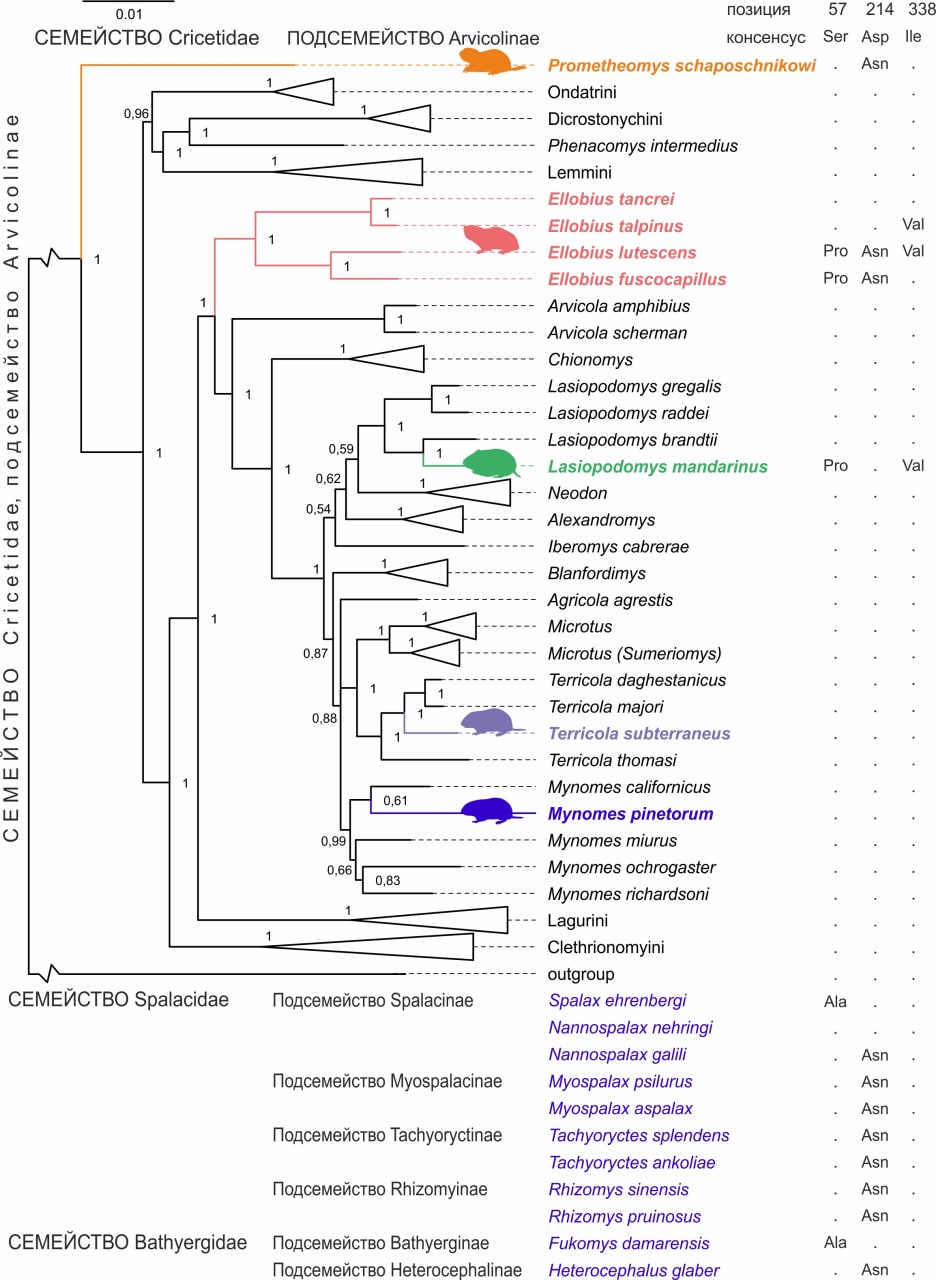
\includegraphics[width=0.68\textwidth]{Cytb_tree_colour_ed}
	\end{center}
	\caption{Филогенетическое дерево взятых в анализ видов. Указаны аминокислотные замены, характерные для подземных видов. Подземные виды отмечены цветом.}
	\label{PhyloTree}
\end{figure}

%\clearpage

\subsection{Оценка частоты несинонимичных замен}


Мы рассчитали распределение замен в каждом сайте \textit{CYTB} отдельно и объединили по координатам доменов. Анализ по сайтам показал три позиции (таблица \ref{CytB_sites}) с достоверно более высокими значениями частоты несинонимичных замен у подземных видов: 4, 237 и 241. Кроме того, в позиции 236 достоверно повышена частота синонимичных замен. Сравнение распределение замен по целым доменам (таблица \ref{CytB_domains}, рис. \ref{Cyt_Dom_fig}) выявило достоверные различия в уровне частот в мембранных доменах 1, 2, 5 и 9 и трансмембранных доменах 5 и 7 для несинонимичных замен (рис. \ref{Cyt_Dom_fig} A, рис. \ref{Cyt_Dom_str}); и мембранном домене 6 и трансмембранном домене 5 для синонимичных замен (рис. \ref{Cyt_Dom_fig} B). 


\begin{table}[h!]
	\caption{Сайты в гене \textit{CYTB} с достоверной разницей в частоте замен между подземными и наземными видами. NS -- несинонимичные замены, S -- синонимичные замены, Fs -- значения p.value при сравнении точным критерием Фишера, Holm -- значения p.value после поправки Холма-Бонферрони на множественные значения.}
	\label{CytB_sites}
	\vspace{5mm}
	
	\begin{center}
		\begin{tabular}{|c|c|c|c|c|c|}
			\hline 
			\textbf{Тип замен} & \textbf{Позиция} & \textbf{Подземные} & \textbf{Наземные} & \textbf{Fs} & \textbf{Holm} \\ \hline 
			NS & 4 & 0.875 & 0.1296 & 0.000049 & 0.023 \\ \hline 
			NS & 237 & 0.75 & 0.07 & 0.000084 & 0.038 \\ \hline 
			NS & 241 & 0.75 & 0.07 & 0.000084 & 0.039 \\ \hline 
			S & 236 & 1 & 0.148 & 0.0000038 & 0.002 \\ \hline 
		\end{tabular} 
	\end{center}
\end{table}

\begin{table}[h!]
	\caption{Домены в гене \textit{CYTB} с достоверной разницей в частоте замен между подземными и наземными видами. NS -- несинонимичные замены, S -- синонимичные замены, Fs -- значения p.value при сравнении точным критерием Фишера, Holm -- значения p.value после поправки Холма-Бонферрони на множественное тестирование, Memb -- мембранный домен, TM -- трансмембранный домен.}\label{CytB_domains}
	\vspace{5mm}
	\begin{center}	
		\begin{tabular}{|c|c|c|c|c|c|}
			\hline 
			\textbf{Домены} & \textbf{Подземные} & \textbf{Наземные} & \textbf{Тип замен} & \textbf{Fs} & \textbf{Holm}\\ \hline 
			Memb1 & 0.45 & 0.097 & NS & 0.00000033 & 0.000011\\ \hline 
			Memb2 & 0.33 & 0.043 & NS & 0.00001176 & 0.000365\\ \hline 
			Memb5 & 0.263 & 0.047 & NS & 0.00033176 & 0.008957\\ \hline 
			Memb9 & 0.52 & 0.15 & NS & 0.00005434 & 0.001522\\ \hline 
			TM5 & 0.64 & 0.10 & NS & 0.00000001 & 0.000000\\ \hline 
			TM7 & 0.29 & 0.06 & NS & 0.00004166 & 0.001208\\ \hline 
			Memb6 & 0.40 & 0.19 & S & 0.00000012 & 0.000004\\ \hline 
			TM5 & 0.42 & 0.19 & S & 0.00002733 & 0.000820 \\ \hline
		\end{tabular} 
	\end{center}
	
\end{table}

\begin{figure}[h!]
	\begin{center}
		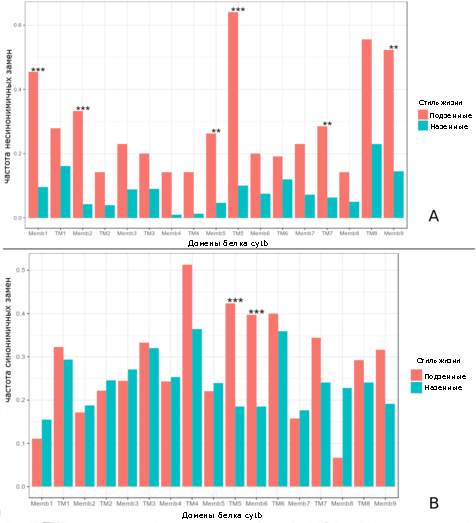
\includegraphics[width=0.7\textwidth]{cyt_domains}
	\end{center}
	\caption{Частоты распределения несинонимичных (A) и синонимичных (B) замен по доменам гена \textit{CYTB} у подземных и назменых грызунов. Достоверные различия обозначены звездочками(*): * -- p.value < 0,05, ** -- p.value < 0,01, *** -- p.value < 0,001. Memb -- мембранный домен, TM -- трансмембранный домен. }\label{Cyt_Dom_fig}
\end{figure}


\begin{figure}[h!]
	\begin{center}
		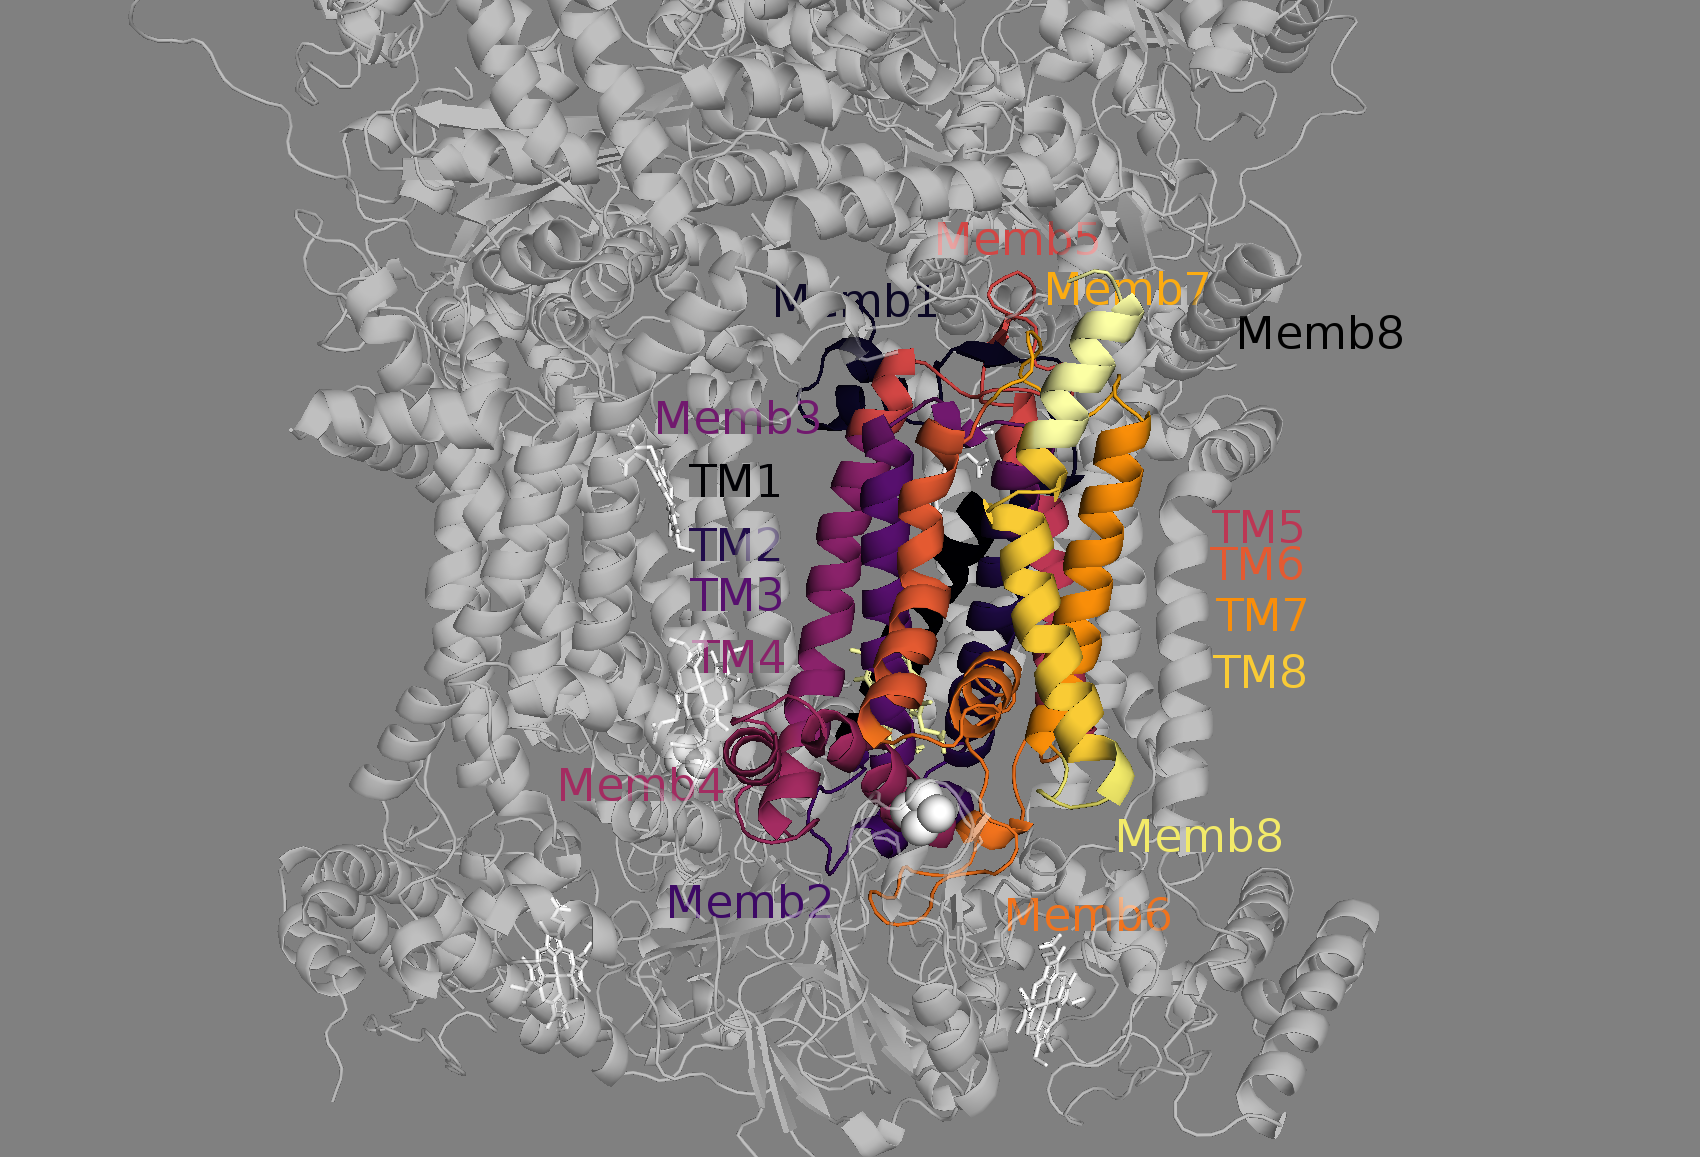
\includegraphics[width=0.5\textwidth]{tm_color}
	\end{center}
	\caption{Структурное положение доменов с достоверно повышенной частотой несинонимичных замен в белке цитохрома \textit{b}. Memb -- мембранный домен, TM -- трансмембранный домен. }\label{Cyt_Dom_str}
\end{figure}


\subsection{Поиск параллельных аминокислотных замен}

При анализе изменчивости гена \textit{CYTB} мы нашли три паралельные замены, характерные для подземных грызунов: Ser57Pro, Asp214Asn и Ile338Val (рис. \ref{PhyloTree}). Замена Asp214Asn была обнаружена также и у специализированных подземных грызунов из других семейств.

Замена серина на пролин в остатке 57 у подземных грызунов потенциально удаляет сайт фосфорилирования. Мы использовали два разных метода, чтобы оценить статус фосфорилирования этого сайта. Сервер NetPhos 3.1 предсказал фосфорилирование киназой \textit{CDC2} с оценкой 0,518. GPS 5.0 выявил киназы \textit{AGC}, \textit{PKN} и \textit{PKN1} с оценкой 65,363. Предсказания киназ не согласуются друг с другом, однако все прогнозы указывают на высокую вероятность фосфорилирования этого сайта. Те же методы не предсказывали фосфорилирование для Asp214Asn, и, насколько нам известно, ни Ile, ни Val в позиции 338 не могут быть фосфорилированы.

Нуклеотидная замена в кодоне 338 (ATT> GTT), приводящая к замене Ile338Val, была обнаружена как вероятный патоген в базе данных ClinVar и связана с раковыми процессами: www.ncbi.nlm.nih.gov/clinvar/variation/143898/.

Мы смоделировали третичную структуру белка цитохрома, чтобы изучить возможный структурный эффект замен (рис. \ref{CytStructure} A). Согласно ей, Ser57 обращен к межмембранному пространству митохондрий. Он расположен на неструктурированном сегменте петли, охватывающем остатки 54–60. Эта петля контактирует с той же петлей на втором мономере цитохрома \textit{bc1} в комплексе (рис. \ref{CytStructure} B). В отличие от Ser57Pro, замена Asp214Asn находится на петле, обращенной к матрице митохондрии. Он контактирует с N-концом субъединицы VII комплекса убихинол-цитохром с редуктазы III (UQCRQ) (рис. \ref{CytStructure} C). Замена Ile338Val находится на границе раздела $\alpha$-спиралей в трансмембранной области комплекса (рис. \ref{CytStructure} D). Смоделированная структура показывает, что эта замена благоприятствует другому ротамеру Ile350, который соседствует с остатком 58 UQCRQ.

\begin{figure}[h!]
	\begin{center}
		\includegraphics[width=0.8\textwidth]{fig структура}
	\end{center}
	\caption{Структурная модель замен в комплексе цитохрома \textit{bc1}. \textbf{A.} Обзор гомодимера цитохрома \textit{bc1}. Цитохром Б --- голубой, UQCRQ - пурпурный. Второй мономер окрашен в желтый цвет. Места замены выделены кружками. IMS --- межмембранное пространство. \textbf{B.} Увеличенные структуры \textit{E. lutescens} и \textit{L. sibiricus}, показывающие замену Ser57Pro. Модель \textit{E. lutescens} голубая, \textit{L. sibiricus} --- белая. \textbf{C.} Замена Asp214Asn и его взаимодействие с N-концом UQCRQ (пурпурный) \textbf{D.} Замена Ile338Val и соседняя цепочка UQCRQ (пурпурный).}
	\label{CytStructure}
\end{figure}

Для рассмотрения внутривидового аминокислотного полиморфизма в сайтах, выявленных программой TreeSAAP, был взят расширенный набор данных: 6 059 последовательностей \textit{CYTB} для наземных видов и 131 -- для подземных. Он включал в себя все, что было в базе данных GenBank по взятым в анализ видам на август 2020 года. Сравнение частот использования аминокислот в каждой позиции белка выявило более 60 сайтов с достоверными различиями между подземными и наземными видами (рис. \ref{Aa_sybst_structure}, Приложение Б). Среди них были обнаруженные в ходе анализа TreeSAAP позиции 57 и 338.

\begin{figure}[h!]
	\begin{center}
		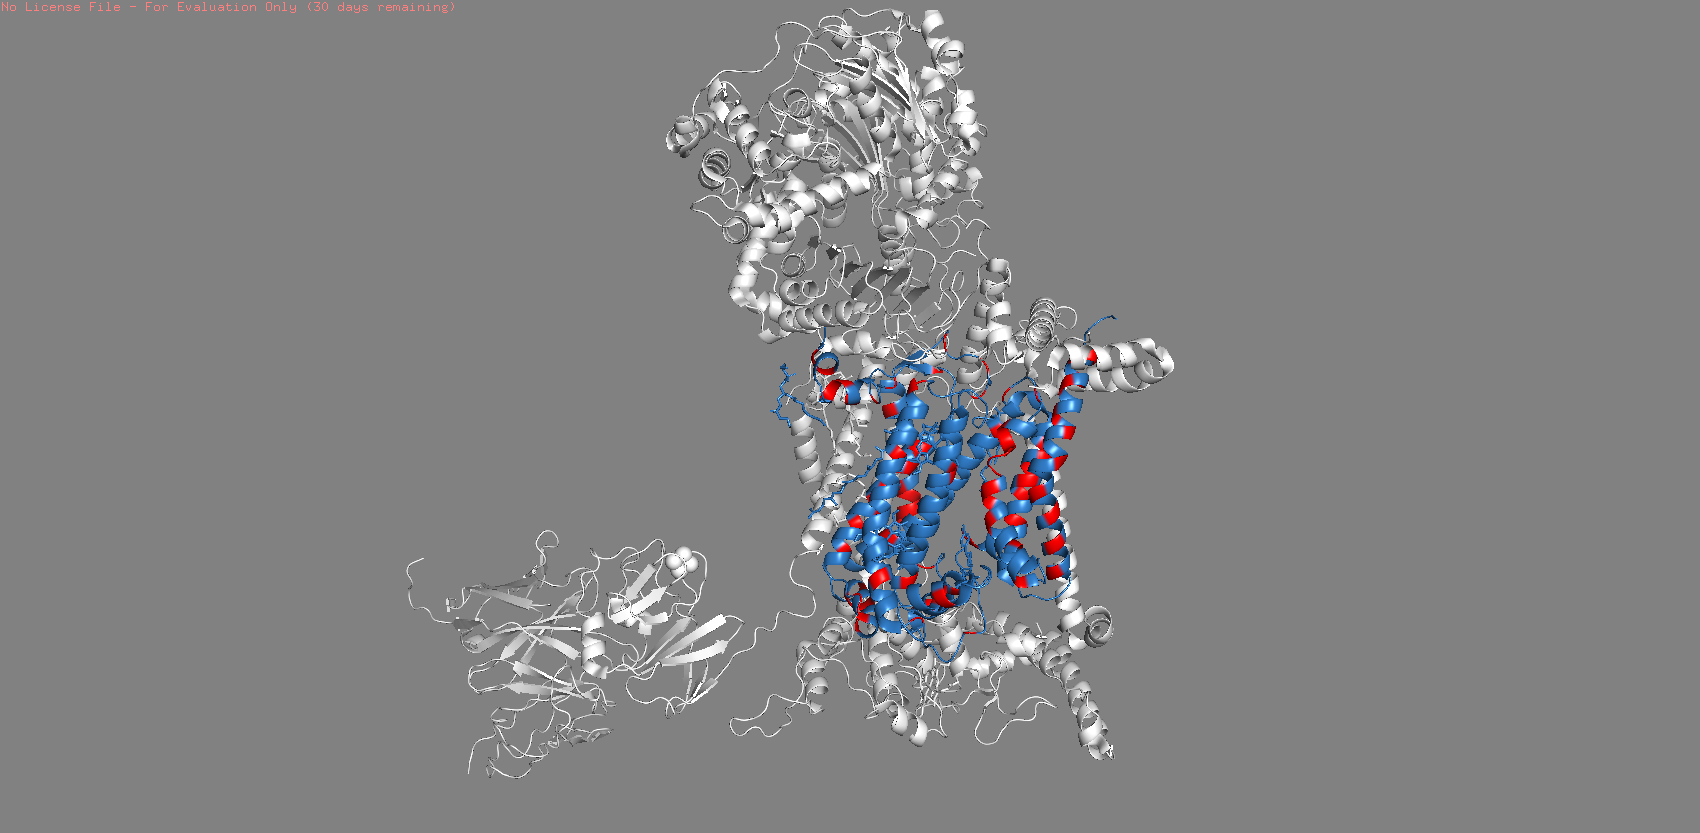
\includegraphics[width=0.9\textwidth]{aa_pattern_sites}
	\end{center}
	\caption{Структурная модель замен в белке цитохрома \textit{b}. Синим цветом отмечен белок цитохрома, красным --- сайты с достоверным отличием в частоте использования аминокислот у наземных и подземных грызунов.}
	\label{Aa_sybst_structure}
\end{figure}

\subsection{Оценка уровня отбора}
Оценка значений $\omega$ (отношение \textit{dN/dS}) у взятых в анализ видов показала общую тенденцию к ослаблению уровня отбора у подземных грызунов при сравнении их с филогенетически близкими наземными видами (рис. \ref{Tree4Selection})


\begin{figure}[h!]
	\begin{center}
		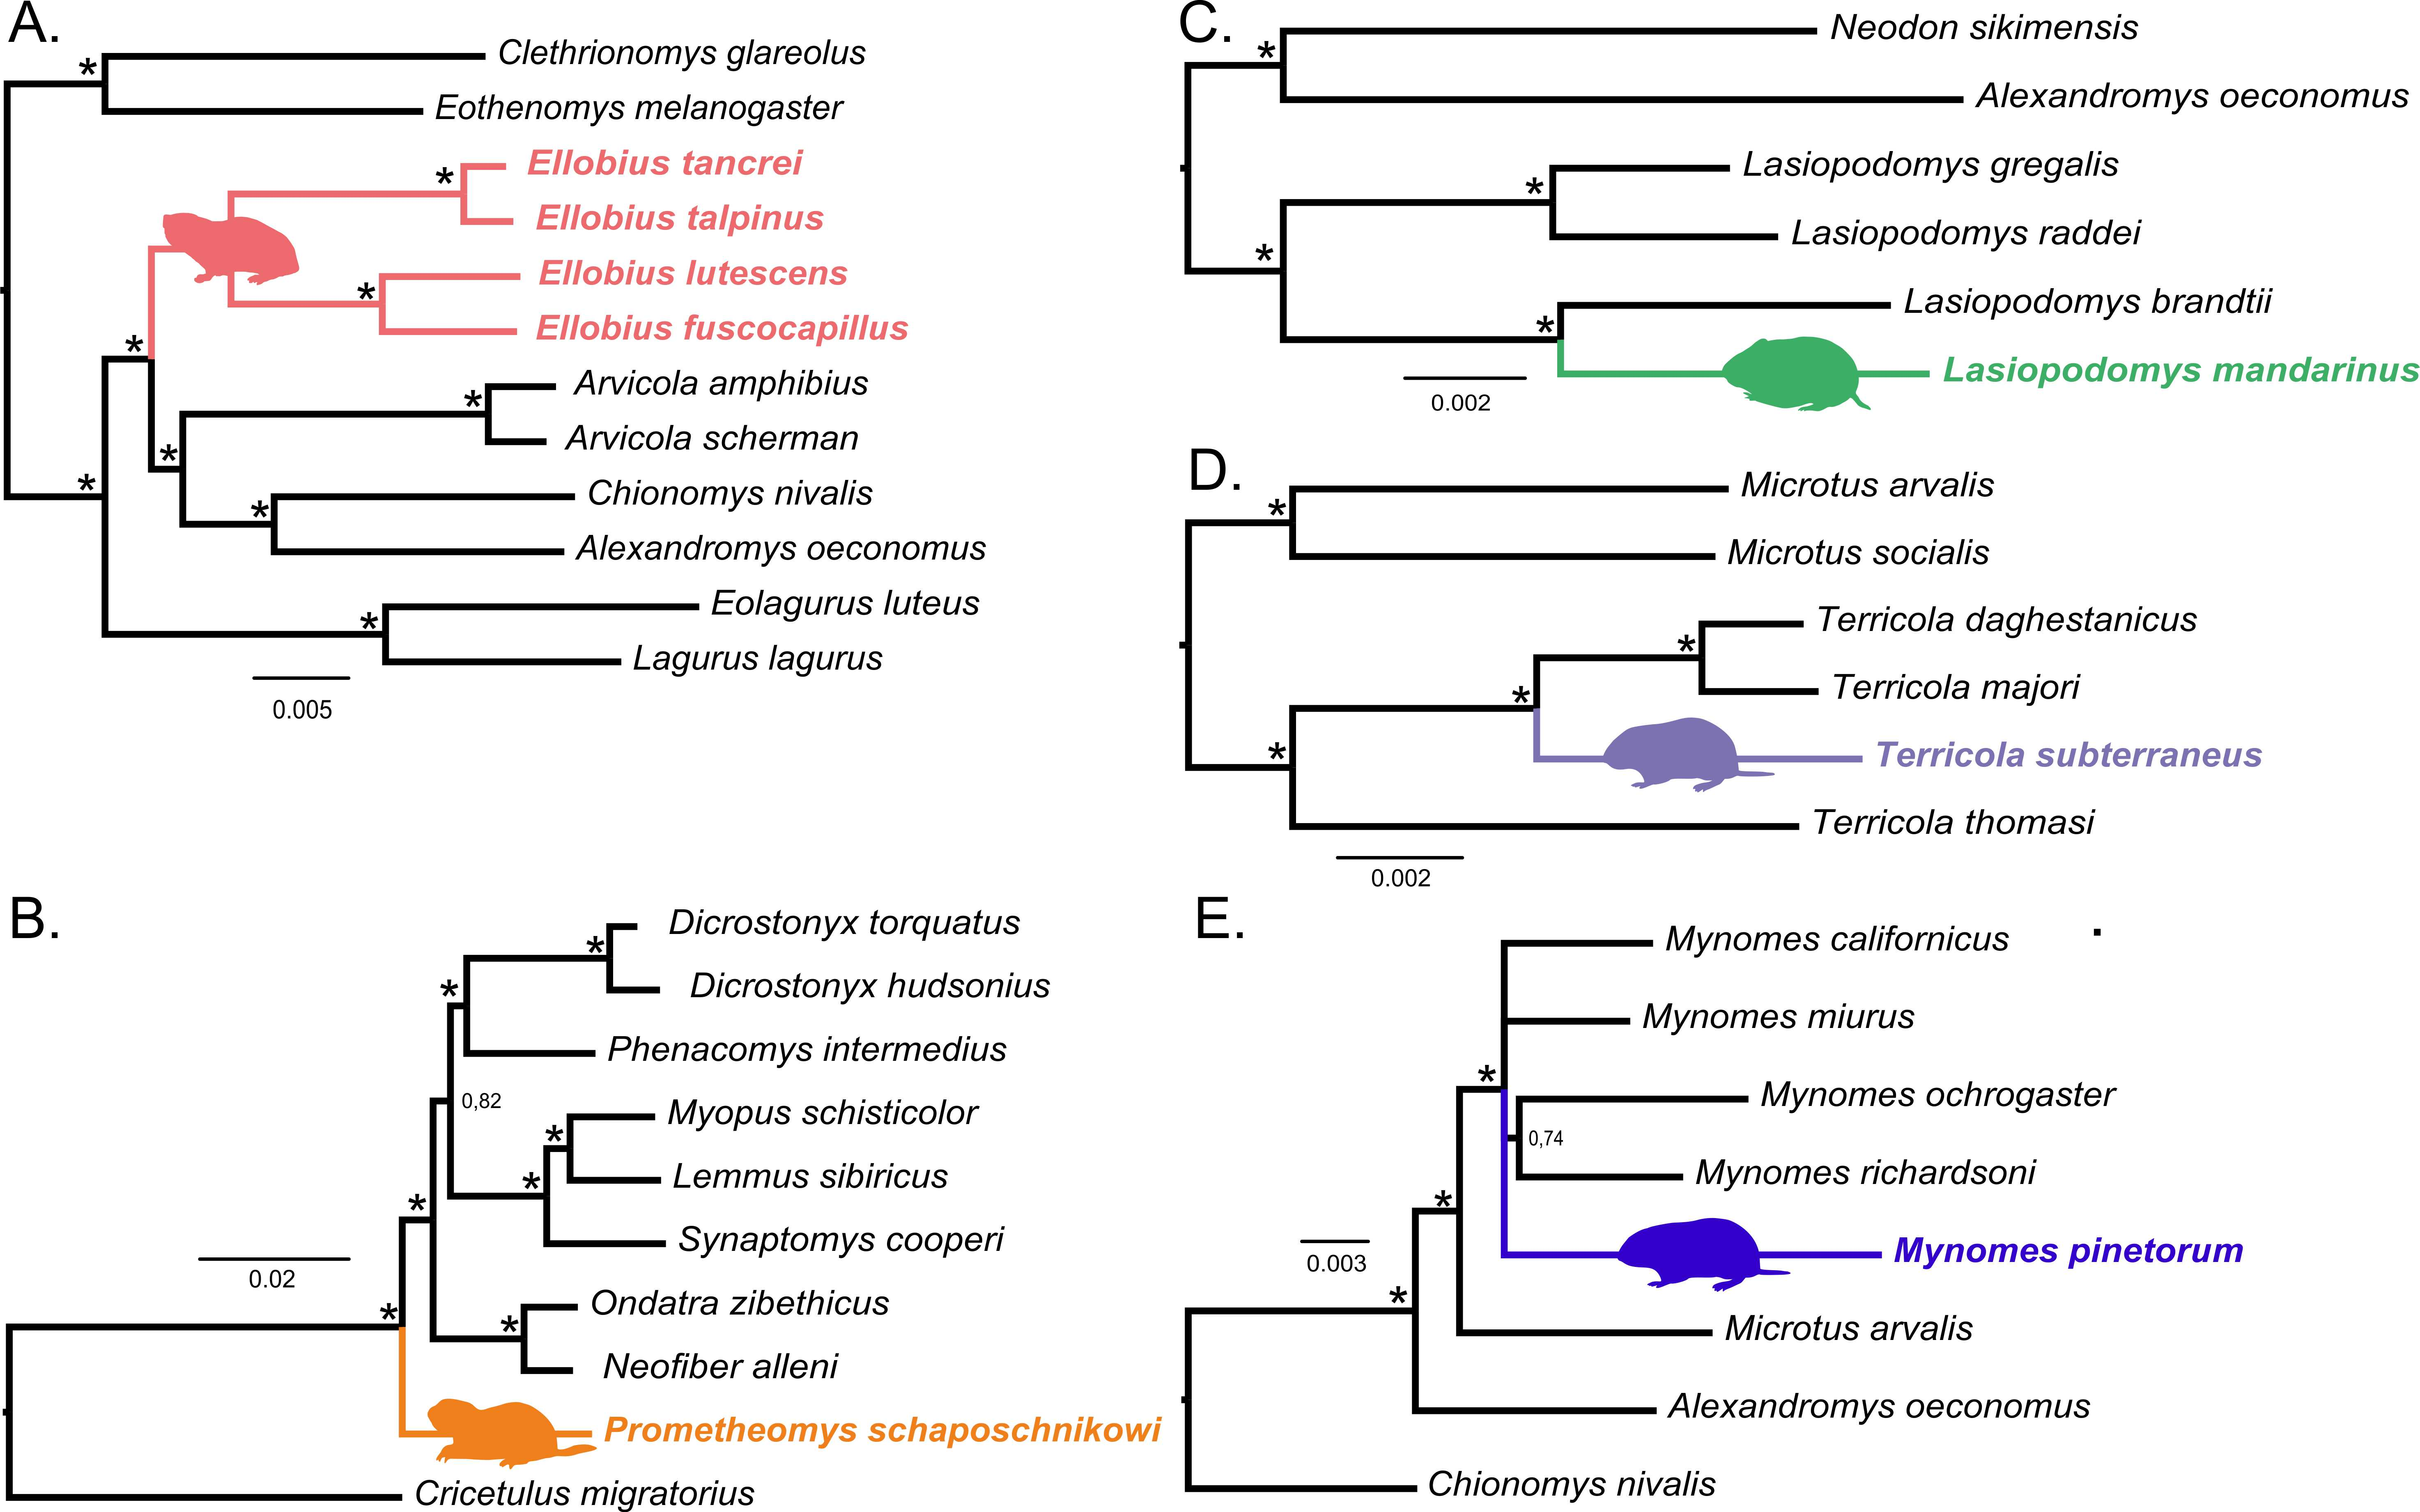
\includegraphics[width=\textwidth]{Cytb_separate_trees}
	\end{center}
	\caption{Филогенетические деревья, использованные для оценки отбора по отдельным ветвям. Подземные виды отмечены цветом. Звездочки (*) обозначают апостериорные байесовские вероятности 0,95 -- 1,0.} \label{Tree4Selection}
\end{figure}


 Достоверные отличия получены в результатах работы программы codeml для видов рода \textit{Ellobius}, \textit{Lasiopodomys mandarinus} и \textit{Terricola subterraneus}. Почти у всех подземных видов наблюдаются более высокие значения $\omega$ по сравнению наземными, за исключением \textit{T. subterraneus} (таблица \ref{PAMLtable}). Эта разница варьирует от одного (для \textit{Mymomes pinetorum}) до пяти раз для \textit{Lasiopodomys mandarinus}. Тесты сравнения с нейтральной моделью (b\_neut, таблица \ref{PAMLtable}) показали, что нуклеотидные последовательности гена \textit{CYTB} эволюционно не нейтральны у всех подземных грызунов. 

Анализ алгоритмом aBSREL не показал свидетельств эпизодического отбора в анализируемой филогении. Результаты программы RELAX подтвердили изменения в уровне естественного отбора у подземных грызунов. Так, коэффициент отбора K для трех подземных представителей (\textit{Ellobius sp.}, \textit{L. mandarinus} и \textit{P. schaposchnikowi}; таблица \ref{Relax_cyt}) показал значения < 1, что может указывать на ослабление уровня отбора. В то же время, для представителей рода \textit{Ellobius} и для \textit{L. mandarinus} показаны повышенные значения $\omega$ при анализе отбора методом codeml. Значение K для \textit{T. subterraneus} намного превышало 1, что можно интерпретировать как то, что сила отбора увеличилась и коррелировала с более низким значением $\omega$ по сравнению с видами, обитающими на поверхности. Суммируя результаты этих анализов, можно сказать о наличии следов ослабления отбора в гене \textit{CYTB} у почти всех подземных грызунов.


\begin{table}[h!]
	\caption{Оценка $\omega$ с использованием branch model codeml. Fg --- foreground branch (подземные виды), Bg --- background branch (наземные виды). Подземные виды обозначены цветом на рисунке \ref{Tree4Selection}. b\_free --- модель независимого расчета по ветвям, b\_neut --- нейтральная модель. Достоверность сравнения типов моделей выражена в p.value, достоверные значения отмечены \textbf{жирным}.}\label{PAMLtable}
	\vspace{5mm}
	
\begin{center}
\begin{tabular}{|c|c|c|p{4.5cm}|p{4.5cm}|}
	\hline 
\textbf{Подземные виды} & \textbf{Fg} & \textbf{Bg} & \textbf{Сравнение моделей b\_free и M0} & \textbf{Сравнение моделей b\_free и b\_neut}\\ \hline
\textit{Ellobius sp.} & \textbf{0.0642} & \textbf{0.0243} & \textbf{2.33E-06} & \textbf{4.76E-81}\\ \hline
\textit{L. mandarinus} & \textbf{0.1325} & \textbf{0.0269} & \textbf{4.69E-05} & \textbf{0.00024}\\ \hline
\textit{M. pinetorum} & 0.0233 & 0.0224 & 0.9327 & \textbf{4.62E-24}\\ \hline
\textit{P. schaposchnikowi} & 0.0617 & 0.0356 & 0.0711 & \textbf{1.26E-09}\\ \hline
\textit{T. subterraneus} & \textbf{0.0071} & \textbf{0.0343} & \textbf{0.05} & \textbf{2.48E-17}\\ \hline
\end{tabular} 
\end{center}
\end{table}

%\clearpage

\begin{table}[h!]
	\caption{Оценка уровеня отбора с использованием программы RELAX. K --- значение коэффициента отбора, P --- p-value, LRT --- likelihood ratio test. Подземные виды обозначены цветом на рисунке \ref{Tree4Selection}. Достоверные результаты отмечены \textbf{жирным}.}\label{Relax_cyt}
	\vspace{5mm}
	
\begin{center}
	\begin{tabular}{|c|l|l|l|}
		\hline
		\textbf{}                     & \multicolumn{3}{c|}{RELAX}              \\ \hline
		\textbf{Подземные виды} & \textbf{K}     & \textbf{P}     & \textbf{LRT}   \\ \hline
		\textit{Ellobius sp.}         & \textbf{0.52}  & \textbf{0}     & \textbf{23.97} \\ \hline
		\textit{L. mandarinus}        & \textbf{0}     & \textbf{0.001} & \textbf{11.78} \\ \hline
		\textit{M. pinetorum}         & 1.05           & 0.804          & 0.06           \\ \hline
		\textit{P. schaposchnikowi}   & \textbf{0.63}  & \textbf{0.023} & \textbf{5.15}  \\ \hline
		\textit{T. subterraneus}      & \textbf{23.22} & \textbf{0.014} & \textbf{6.02}  \\ \hline
	\end{tabular}
\end{center}
\end{table}


%\clearpage

\section{Поиск следов отбора в митохондриальных геномах}

\subsection{Характеристика собранных митохондриальных геномов}

Всего в лаборатории эволюционной геномики и палеогеномики ЗИН РАН было собрано 34 новых митохондриальных генома представителей Arvicolinae (Приложение В). Все собранные последовательности, а также доступные в базе данных GenBank, были использованы для реконструкции филогении подсемейства.


%Наземные виды: \textit{Ondatra zibethicus} Linnaeus, 1766; \textit{Dicrostonyx torquatus} Pallas, 1778; \textit{Myopus schisticolor} Lilljeborg, 1844; \textit{Lemmus sibiricus} Kerr, 1792; \textit{Alticola tuvinicus} Ognev, 1950; \textit{Alticola strelzovi} Kastsch, 1899; \textit{Craseomys rufocanus} Sundevall, 1846; \textit{Craseomys regulus} Thomas, 1906; \textit{Clethrionomys glareolus} Schreber, 1780; \textit{Lasiopodomys brandtii} Radde, 1861; \textit{Lasiopodomys gregalis} Pallas, 1779; \textit{Alexandromys fortis} Büchner, 1889; \textit{Chionomys nivalis} Martins, 1842; \textit{Chionomys gud} Satunin, 1909; \textit{Lagurus lagurus} Pallas, 1773; \textit{Eolagurus luteus} Eversmann, 1840; \textit{Microtus californicus} Peale, 1848; \textit{Microtus longicaudus} Merriam, 1888; \textit{Microtus arvalis} Pallas, 1778; \textit{Microtus socialis} Pallas, 1773; \textit{Terricola daghestanicus} Shidlovsky, 1919.

%Подземные виды: \textit{Prometheomys shchaposhnikowi}, \textit{Lasiopodomys mandarinus}, \textit{Ellobius} (4 вида), \textit{Terriocola subterraneus}, \textit{Hyperacrius fertilis} True, 1894.

Отдельной задачей была проверка качества ридов для \textit{Hyperacrius fertilis} из-за древности образца (1903 г.). Молекуляное изучение музейных коллекций требует множества дополнительных проверок качества сырых прочтений. Прежде всего, из-за проблемы дезаминирования, которая возникает в виде включения тимина вместо цитозина (C-to-T) на 5'-концах и аденина вместо гуанина (G-to-A) на 3'-концах последовательности. Анализ программой mapDamage показал низкое значение дезаминирования (рис. \ref{MapDamage}). Неправильное включение тимина вместо цитозина (красный) варьировалось от 12.09 \% до 17.94 \%, аденина вместо гуанина (синий) -- от 12.84 \% до 17.49 \%. Уровни ошибочного включения сравнимы со всеми другими вариантами замен, окрашенными в серый цвет, а также аналогичными значениям из статей (\cite{Molto2017}), что позволило взять образец в дальнейший анализ. 


\begin{figure}[h!]
	\begin{center}
		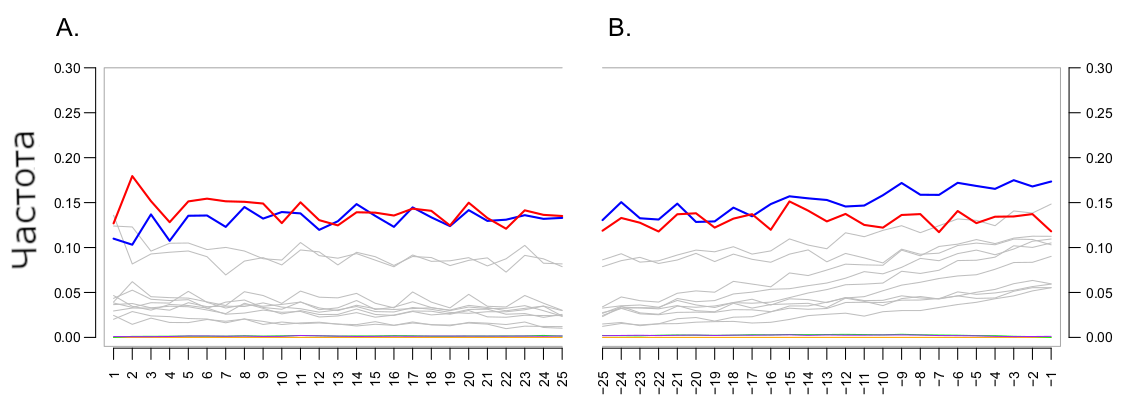
\includegraphics[width=\textwidth]{MapDamage Hyper}
	\end{center}
	\caption{Замены, которые могут являться следствием дезаминирования нуклеотидов, помечены цветом: замены гуанина на аденин (G > A, голубой цвет) и цитозина на тимин (C > T, красный цвет). Остальные варианты замен отмечены серым.}\label{MapDamage}
\end{figure}


Собранные митогеномы представляют собой кольцевые двуцепочечные последовательности ДНК (рис. \ref{mitogenome}). Состав и порядок генов всех последовательностей соответствует структуре митохондриального генома других млекопитающих: 13 белок-кодирующих генов, 22 транспортные РНК (тРНК), две рибосомные РНК (рРНК) и некодирующая регуляторная область (D-петля). Девять генов (\textit{ND6} и 8 тРНК) были ориентированы в обратном (reverse) направлении, тогда как остальные транскрибировались в прямом. Нами не было обнаружено каких-либо структурных изменений в порядке генов или их количестве, которые отличали бы подземных грызунов от наземных сестринских видов.

\begin{figure}[h!]
	\begin{center}
		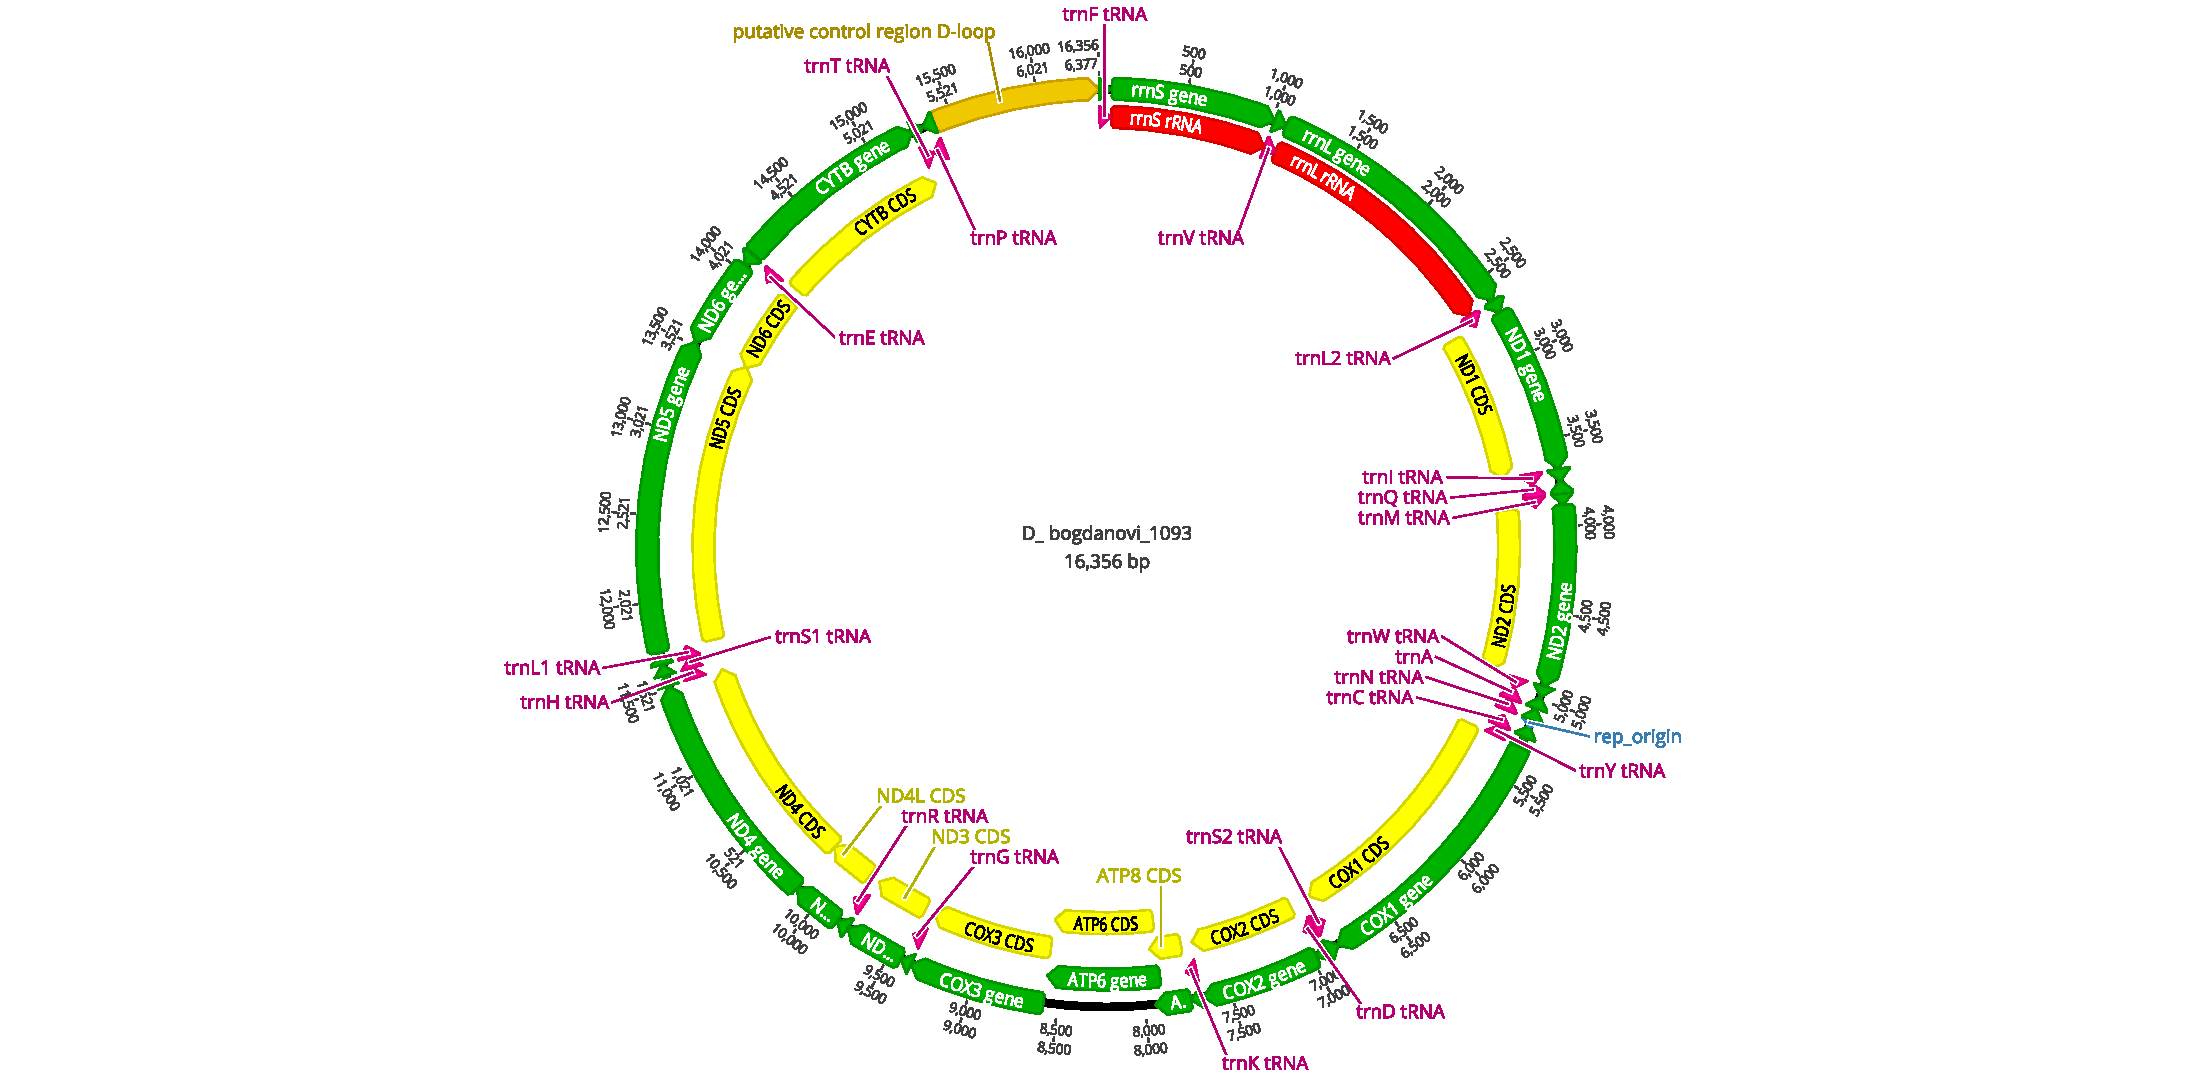
\includegraphics[width=\textwidth]{Dinaromys_mitogenome}
	\end{center}
	\caption{Собранный митохондриальный геном \textit{Dinaromys bogdanovi} Martino, 1922. Зеленым отмечены гены, желтым -- CDS, красным -- рРНК, розовым -- тРНК}\label{mitogenome}
\end{figure}

Филогенетическая реконструкция (рис. \ref{Tree_13_genes}) с использованием митохондриальных геномов полевочьих на полноценной выборке таксонов в целом не противоречит предыдущим данным Абрамсон Н.И. с соавторами (\cite{Abramson2009}).  

\begin{figure}[h!]
\begin{center}
	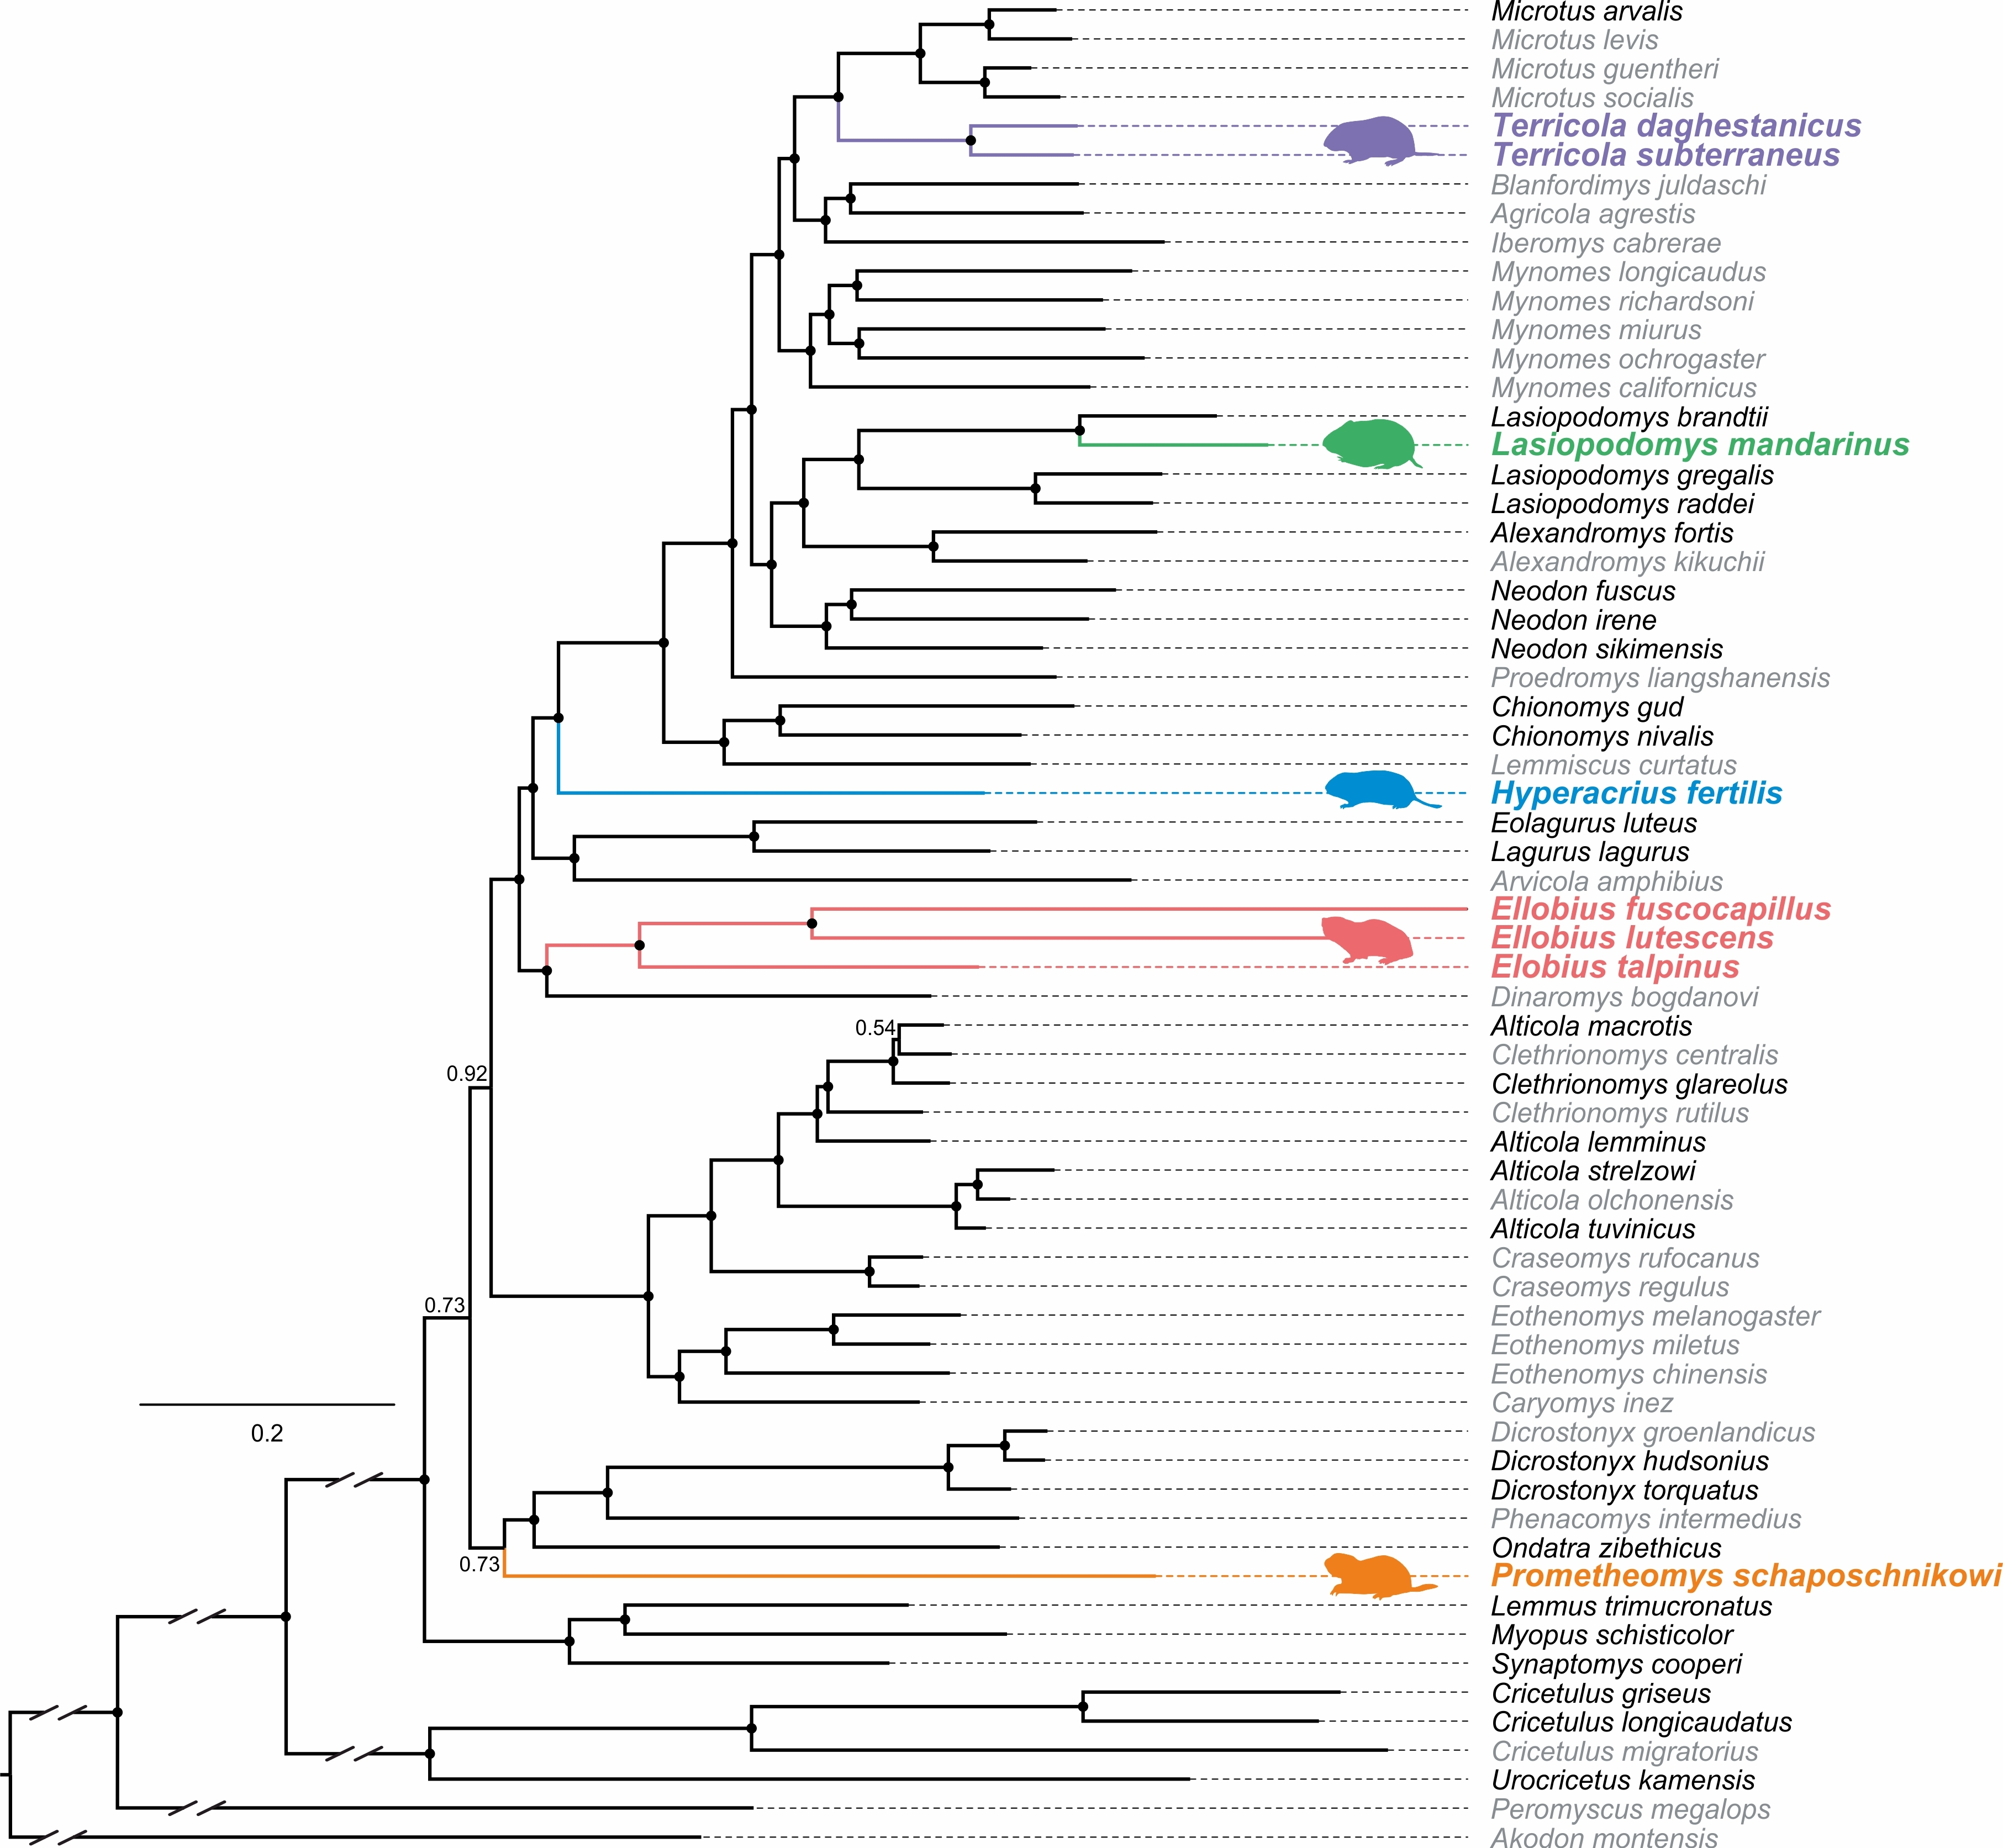
\includegraphics[width=\textwidth]{main_tree_mito_col}
\end{center}
	\caption{Филогенетическое дерево, построенное по последовательности 13 белок-кодирующих генов. Подземные виды обозначены цветом.}
	\label{Tree_13_genes}
\end{figure}


Для начала мы сравнили митохондриальные геномы по GC-обогащенности и смещению нуклеотидов в паре GC (GC-skew). Результаты сравнения показали увеличение среднего значения \% GC и уменьшение GC-skew. Разница в различиях оказалась недостоверная (рис. \ref{boxplot_GC_GSskew}). 

\begin{figure}[h!]
\begin{center}
	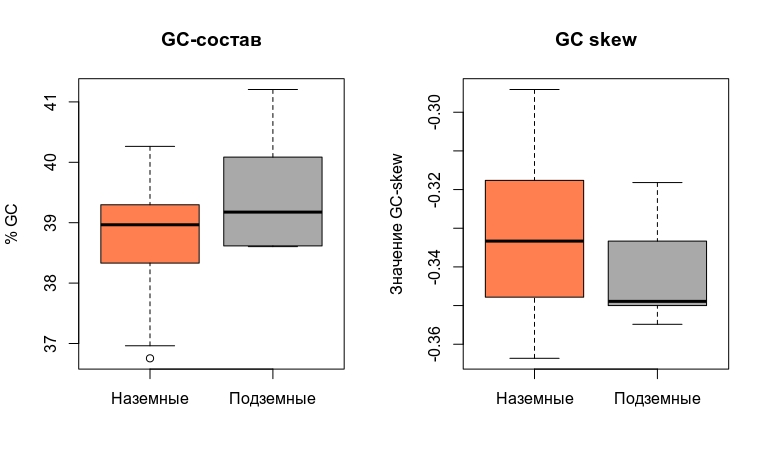
\includegraphics[width=0.7\textwidth]{GC genomes}
\end{center}
\caption{Сравнение \% GC и GC-skew у подземных и наземных видов}\label{boxplot_GC_GSskew}
\end{figure}


\subsection{Анализ частоты несинонимичных замен}

При подсчете количества несинонимичных замен и нормировке их на количество взятых в анализ видов (рис. \ref{boxplot_NS}) оказалось, что доля замен в митохондриальных геномах подземных грызунов достоверно выше, чем у наземных.  При оценке частот замен по каждому белок-кодирующему гену в отдельности тенденция повторяется --- в каждом гене доля несинонимичных замен достоверно выше у подземных грызунов, чем у наземных (табл. \ref{ns_by_genes}).

\begin{figure}[h!]
\begin{center}
	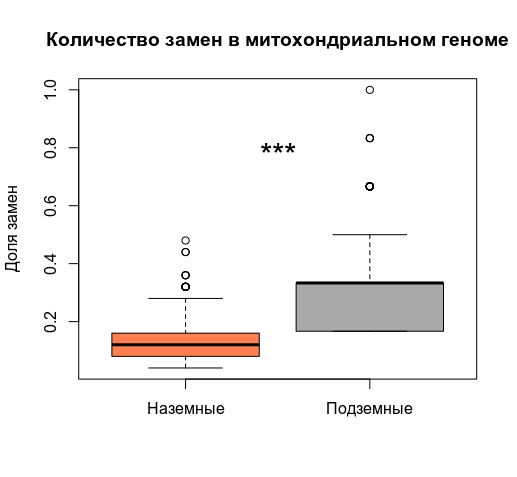
\includegraphics[width=0.6\textwidth]{Subst_all_boxplot}
\end{center}
	\caption{Соотношение несинонимичных замен у наземных и подземных грызунов}\label{boxplot_NS}
\end{figure}


%\begin{figure}[h!]
%	\begin{center}
%		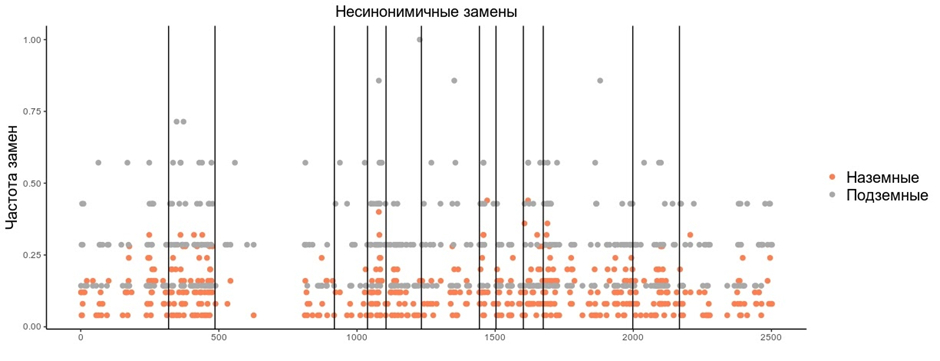
\includegraphics[width=0.9\textwidth]{Distribution_mitogenomes}
%	\end{center}
%	\caption{Распределение несинонимичных замен по белок-кодирующим генам у подземных и наземных грызунов.}\label{manhattan_NS}
%\end{figure}

\begin{table}[h!]
		\caption{Частота несинонимичных замен в митохондриальных генах. p.value -- значения p.value при сравнении точным критерием Фишера, Holm -- значения p.value после поправки Холма-Бонферрони на множественное тестирование.}\label{ns_by_genes}
	\vspace{5mm}
	\begin{tabular}{|l|l|l|l|l|}
		\hline
		\textbf{Ген} & \textbf{Наземные} & \textbf{Подземные} & \textbf{p.value} & \textbf{Holm} \\ \hline
		\textit{ATP6} & 0.099 & 0.253 & 0.000000040 & 0.000000317 \\ \hline
		\textit{ATP8} & 0.133 & 0.355 & 0.000000134 & 0.000000940 \\ \hline
		\textit{COX1} & 0.094 & 0.253 & 0.000021490 & 0.000107451 \\ \hline
		\textit{COX2} & 0.088 & 0.297 & 0.000188734 & 0.000566201 \\ \hline
		\textit{COX3} & 0.111 & 0.296 & 0.000000464 & 0.000002782 \\ \hline
		\textit{CYTB} & 0.097 & 0.262 & 0.000000000 & 0.000000000 \\ \hline
		\textit{ND1} & 0.121 & 0.252 & 0.000000020 & 0.000000200 \\ \hline
		\textit{ND2} & 0.136 & 0.299 & 0.000000000 & 0.000000000 \\ \hline
		\textit{ND3} & 0.155 & 0.313 & 0.000889496 & 0.001778992 \\ \hline
		\textit{ND4} & 0.149 & 0.260 & 0.001607514 & 0.001778992 \\ \hline
		\textit{ND4L} & 0.098 & 0.197 & 0.000061623 & 0.000246493 \\ \hline
		\textit{ND5} & 0.124 & 0.278 & 0.000000000 & 0.000000000 \\ \hline
		\textit{ND6} & 0.111 & 0.260 & 0.000000023 & 0.000000208 \\ \hline
	\end{tabular}
\end{table}


\subsection{Поиск параллельных аминокислотных замен}

Мы, по аналогии с логикой исследования гена \textit{CYTB}, искали характерные только для подземных грызунов паралелльные аминокислотные замены. При анализе белок-кодирующих митохондриальных генов были выявлены замены в генах \textit{COX1, COX3, ND5, ND6} и \textit{CYTB} (таблица \ref{Underground_subs}). Больше всего замен было обнаружено в гене \textit{CYTB}. При дальнейшей проверке оказалось, что вероятность этих замен не достоверные.

\begin{table}[h!]
	\caption{Обнаруженные параллельные аминокислотные замены у подземных грызунов.}\label{Underground_subs}
	\vspace{5mm}
\begin{tabular}{|l|c|c|c|c|c|c|}
	\hline
	& \textit{COX1} & \textit{COX3} & \textit{ND5} & \multicolumn{3}{c|}{\textit{CYTB}} \\ \hline
	Вид   / позиция              & 73   & 121  & 466 & 56      & 338    & 357    \\ \hline
	Наземные виды                & Met  & Ile  & Phe & Thr     & Ile    & Ala    \\ \hline
	\textit{Ellobius lutescens}          & Val  & --   & --  & Ser     & Val    & --     \\ \hline
	\textit{Ellobius fuscocapillus}       & Ile  & --   & Leu & --      & --     & Thr    \\ \hline
	\textit{Ellobius talpinus}            & --   & Val  & Leu & --      & Val    & --     \\ \hline
	\textit{Prometheomys schaposchnikowi} & Ile  & Val  & --  & Ser     & --     & Thr    \\ \hline
	\textit{Lasiopodomys mandarinus}      & Ile  & --   & --  & Ser     & Val    & Thr    \\ \hline
	\textit{Hyperacrius fertilis}         & --   & Val  & --  & --      & --     & --     \\ \hline
	\textit{Terricola subterraneus}       & --   & --   & Leu & --      & --     & --     \\ \hline
\end{tabular}	
\end{table}


\subsection{Оценка уровня и направления отбора}

Уровень и направление отбора на белок-кодирующих генах оценивали отдельно по каждому подземному виду (или нескольким в случае рода \textit{Ellobius}), сравнивая его только с филогенетически близкими наземными видами (рис. \ref{tree_mito}) несколькими подходами: REXAL, aBSREL и codeml. Из-за базального положения \textit{P. schaposchnikowi} уровень отбора оценивали дважды, сравнивания его с хомяками и с другими представителями <<первой>> радиации.   

\begin{figure}[h!]
	\begin{center}
		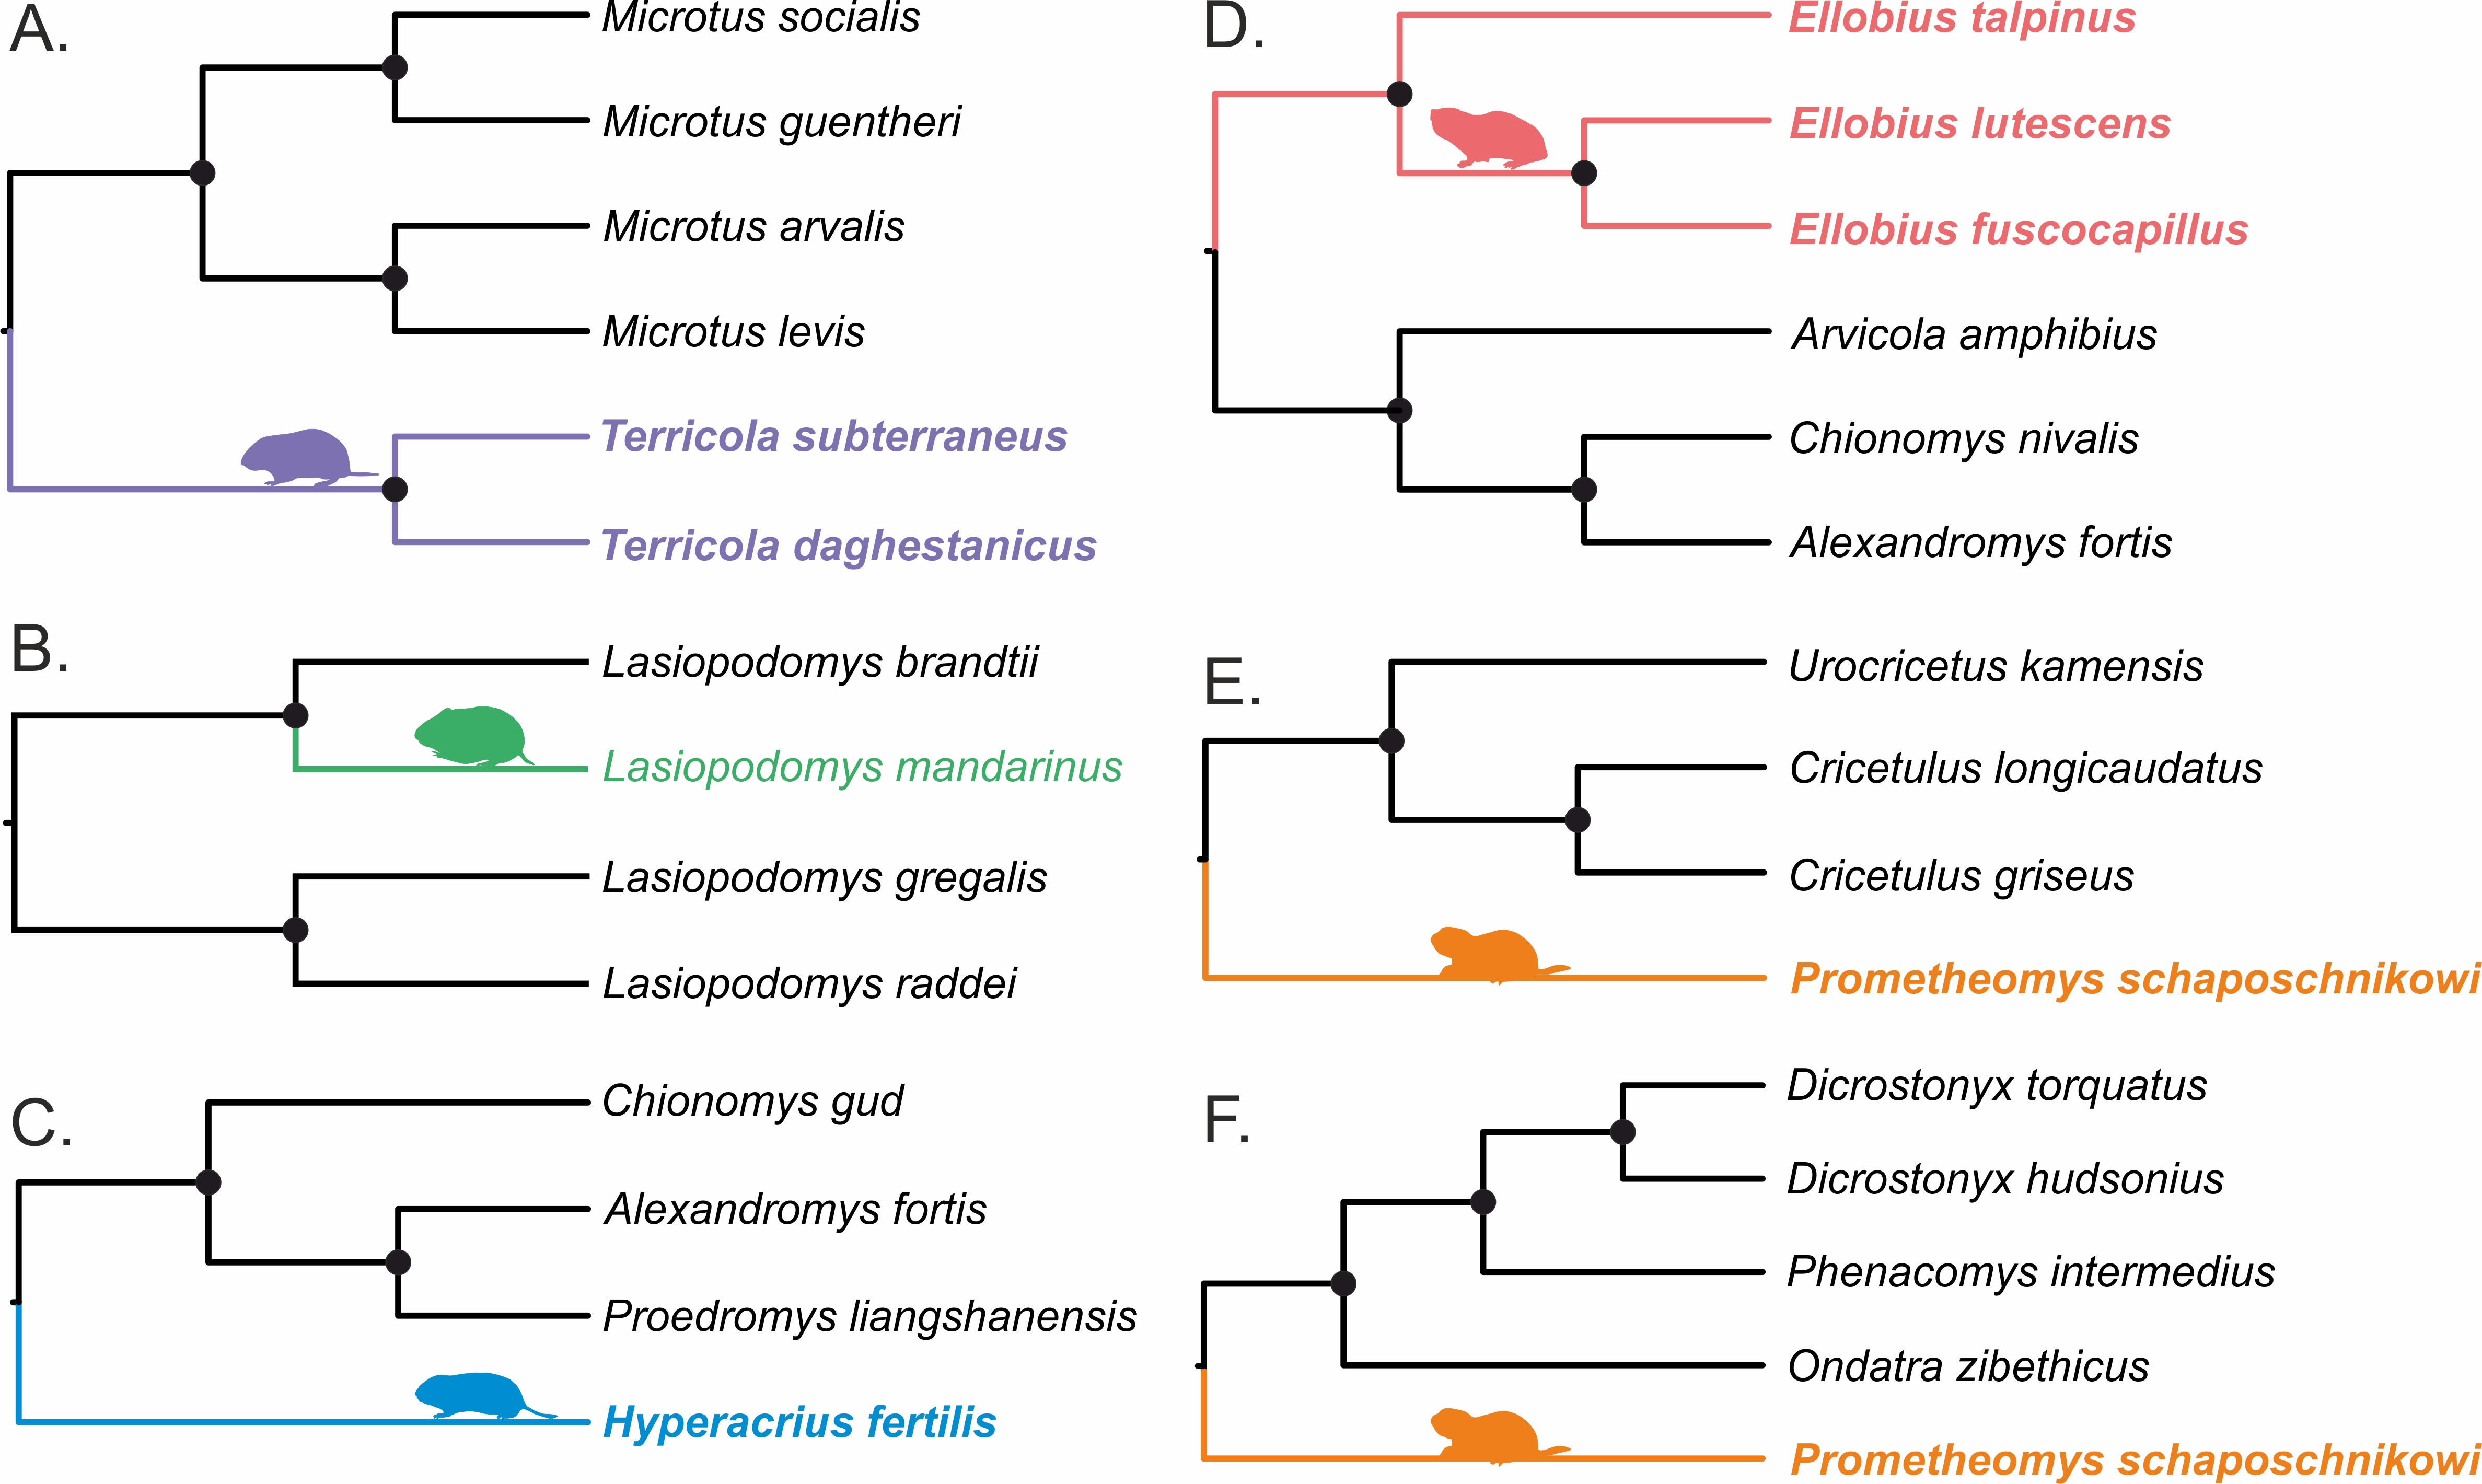
\includegraphics[width=\textwidth]{separate_mito_col}
	\end{center}
	\caption{Филогенетические деревья, использованные для оценки отбора отдельных ветвей. Подземные виды обозначены цветом. Для каждого подземного вида или группы видов использовались филогенетически близкие наземные таксоны.}
	\label{tree_mito}
\end{figure}


Для каждого из подземных грызунов мы провели сравнение по каждому митохондриальному гену (таблица \ref{MT_branch}). У представителей рода \textit{Ellobius} при оценке  codeml разница в отборе наблюдается во всех митохондриальных генах, кроме \textit{ND2, 3, 5, 6} и \textit{COX3}. Несколько генов под отбором обнаружено также у \textit{L. mandarinus}: \textit{COX3} и \textit{CYTB}. Только один ген с достоверной разницей в уровне отбора найден для \textit{P. schaposchnikowi} --- \textit{COX3}. У оставшихся представителей подземных грызунов не обнаружено генов с достоверным отличием от наземных видов. Значимые различия наблюдались в последовательностях \textit{COX3} и \textit{CYTB} для двух подземных видов одновременно: в \textit{COX3} для \textit{P. schaposchnikowi} и \textit{L. mandarinus} и в \textit{CYTB} для \textit{L. mandarinus} и представителей рода \textit{Ellobius}. 
Хотя значения $\omega$ существенно различались в зависимости от генов и анализируемых видов, в любом случае оно не превышало единицы. Однако все достоверно различающиеся значения $\omega$ были выше для подземных видов, чем для наземных. 

\begin{landscape}
	
	\begin{table}[]
		\caption{Оценка уровня отбора независимо у всех филогенетических линий подземных грызунов методом codeml. \textbf{Жирным} обозначены достоверные различия между подземными и наземными видами после поравки на множественное сравнение. Fg --- foreground branch (подземные виды), Bg --- background branch (наземные виды). Ветви обозначены цветом на рисунке \ref{tree_mito}. NA -- рассчитать значение невозможно. }\label{MT_branch} \vspace{5mm}
		\large
		
		\begin{tabular}{|c|c|c|c|c|c|c|c|c|c|c|c|c|}
			\hline
			\multicolumn{1}{|l|}{}    & \multicolumn{2}{l|}{\textit{Ellobius sp.}} & \multicolumn{2}{p{5cm}|}{\textit{P. schaposchnikowi \& \textit{Cricetulus sp.}}} & \multicolumn{2}{p{5cm}|}{\textit{P. schaposchnikowi \& первая радиация}} & \multicolumn{2}{l|}{\textit{L. mandarinus}} & \multicolumn{2}{l|}{\textit{H. fertilis}} & \multicolumn{2}{l|}{\textit{Terricola}} \\ \hline
			\multicolumn{1}{|l|}{Ген} & fg & bg & fg & bg & fg & bg & fg & bg & fg & bg & fg & bg \\ \hline
			{\textit{ATP6}} & \textbf{0.132} & \textbf{0.039} & NA & 0.015 & NA & 0.034 & 0.138 & 0.075 & NA & 0.022 & 0.042 & 0.030 \\ \hline
			\textit{ATP8} & \textbf{0.739} & \textbf{0.163} & 0.903 & 0.153 & 0.376 & 0.269 & 0.184 & 0.240 & NA & 0.198 & 0.095& 0.079 \\ \hline
			\textit{COX1} & \textbf{0.033} & \textbf{0.009} & 0.138 & 0.008 & 0.029 & 0.010 & 0.036 & 0.023 & NA & 0.007 & 0.002& 0.027 \\ \hline
			\textit{COX2} & \textbf{0.217} & \textbf{0.022} & NA & 0.006 & 0.023 & 0.029 & 0.108 & 0.039 & NA & 0.018 & 0.030& 0.029 \\ \hline
			\textit{COX3} & 0.087 & 0.044 & \textbf{0.051} & \textbf{0.012} & 0.055 & 0.019 & \textbf{0.117} & \textbf{0.028} & NA & 0.033 & 0.028& 0.041 \\ \hline
			\textit{CYTB} & \textbf{0.060} & \textbf{0.021} & 0.048 & 0.021 & 0.050 & 0.028 & \textbf{0.234} & \textbf{0.028} & NA & 0.021 & 0.017& 0.030 \\ \hline
			\textit{ND1} & \textbf{0.064} & \textbf{0.029} & 0.042 & 0.030 & 0.059 & 0.021 & 0.075 & 0.020 & 0.009 & 0.027 & 0.011& 0.035 \\ \hline
			{\textit{ND2}} & 0.133 & 0.084 & NA & 0.048 & NA & 0.085 & 0.198 & 0.085 & NA & 0.076 & 0.104& 0.092 \\ \hline
			\textit{ND3} & 0.119 & 0.057 & 0.063 & 0.027 & NA & 0.067 & 0.234 & 0.116 & NA & 0.019 & 0.079& 0.094 \\ \hline
			\textit{ND4} & \textbf{0.095} & \textbf{0.045} & 0.045 & 0.031 & 0.095 & 0.057 & 0.165 & 0.072 & 0.107 & 0.051 & 0.035& 0.075 \\ \hline
			\textit{ND4L} & \textbf{0.179} & \textbf{0.038} & 0.009 & 0.017 & NA & 0.101 & 0.100 & 0.073 & NA & 0.036 & 0.000& 0.083 \\ \hline
			{\textit{ND5}} & 0.098 & 0.069 & 0.071 & 0.037 & NA & 0.052 & 0.179 & 0.068 & NA & 0.062 & 0.093& 0.055 \\ \hline
			\textit{ND6} & 0.149 & 0.084 & NA & 0.052 & 0.681 & 0.045 & 0.054 & 0.121 & NA & 0.104 & 0.013& 0.046 \\ \hline
			
		\end{tabular}
	\end{table}

\end{landscape}

Используя алгоритм aBSREL, мы обнаружили следы эпизодического положительного отбора в гене \textit{COX2} для \textit{E. lutescens} и в двух генах \textit{P. schaposchnikowi}: \textit{ATP8} при сравнении с видами Arvicolinae и \textit{ND5} при сравнении с хомяками (таблица \ref{MT_absrel}).

\begin{table}[h!]
	\caption{Оценка уровня отбора независимо для всех филогенетических линий подземных грызунов методом aBSREL. Подземные виды обозначены цветом на рисунке \ref{tree_mito}. B -- длина ветви; LRT -- Likelihood-ratio test; NA -- рассчитать значение невозможно. }\label{MT_absrel} \vspace{5mm}
	
	\begin{tabular}{|p{4cm}|p{3.5cm}|l|l|p{1.5cm}|p{3.5cm}|}
		\hline
		\textbf{Группа сравнения} & \textbf{Вид} & \textbf{B} & \textbf{LRT} & \textbf{P.value} & \textbf{Распределене ω по сайтам} \\ \hline
		\textit{Ellobius} & \textit{E. lutescens} & 0.0072 & 17.9838 & 0.0001 & \begin{tabular}[c]{@{}l@{}}ω1 = 0.238 (81\%)\\ ω2 = 15.4 (19\%)\end{tabular} \\ \hline
		\textit{P. schaposchnikowi} \& первая радиация & \textit{P. schaposchnikowi} & 0.0149 & 4.4686 & 0.0390 & \begin{tabular}[c]{@{}l@{}}ω1 = 0.395 (89\%)\\ ω2 = 16.7 (11\%)\end{tabular} \\ \hline
		\textit{P. schaposchnikowi} \& \textit{Cricetulus sp.} & \textit{P. schaposchnikowi} & 0.1443 & 6.0817 & 0.0171 & \begin{tabular}[c]{@{}l@{}}ω1 = 0.0553 (90\%)\\ ω2 = NA (10\%)\end{tabular} \\ \hline
	\end{tabular}
\end{table}

Анализ RELAX подтвердил изменения в уровне отбора подземных грызунов (таблица \ref{MT_relax}) по сравнению с наземными грызунами. Так, мы обнаружили несколько генов с K-значениями < 1 для представителей рода \textit{Ellobius}, \textit{L. mandarinus} и \textit{P. schaposchnikowi}. Семь генов для \textit{Ellobius}: \textit{ATP6}, \textit{COX1}, \textit{COX3}, \textit{CYTB}, \textit{ND1}, \textit{ND2} и \textit{ND4} и столько же для \textit{P. schaposchnikowi} при сравнении с <<первой радиацией>> Arvicolinae: \textit{COX1}, \textit{COX3}, \textit{ND2}, \textit{ND4} и \textit{ND5} продемонстрировали достоверное ослабление отбора. Ген \textit{COX3} \textit{P. schaposchnikowi} также достоверно отличается от видов \textit{Cricetulus} по этому признаку. Список генов \textit{L. mandarinus} более скромен и включает всего три: \textit{COX1}, \textit{COX3} и \textit{CYTB}. У оставшихся подземных грызунов: \textit{H.fertilis} и двух видов рода \textit{Terricola} гены с достоверным ослаблением или усилением отбора не обнаружены.
Многие гены выявлены у нескольких подземных видов одновременно. Так, у генов \textit{COX3} и \textit{COX1} наблюдается ослабление отбора у видов рода \textit{Ellobius}, \textit{P. schaposchnikowi} и \textit{L. mandarinus}. Некоторые гены были обнаружены при анализе дважды для видов \textit{Ellobius} и \textit{P. schaposchnikowi} (например, \textit{ND2} и \textit{ND4}) или видов \textit{Ellobius} и \textit{L. mandarinus} (\textit{CYTB}).

\begin{landscape}

\begin{table}[]
	\caption{Оценка ослабления отбора независимо для всех филогенетических линий подземных грызунов методом RELAX. Подземные виды обозначены цветом на рисунке \ref{tree_mito}. LRT -- Likelihood-ratio test; P -- p.value; K -- коэффициент ослабления RELAX; NA -- рассчитать значение невозможно. Достоверные значения отмечены \textbf{жирным.} }\label{MT_relax} \vspace{5mm}
	
	\addtolength{\tabcolsep}{-3.5pt}
	\begin{tabular}{|l|l|l|l|l|l|l|l|l|l|l|l|l|l|l|l|l|l|l|}
		\hline
		& \multicolumn{3}{c|}{\textit{Ellobius}} & \multicolumn{3}{p{4cm}|}{\textit{P. schaposchnikowi} \& первая радиация} & \multicolumn{3}{p{4cm}|}{\textit{P. schaposchnikowi} \& \textit{Cricetulus sp.}} & \multicolumn{3}{c|}{\textit{L. mandarinus}} & \multicolumn{3}{c|}{\textit{H. fertilis}} & \multicolumn{3}{c|}{\textit{Terricola}} \\ \hline
		Ген & LRT & P & K & LRT & P & K & LRT & P & K & LRT & P & K & LRT & P & K & LRT & P & K \\ \hline
		\textit{ATP6} & \textbf{38.90} & \textbf{0.00} & \textbf{0.17} & 1.76 & 0.90 & 0.84 & 5.08 & 0.27 & 0.66 & 3.03 & 0.65 & 0.65 & 0.32 & 1 & 0.88 & 1.92 & 1 & 0.8 \\ \hline
		\textit{ATP8} & 6.3 & 0.06 & 20.91 & 3.83 & 0.30 & 0.07 & 0.2 & 1 & 8.7 & 0.25 & 1 & 0.11 & 0.18 & 1 & 1.64 & 0.19 & 1 & 0.87 \\ \hline
		\textit{COX1} & \textbf{24.88} & \textbf{0.00} & \textbf{0.41} & \textbf{18.80} & \textbf{0.00} & \textbf{0.39} & 0.03 & 1 & 0.84 & \textbf{8.87} & \textbf{0.03} & \textbf{0.49} & 4.21 & 0.44 & 0.77 & 2.75 & 1 & 10.20 \\ \hline
		\textit{COX2} & 0.03 & 0.86 & 0.98 & 6.56 & 0.08 & 0.69 & 0.23 & 1 & 0.93 & 1.04 & 1 & 12.76 & 0.57 & 1 & 0.88 & 0.28 & 1 & 1.12 \\ \hline
		\textit{COX3} & \textbf{9.06} & \textbf{0.02} & \textbf{0.13} & \textbf{12.46} & \textbf{0.004} & \textbf{0.40} & \textbf{18.56} & \textbf{0.00} & \textbf{0.34} & \textbf{11.15} & \textbf{0.01} & \textbf{0.02} & 0.26 & 1 & 1.2 & 0.67 & 1 & 1.3 \\ \hline
		\textit{CYTB} & \textbf{17.47} & \textbf{0,00} & \textbf{0.48} & 4.81 & 0.19 & 0.67 & 8.18 & 0.05 & 0.41 & \textbf{22.55} & \textbf{0.00} & \textbf{0.30} & 0.24 & 1 & 0.86 & 0.12 & 1 & 1.04 \\ \hline
		\textit{ND1} & \textbf{14.79} & \textbf{0.001} & \textbf{0.64} & 0.64 & 1 & 0.86 & 2.85 & 0.83 & 0.67 & 0.25 & 1 & 0.80 & 4.99 & 0.3 & 1.33 & 0.89 & 1 & 1.5 \\ \hline
		\textit{ND2} & \textbf{23.7} & \textbf{0.00} & \textbf{0.36} & \textbf{21.27} & \textbf{0.00} & \textbf{0.18} & 2.32 & 0.9 & 0.53 & -11.77 & 1 & 0.00 & 0.68 & 1 & 0.77 & 0.03 & 1 & 0.56 \\ \hline
		\textit{ND3} & \textbf{7.98} & \textbf{0.03} & \textbf{0.6} & 0.77 & 1 & 0.83 & 0.23 & 1 & 1.77 & 0.41 & 1 & 18.07 & 2.21 & 1 & 0.52 & 0.3 & 1 & 0.88 \\ \hline
		\textit{ND4} & \textbf{14.2} & \textbf{0.001} & \textbf{0.16} & \textbf{30.12} & \textbf{0.00} & \textbf{0.53} & -18.65 & 1 & 0.00 & 5.43 & 0.18 & 0.42 & 5.57 & 0.24 & 0.54 & 0.07 & 1 & 1.03 \\ \hline
		\textit{ND4L} & 6.12 & 0.06 & 0.47 & 0.09 & 1 & 1.1 & 0.28 & 1 & 1.1 & 0.01 & 1 & 1.91 & 0.16 & 1 & 0.92 & 0.97 & 1 & 1.27 \\ \hline
		\textit{ND5} & 2.87 & 0.27 & 0.9 & \textbf{9.92} & \textbf{0.01} & \textbf{0.36} & 2.58 & 0.87 & 0.25 & 8.23 & 0.04 & 0.27 & NA & NA & NA & 4.82 & 0.36 & 0.22 \\ \hline
		\textit{ND6} & 2.49 & 0.27 & 0.79 & 0.24 & 1 & 0.75 & 3.2 & 0.73 & 0.61 & 2.79 & 0.66 & 2.09 & 0.13 & 1 & 1.07 & 0.95 & 1 & 3.68 \\ \hline
	\end{tabular}
\end{table}

\end{landscape}

\section{Поиск следов отбора в транскриптомах}

\subsection{Сборка транскриптомов}

В ходе работы нами было собрано 17 транскриптомов: сырые риды для 10 видов были полученных нами лично (Приложение Г, <<наши данные>>) и 7 взяты из открытой базы данных SRA (Приложение Г, <<SRA>>). Статистика собранных транскриптомов (Приложение Г) показала, что все из них можно использовать в дальнейшем анализе:

\textbf{Показатель N50}. Он характеризует непрерывность сборки и может быть описан как взвешенная медиана: 50\% сборки содержится в контигах, длина которых меньше или равна значению N50. Для дальнейшего анализа считается пригодной сборка с показателем N50 > 400. В наших данных это значение сильно больше и варьирует от 1644 до 3571. 
	
\textbf{Количество потенциальных генов}. С учетом ошибок сборки и возникновения химерных транскриптов, количество <<генов>> должно быть в несколько раз больше количества реальных. Наши сборки удовлетворяют и этому критерию.  

После очистки собранных транскриптомов мы приступили к поиску универсальных однокопийных ортологов, которые присутствуют в одной копии у всех взятых в анализ видов. На этом этапе мы добавили к нашим данным два уже собранных и выложенных в базе данных Genome транскриптома: \textit{Microtus ochrogaster} Wagner, 1842 и \textit{Cricetulus griseus}. Всего мы нашли 112 универсальных однокопийных ортологов. Общая длина их выравнивания составила 214 696 п.о., после очистки программой Gblocks -- 98 595 п.о. (45\% от изначальной длины). Используя очищенное выравнивания, мы реконструировали топологию алгоритмом RaxML (рис. \ref{tree_RNA}).

\begin{figure}[h!]
	\begin{center}
		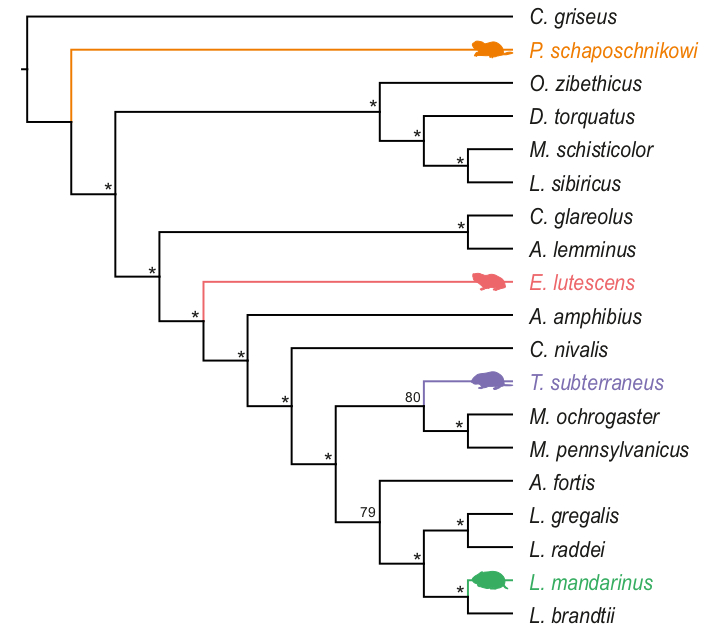
\includegraphics[width=0.5\textwidth]{RNA_tree_colour}
	\end{center}
	\caption{Филогенетическое дерево, построенное при использовании 112 ядерных белок-кодирующих генов. Подземные грызуны отмечены цветом.}\label{tree_RNA}
\end{figure}

\subsection{Анализ частоты несинонимичных замен}

Сравнение частот несинонимичных замен между подземными и наземными видами не показало достоверных различий (рис. \ref{sub_RNA}). Также нами не было обнаружено отдельных генов  или позиций, в которых частоты будут достоверно различаться. 

\begin{figure}[h!]
	\begin{center}
		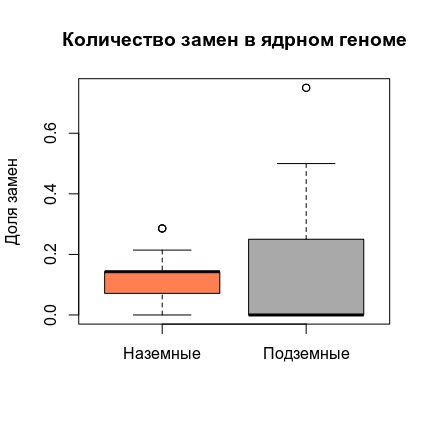
\includegraphics[width=0.5\textwidth]{sub_rna}
	\end{center}
	\caption{Оценка частот несинонимичных замен у подземных и наземных грызунов.}\label{sub_RNA}
\end{figure}

\subsection{Оценка параллельных аминокислотных замен}

При изучении полученных нами ядерных генов мы повторили подход поиска параллельных аминокислотных замен. Нами были обнаружены замены в нескольких генах, где у подземных грызунов она замещалась другой идентичной для всех (<<параллельные>>, таблица \ref{rna_substitution_all}) или замена происходит в той же позиции, но различными аминокислотами (<<дивергентные>>, таблица \ref{rna_substitution_diff}). Последующая статистическая проверкапоказала достоверность замен в генах \textit{Rad23b} и \textit{Pycr2}. 

\begin{table}[h!]
	\caption{Параллельные замены у подземных грызунов, обнаруженные в ядерных генах. Символ «--» означает ту же аминокислоту, что и у наземных видов. \textbf{Жирным} выделены достоверные замены. }\label{rna_substitution_all} \vspace{5mm}
	
	\begin{center}
	\begin{tabular}{|l|c|c|c|c|c|c|c|c|c|c}
		\hline
		\multicolumn{1}{|r|}{Ген} & \textit{Rad23b} & \textit{Hikeshi} & \textit{Mrps14} & \textit{Pycr2} & \textit{GTPBP2} & \textit{Snapc2} \\ \hline
		Вид   / позиция & 121 & 189 & 5 & 314 & 30 & 204  \\ \hline
		Наземные виды &  Thr & Ala & Val & Ala & Val & Glu  \\ \hline
		\textit{P. schaposchnikowi}  & -- & Thr & -- & \textbf{Thr}  & Met & Gly  \\ \hline
		\textit{E. lutestence}  & \textbf{Ala} & -- & Met & \textbf{Thr} & Met & Gly  \\ \hline
		\textit{L. mandarinus}  & -- & -- & -- & --  & -- & --  \\ \hline
		\textit{T. subterraneus} & \textbf{Ala} & Thr  & Met & -- & -- & -- \\ \hline
	\end{tabular}
\end{center}
\end{table}


\begin{table}[h!]
	\caption{Дивергентные замены у подземных грызунов, обнаруженные в ядерных генах. Символ «--» означает ту же аминокислоту, что и у наземных видов.}\label{rna_substitution_diff} \vspace{5mm}
	
	\begin{center}
	\begin{tabular}{|l|c|c|c|c|c|c|c|c|c|c}
		\hline
		\multicolumn{1}{|r|}{Ген} & \textit{Erp29} & \textit{Zadh2} & \textit{Ccdc86} & \textit{Ttll12} \\ \hline
		Вид   / позиция & 255 & 162 & 125 &  91 \\ \hline
		Наземные виды & Ala & Ala & His & Gln \\ \hline
		\textit{P. schaposchnikowi} & Val & Val & -- & -- \\ \hline
		\textit{E. lutestence} & Thr & Thr & Pro & Arg \\ \hline
		\textit{L. mandarinus} & -- & -- & Arg  & -- \\ \hline
		\textit{T. subterraneus} & -- & -- & -- & Lys \\ \hline
	\end{tabular}
\end{center}
\end{table}

\subsection{Оценка уровня отбора} 


Мы провели поиск следов отбора в найденных нами ортологичных генах независимо для каждой линии подземных грызунов (рис. \ref{RNA_trees_sep}). Однако генов с достоверными отличиями обнаружено не было. 

\begin{figure}[h!]
	\begin{center}
		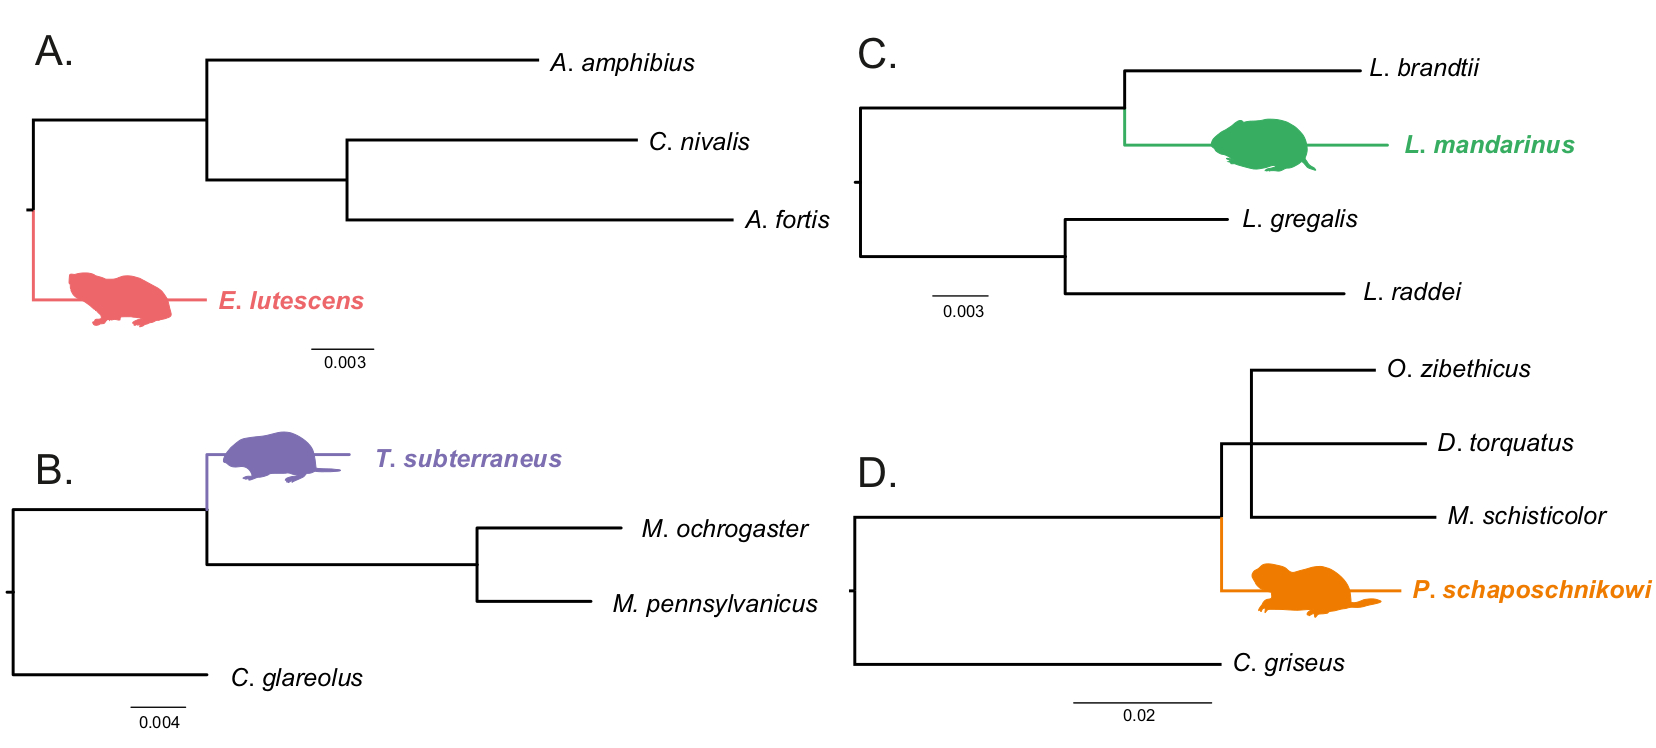
\includegraphics[width=\textwidth]{separate trees_RNA_color}
	\end{center}
	\caption{Филогенетические деревья, использованные для оценки отбора отдельных ветвей. Подземные виды обозначены цветом. Для каждого подземного вида или группы видов использовались филогенетически близкие наземные таксоны.}\label{RNA_trees_sep}
\end{figure} %Результаты
\chapter{Обсуждение} \label{discussion}

\section{Изменения на молекулярном уровне у полевочьих, перешедших к подземному образу жизни}

В нашей работе получены данные по изменению уровня отбора в митохондриальных генах подземных грызунов, а также обнаружены характерные для них параллельные замены в ядерных генах. Помимо этого, мы сравнивали базовые характеристики митохондриальных геномов: GC-состав, его смещение, количество и порядок генов. 

\subsection{Изменение нуклеотиного состава митохондриальных геномов}

Оценка GC-состава показывает повышение количества этих нуклеотидов у подземных грызунов. Уровень смещения (GC-skew) у подземных грызунов сильнее, чем у наземных грызунов. Оно может быть связано с изменением количества нуклеотидов GC-пары. Несмотря на то, что разница в обоих случаях недостоверна, это может указывать на адаптивные следы в митохондриальном геноме. 

Смещение в сторону повышенного содержания A/T наблюдается в мтДНК многих видов (\cite{Ballard2004}). Это может быть вызвано факторами, влияющими на скорость повреждения ДНК (\cite{Martin1995}) и относительную доступность каждого нуклеотида в клеточной среде митохондрии (\cite{Xia1996}). AT-богатые геномы могут реплицироваться быстрее, чем GC-богатые и, при прочих равных, обладают избирательным преимуществом в гетероплазматической популяции (\cite{Ballard2000}). Поскольку у подземных грызунов снижен общий метаболический уровень, может также снижаться и скорость репликации митогеномов. Это, в том числе, и может повлечь обогащение GC-нуклеотидами и, помимо этого, обеспечить большую устойчивость перед активными формами кислорода. Зависимость между обогащением GC-нуклеотидов и увеличением значения GC-skew показана в работе (\cite{Saccone2000}), и вполне ожидаемо было обнаружить разницу в этом значении между подземными и наземными видами. 

Генный состав митохондрий среди всех изученных видов остается стабильным и неизменным. Переход к подземному образу жизни не повлек за собой изменение в порядке генов или удвоение каких-то конкретных блоков. 

\subsection{Ослабление уровня отбора}

Исторически, изучение адаптивности митохондриальных генов началось с гена \textit{CYTB}. Начатые с трудов Эндрюс (\cite{Andrews1998}), и в последующем повторенные целым рядом исследователей (\cite{Tomasco2014}; \cite{DaSilva2009}; \cite{DiRocco2006}; \cite{Shao2015}), работы свидетельствовали о наличии признаков положительного отбора при эволюции гена \textit{CYTB}. Дальнейшие исследования показали, что, несмотря на сильные функциональные ограничения, митохондриальная ДНК в целом может подвергаться положительному направленному отбору, например, в случаях, когда требуется энергоемкий образ жизни и/или есть ограничения в доступности кислорода (\cite{Tomasco2011}; \cite{Shen2010}; \cite{Blier2001}).

Нево (\cite{Nevo1999}) связывал изменения в гене \textit{CYTB} с экологическими различиями между хромосомными расами слепышей \textit{Spalax ehrenbergi}. Da Silva с коллегами (\cite{DaSilva2009}) обнаружили достоверную разницу в соотношении \textit{dN}/\textit{dS} ($\omega$) в независимых линиях подземных грызунов по сравнению с их наземными сестринскими видами. Это предполагает связь между эволюцией гена \textit{CYTB} и освоением гипоксической среды. Позднее это наблюдение было подтверждено для всех митохондриальных белок-кодирующих генов \textit{Octodontidae} (\cite{Tomasco2011}).

В нашем исследовании гена \textit{CYTB} мы также обнаружили ослабление отбора у некоторых подземных грызунов. Применяя стандартные подходы, мы показали, что (1) несколько филогенетически далеких подземных видов имеют одинаковые аминокислотные замены в цитохроме b, и эти замены, вероятно, важны для структуры белкового комплекса, (2) в последовательности гена \textit{CYTB} повышено соотношение между несинонимичными и синонимичными заменами ($\omega$) у подземных грызунов по сравнению с наземными и (3) восемь белковых доменов обладают повышенной частотой замен у подземных видов, тоже наблюдается в нескольких нуклеотидных позициях. Эти результаты согласуются с гипотезой о том, что колонизация подземной ниши способствует положительному отбору в генах мтДНК.

Признаки усиления положительного отбора были выявлены как при сравнении четырех видов \textit{Ellobius} с \textit{Arvicola}, \textit{Eothenomys} и \textit{Chionomys}, так и у \textit{L. mandarinus} при сравнении с другими видами \textit{Lasiopodomys} и \textit{Neodon}. Мы обнаружили достоверную разницу в значениях $\omega$, сравнивая \textit{T. subterraneus} с другими видами \textit{Terricola} и \textit{Microtus}, но в этом случае соотношение \textit{dN}/\textit{dS}, наоборот, было меньше для \textit{T. subterraneus}. Данные анализа RELAX согласуются с результатами codeml и показывают, что ген \textit{CYTB} у подземных грызунов подвержен ослаблению уровня отбора.


Результаты, полученные нами при исследовании всех белок-кодирующих митохондриальных генов, также говорят о вовлеченности митохондриального генома в адаптивный процесс. Метод оценки отбора по отдельным ветвям (branch model), который считается более точным и чувствительным, показал повышение уровня отбора в белок-кодирующих генах у подземных грызунов. Однако, мы наблюдаем различие в количестве генов с достоверным отличием у разных видов. Больше всего различий обнаружено у представителей рода \textit{Ellobius}: разница в отборе наблюдается во всех митохондриальных генах, кроме \textit{ND2,3,5,6} и \textit{COX3}. Два гена под отбором обнаружено у \textit{L. mandarinus}: \textit{COX3} и \textit{CYTB} и только один ген у \textit{Prometheomys} -- \textit{COX3}. У оставшихся представителей подземных грызунов не было обнаружено генов с достоверным отличием. Анализ RELAX подтвердил ослабление уровня отбора в митохондриальных генах у разных видов. Так, у представителей рода \textit{Ellobius} ослабление отбора наблюдается в 8 генах, у \textit{Prometheomys} --- в пяти (при сравнении с первой радиацией) и одном при сравнении с хомяками. Для \textit{L. mandarinus} разница обнаружена в трех генах.  

Проводя поиск следов измнения отбора в генах подземных Arvicolinae мы обнаруживаем гены, которые показывают достоверные различия для более чем одного проанализированного подземного вида и гены, обнаруженные в более чем в одном анализе. Так, гены \textit{CYTB} и \textit{COX3} продемонстрировали более высокие значения $\omega$ одновременно у видов \textit{P. schaposchnikowi} и \textit{L. mandarinus} (\textit{COX3}) и \textit{L. mandarinus} и \textit{Ellobius} (\textit{CYTB}) при оценке уровня отбора методом codeml. Гены \textit{COX3}, \textit{COX1}, \textit{ND2} и \textit{ND4} демонстрируют ослабление отбора согласно программе RELAX по крайней мере для двух видов. Гены \textit{COX1} и \textit{COX3} были обнаружены как наиболее изменчивые при сравнении результатов нескольких программ. 

Набор генов с разницей в уровне отбора у подземных и наземных грызунов частично положительно коррелирует со скоростью их эволюции. Скорости изменчивости среди семейств митохондриальных генов распределяются следующим образом: \textit{ATP}> \textit{ND}> \textit{CYTB}> \textit{COX} согласно Лопесу (\cite{Lopez1997}). По нашим результатам, оба гена \textit{ATP} (\textit{ATP6} и \textit{ATP8}) показывают достоверную разницу в уровне отбора для представителей рода \textit{Ellobius} по сравнению с наземными видами. Кроме того, они выявляются в других анализах: RELAX (\textit{ATP6} для рода \textit{Ellobius}) и aBSREL (\textit{ATP8} для \textit{P. schaposchnikowi}). Гены семейства \textit{ND} показывают неоднородность в результатах. Среди всех генов этого семейства для генов \textit{ND2}, \textit{ND4} и \textit{ND5} обнаружены достоверные различия для трех из пяти проанализированных подземных видов. Ген \textit{CYTB} показывает достоверную разницу в уровне $\omega$ между подземными и наземными видами и подтверждает ослабление отбора для видов \textit{Ellobius} и \textit{L. mandarinus}. Эти результаты повторяют полученные при анализе отдельно гена \textit{CYTB} (\cite{Bondareva2021}). Неожиданный результат получен для генов семейства \textit{COX}: не смотря на свой консерватизм, они показывают достоверные изменения в уровне отбора во всех анализах на том же уровне, что и более вариабельные гены \textit{ND}.


Независимые исследования различных подземных грызунов показали адаптации в митохондриальных генах. Да Силва с коллегами (\cite{DaSilva2009}) обнаружили достоверную разницу в значениях $\omega$ в последовательностях \textit{CYTB} независимых линий подземных грызунов (\textit{Ctenomys},\textit{Spalacopus}, семейство \textit{Geomyidae} и семейство \textit{Bathyergidae}) по сравнению с их назмеными близкородственными видами (\cite{Tomasco2014}). Результаты Zhang предполагали, что эволюция гена \textit{CYTB} цокора \textit{Eospalax cansus} также в основном определяется изменением уровня отбора. Более того, распределение несинонимичных мутаций указывало на значительные изменения в последовательности \textit{CYTB} у животных, которые столкнулись с более тяжелой гипоксией из-за большей высоты и более холодного и сухого климата, чем другие митохондриальные линии (\cite{Zhang2013a}. Наконец, Tomasco и Lessa (\cite{Tomasco2011}) обнаружили повышенные значения $\omega$ в гене \textit{COX2} подземных восьмизубов (почти в 30 раз) и туко-туко (в 11 раз) по сравнению с наземными родственными видами. Позже эти авторы (\cite{Tomasco2011}) показали достоверно более высокие значения $\omega$ для тех же видов по сравнению с наземными в 11 из 13 митохондриальных генов. Конвергентные изменения были также обнаружены между изученными подземными видами и другими млекопитающими, адаптированными к гипоксии. Taveres и коллеги выявили достоверное ослабление отбора в большинстве митохондриальных генов подземных африканских землекопов, туко-туко и восьмизубов (\cite{Tavares2018}). Исследования пищухи \textit{Ochotona curzoniae} показали пятнадцать новых аминокислотных замен, в том числе три в субъединицах цитохром с оксидазы. Эти замены потенциально влияют на модуляцию митохондриальных комплексов и эффективность переноса электронов при адаптации к холоду и гипоксии (\cite{Luo2008}).

 
С одной стороны, наши данные согласуются с опубликованным ранее работами и показывают, что митохондриальный геном подземных полевочьих также потенциально вовлечен в процесс адаптации к подземному образу жизни. Но с другой, мы видим различие в уровне отбора между разными видами. Потенциально, это может быть связано с уровнем и способом специализации к подземному образу жизни.

 
К сожалению, обнаруженная на митохондриальных геномах тенденция к ослаблению отбора не подтвердилась на ядерных данных и нам не удалось найти генов, уровень отбора в которых достоверно бы различался у подземных и наземных грызунов. Это может быть связано как с более медленными темпами эволюции ядерных генов (\cite{Lin2004}) по сравнению с митохондриальными, так и с недостаточным количествов генов, взятых в анализ. Например, в работе Kalina Davies (\cite{Davies2018}) по исследованию адаптаций подземных млекопитающих только в 10\% от всех проанализированных генов (которых было около 8 тыс) обнаружена достоверная разница в отборе между подземными и наземными видами.    


\subsection{Возникновение параллельных замен}

Поиск параллельных замен показал себя как действенный способ обнаружить гены, которые могут быть вовлечены в адаптационные процессы и при этом не меняют уровень или направление отбора (\cite{Davies2018}, \cite{Zhou2015}, \cite{Sackman2017}). 

При анализе отдельно гена \textit{CYTB} нами было обнаружено три замены, характерные для подземных грызунов: Ser57Pro, Asp214Asn, и Ile338Val. Замещение в сайте 57 также обнаружено у африканских слепышей (семейство Bathyergidae) и в 214 - у африканских слепышей и туко-туко (род Ctenomys). Аналогичное замены в сайте 214 были обнаружены у высокогорных подземных цокоров \textit{Eospalax fontanierii} (\cite{Cooper1993}). Cреди подземных полевок замена Asp214Asn была обнаружена у \textit{Prometheomys schaposchnikowi}, \textit{Ellobius fuscocapillus} и \textit{Ellobius lutescens}, а такая же у представителей большинства специализированных семейств подземных грызунов.

Выполняя изначальный поиск на одиночных митохондриальных геномах (т.е. имея только один вариант митохондриального генома для одного вида), у нас была возможность проверить найденные замены на популяционном уровне в гене \textit{CYTB}. Использование его как основного филогенетического маркера позволило включить в полномасштабный популяционный анализ более 6 тыс сиквенсов. Из трех позиций, обнаруженных при анализе, две подтвердились: Thr56Ser и Ile338Val. В них мы видим достоверное смещение использования аминокислот у подземных грызунов: процесс ослабления отбора и большую вариативность в аминокислотном составе. К сожалению, возможности проверить найденные замены на популяционном уровне в других митохондриальных генах не представляется возможным из-за отсутствия достаточного на данный момент количества данных. 


При анализе собранных митохондриальных геномов нами было обнаружено шесть позиций с характерными для подземных грызунов заменами: \textit{COX1} Met73Ile, \textit{COX3} Ile121Val, \textit{ND5} Phe446Leu, \textit{CYTB} Thr56Ser, \textit{CYTB} Ile338Val, \textit{CYTB} Ala357Thr. К сожалению, все выявленные замены оказались недостоверными при статистической проверке. 

 
Повторив поиск на ядерных геномах, нам удалось найти несколько генов с параллельным аминокислотными заменами, которые есть только у подземных грызунов: \textit{Erp29}, \textit{Rad23b}, \textit{Hikeshi}, \textit{Zadh2}, \textit{Mrps14}, \textit{Pycr2}, \textit{Ccdc86}, \textit{GTPBP2}, \textit{Snapc2} и \textit{Ttll12}. Последующая проверка показала достоверность замен в генах \textit{Rad23b} и \textit{Pycr2}.
            
Согласно литературе, обнаруженное нами небольшое число генов (11\% от общего проанализированного числа) с уникальными заменами  является нормальным и ожидаемым. Так, в работе Kalina Davies (\cite{Davies2018}) было обнаружено всего 35 генов с паралельными заменами у всех проанализированных видов (от общего количества проанализированных генов это меньше 1\%), а большее количество составляли гены с уникальными заменами (в нашей работе мы не рассматривали эти варианты) и парными среди разных родов. 

Найденные нами ядерные гены не выявлялись ранее при изучении подземных грызунов, в отличие от митохондриальных. Однако, биохимические пути и процессы, в которые они вовлечены, можно связать с процессами адаптации подземных грызунов. Активная работа митохондрий, которая может быть усилена в условиях сниженной концентрации кислорода, потенциально вызывает образование активных форм кислорода, являющихся опасным для клетки разрушающим фактором (\cite{Turrens2003}). Гены \textit{Rad23b} и \textit{Pycr2} (pyrroline-5-carboxylate reductase 2) связаны с процессами репарации ДНК (\cite{Pohjoismaki2012}) и реакцией на окислительный стресс (\cite{Kuo2015}), соответственно. Гомолог гена \textit{Rad23} был обнаружен при изучении адаптаций к засухе у растений, поскольку его уровень отбора сильно изменялся в сторону положительного (\cite{Zhang2013b}). Изменение его экспрессии также выявлен при анализе устойчивости к холоду \textit{Thinopyrum intermedium} (\cite{Jaikumar2020}).   
       

\section{Конвергентные молекулярные адаптации грызунов к подземному образу жизни}

Мы наблюдаем у подземных полевочьих тенденцию проявления молекулярных адаптаций, описанную ранее в литературе, не смотря на ограниченную выборку полученных и проанализированных генов. В первую очередь, у них независимо ослабляется отбор на митохондриальных генах и увеличивается частота несинонимичных замен в целом. Как в митохондриальных, так и в ядерных генах происходят параллельные аминокислотные замены в физиологически важных генах. 


По некоторым предположениям, повышение уровня отбора в митохондриальных генах могло быть следствием низкой эффективной численности популяции подземных грызунов (\cite{Lacey2000}). Однако, факты, что мы видим этот тренд 1) не во всех генах у одного рода и 2) не у всех видов подземных грызунов, скорее противоречит выдвинутой гипотезе. 

Анализ митохондриальных геномов и транскриптомов показал общие характеристики для подземных грызунов: увеличение уровня отбора и повышение частоты несинонимичных замен в митохондриальных генах, наличие параллельных аминокислотных замен как в митохондриальных, так и в ядерных генах. Однако, если анализировать каждую подземную линию независимо, видна неоднородность проявления этих признаков (рис. \ref{Convergent_arv}). Так, больше всего изменений затронуло род \textit{Ellobius}, а меньше всего -- \textit{Hyperacrius}. Наблюдаемое количество изменений не коррелирует со временем появления вида. Переход к подземному образу жизни у \textit{P.schaposchnikowi} произошел, согласно молекулярным данным, 7 млн лет назад. Но при этом вид не демонстрирует самое большое количество обнаруженных молекулярных изменений. Самое большое количество генов в обоих случаях наблюдается у представителей рода \textit{Ellobius}, хотя их переход к подземному образу жизни был совершен в плиоцене. Несмотря на это, морфологические изменения представителей этого рода наиболее близки к тем, что наблюдаются у <<модельных>> подземных грызунов семейств Bathyergidae и Spalacidae: выступающие резцы, очень маленькие глаза и изолирование ротового отдела губами (\cite{Gromov1977}). 

\begin{figure}[h!]
	\begin{center}
		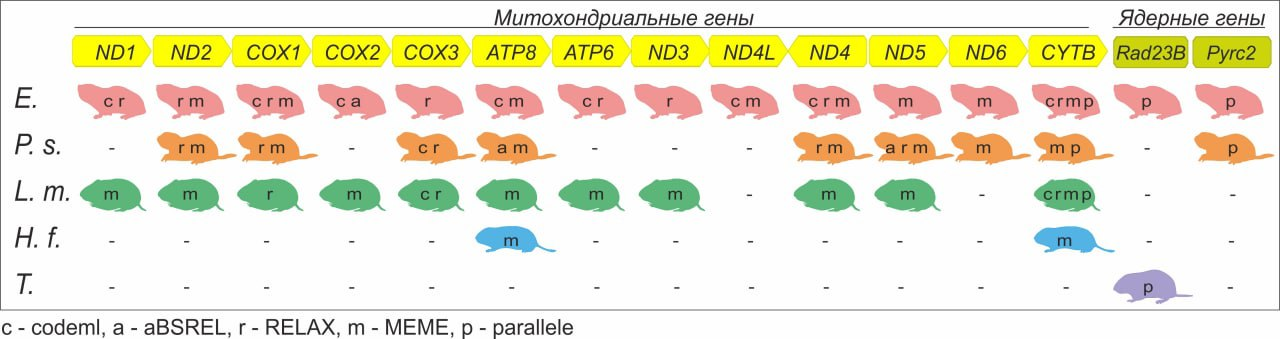
\includegraphics[width=\textwidth]{genes_mt_and_nucl}
	\end{center}
	\caption{Гены с достоверными изменениями уровня отбора для каждого из подземных видов. Буквы внутри каждого силуэта обозначают анализы, в которых был получен достоверный результат. E --- виды рода \textit{Ellobius}, P.s. --- \textit{P. schaposchnikowi}, L.m. --- \textit{L. mandarinus}, H.f. -- \textit{H. fertilis}, T. — виды рода \textit{Terricola}.} \label{Convergent_arv}
\end{figure}

 Самыми стрессовыми факторами, с которыми сталкиваются подземные грызуны, являются гипоксические / гиперкапнические условия и перегрев в закрытой системе нор (\cite{Lacey2000}). Хотя и слепушонки, и \textit{P.schaposchnikowi} являются высокоспециализированными подземными грызунами, они занимают разные среды обитания, и характеристики их нор, а также методы добычи пищи весьма различны. Типичные места обитания \textit{Ellobius} --- засушливые или полузасушливые ландшафты, такие как степи, пустыни и луга. Эти грызуны населяют различные типы почв, в том числе плотные почвы глинистых пустынь, и создают довольно устойчивые системы узких туннелей для кормления под землей (\cite{Ognev1950}; \cite{Gromov1977}; \cite{Shubin1978}). Таким образом, слепушонки должны справляться с проблемами, с которыми сталкиваются другие действительно подземные млекопитающие (\cite{Lacey2000}). Последнее, в свою очередь, может привести к наблюдаемым нами изменениям в белок-кодирующих генах. Напротив, \textit{P.schaposchnikowi} встречается на кавказских субальпийских высокотравных лугах на высоте 1500-2500 м (\cite{Vereshchagin1959}; \cite{Vorontsov1966}; \cite{Krystufek2005}). Его норы вырыты в рыхлой влажной почве, заполненной камнями, что должно увеличить диффузию газа. Важно отметить, что поверхностные кормовые туннели этих полевок необычны тем, что они кажутся слишком большими и почти вдвое шире, чем можно было бы ожидать от грызунов такого размера (\cite{Vorontsov1966}; личные наблюдения А.В. Сморкачевой). Это дополнительное пространство может предотвратить перегрев, гипоксию и гиперкапнию. Кроме того, \textit{P.schaposchnikowi} строго травояден, по крайней мере, летом. Во время кормления полевка высовывается из норы, подбирает растения и затаскивает их в нору для безопасного кормления (\cite{Gambaryan1957}; \cite{Zimina1977}; личные наблюдения А.В. Сморкачевой). Таким образом, даже будучи ограниченными в поисках пищи вблизи отверстий для нор, они на самом деле проводят много времени вне туннелей. Благодаря холодному климату, архитектуре нор и особенностям кормления, \textit{P.schaposchnikowi} может избежать некоторых физиологических проблем, с которыми приходится сталкиваться большинству подземных видов.

У \textit{L. mandarinus}, несмотря на обнаруженные ранее изменения в циркадных ритмах и адатпации к гипоксии (\cite{Sun2018}; \cite{Dong2020}), мы наблюдаем не такие сильные изменения в изученных нами генах: всего три гена с изменением уровня отбора --- \textit{COX1}, \textit{COX3} и \textit{CYTB}. Тем не менее, мы обнаружили существенные различия у \textit{Lasiopodomys mandarinus} и \textit{Terricola}, несмотря на схожий эволюционный возраст этих таксонов. Это различие также может отражать неравные уровни энергетического и гипоксического стресса, возникающие из-за специфических характеристик стратегии поиска пищи и архитектуры норы. \textit{Lasiopodomys mandarinus} питаются либо под землей, либо зелеными частями растений в непосредственной близости от входа в нору. Кормовые ходы этого вида расположены на глубине 10-30 см (\cite{Smorkatcheva1990}; \cite{Hong2019}), а прямые измерения концентрации газов, температуры и влажности подтвердили, что животные в норе должны столкнуться с гипоксией и гиперкапнией. \textit{Terricola} населяют различные растительные сообщества от широколиственных лесов (\textit{T. subterraneus}) до альпийских лугов (\textit{T. daghestanicus}) (\cite{Aulagnier2018}). Подобно \textit{Ellobius}, \textit{Prometheomys} и \textit{L. mandarinus}, они используют сложную сеть подземных тоннелей и демонстрируют некоторые внешние черты, связанные с подземным образом жизни (\cite{Aulagnier2018}; \cite{Mironov2020}). Однако телосложение и повадки \textit{T. subterraneus} (Абрамсон и Сморкачева, неопубликовано), а также характеристики его туннельной системы отличают эту полевку от специализированных подземных грызунов. Пищевые пути этого вида располагаются в самом поверхностном слое почвы (в пределах 5--10 см) или даже непосредственно под опадом листьев (\cite{Mironov2020}). Туннели обеспечивают защиту полевок от неблагоприятных погодных условий и хищников, что объясняет тенденцию видов \textit{Terricola} к снижению скорости базовых метаболических процессов (\cite{Caroli2000}; \cite{Jemiolo1983}; \cite{Schropfer1977}), но их глубина, вероятно, слишком мала, чтобы существенно предотвратить диффузию газа, приводящую к гипоксическим / гиперкапническим условиям внутри. К сожалению, об экологии \textit{T. daghestanicus}, населяющего кавказские альпийские степи и луга, почти ничего не известно. Тот факт, что полевки этого вида, как сообщается, находят убежище среди скал (\cite{Krystufek2005}), предполагает, что они не так строго подземные. Наши результаты подтверждают этот факт, поэтому мы не обнаружили никаких изменений уровня отбора в митохондриальных генах этого вида. 

 Подземные полевочьи повторяют адаптационный путь других подземных грызунов, показывая схожие признаки (таблица \ref{convergent_all}). Так, во время многочисленных исследований представителей семейств Bathyergidae и  Spalacidae были обнаружены параллельные замены в абсолютно разных генах. Также во многих генах видно ослабление отбора и увеличение его уровня по сравнению с наземными. Этот эволюционный тренд подтверждается не только на подземных грызунах, но и на других подземных млекопитающих --  Talpidae и Chrysochloridae. Обнаруженные адаптации митохондриального генома (увеличение уровня отбора, наличие параллельных замен) совпадают с исследованиями на Octodontidae и Ctenomyidae. Таким образом, полученные нами результаты согласуются с гипотезой о том, что переход к подземному образу жизни стимулирует ослабление уровня отбора. Причем выраженность скорее связана с уровнем специализации вида, нежели с возрастом его появления.


%\begin{landscape}
%	
%	\begin{table}[]
%		\caption{Конвергентная эволюция у подземных Arvicolinae. MT -- митохондриальный геном, RNA -- транскриптом. NA -- анализ не проводился, нет -- признаки отсутствуют.}\label{convergent} \vspace{5mm}
%		
%		\begin{tabular}{|c|p{5cm}|p{3.5cm}|p{3.5cm}|p{3.5cm}|p{3.5cm}|p{3.5cm}|}
%			\hline
%			&  & \multicolumn{1}{c|}{\textit{Ellobius sp.}} & \multicolumn{1}{c|}{\textit{P. schaposchnikowi}} & \multicolumn{1}{c|}{\textit{Terricola}} & \multicolumn{1}{c|}{\textit{L. mandarinus}} & \multicolumn{1}{c|}{\textit{H. fertilis}} \\ \hline
%			\multirow{2}{*}{MT} & Гены под отбором & \textit{ATP}6,8,   \textit{COX}1-2, \textit{ND}1, 4, 4L & \textit{COX3} & нет & \textit{COX3}, \textit{CYTB} & нет \\ \cline{2-7}
%			& Параллельные   замены & \textit{CYTB}– 56, 338 & \textit{CYTB} – 56 & нет & \textit{CYTB} – 56, 338 & нет \\ \hline
%			\multirow{2}{*}{RNA} & Гены под отбором & нет & нет & нет & нет & NA \\ \cline{2-7}
%			& Параллельные   замены &  \textit{Rad23b}, \textit{Pycr2} & \textit{Pycr2}& \textit{Rad23b} & нет & NA \\ \hline
%		\end{tabular}
%	\end{table}
%	
%\end{landscape}

\begin{landscape}

\begin{table}[]
	\caption{Конвергентная эволюция у подземных млекопитающих. MT -- митохондриальный геном.}\label{convergent_all} \vspace{5mm}
	
	\begin{tabular}{|p{3cm}|p{3cm}|p{2.8cm}|p{2.7cm}|p{3.4cm}|p{2.7cm}|p{3.3cm}|p{2.8cm}|}
		\hline
		\multicolumn{1}{|c|}{} & \textbf{Arvicolinae (\textit{Ellobius, Prometheomys, Lasiopodomys})} & \textbf{Octodontidae (\textit{Spalacopus})} & \textbf{Ctenomyidae (\textit{Ctenomys})} & \textbf{Bathyergidae (\textit{Heterocephalus, Fukomys, Cryptomys})} & \textbf{Talpidae (\textit{Condylura})} & \textbf{Chrysochloridae (\textit{Amblysomus, Chrysoschoris})} & \textbf{Spalacidae (\textit{Spalax})} \\ \hline
		Ослабление очищающего отбора (МТ) & увеличение уровня & увеличение уровня & увеличение уровня & нет данных & нет данных & нет данных & нет данных \\ \hline
		Ослабление очищающего отбора (ядерные гены) & как у наземных & нет данных & нет данных & увеличение уровня & увеличение уровня & увеличение уровня & увеличение уровня \\ \hline
		Параллельные замены & \textit{Rad23b, Pycr2, CYTB} & нет данных & нет данных & \textit{ARG1, A2M, ABCC3...} & \textit{A2M, ABCC3, C3...} & \textit{A2M, ABCC3, C3...} & \textit{ARG1, A2M...} \\ \hline
	\end{tabular}
\end{table}

\end{landscape} %Обсуждение

\chapter{Заключение} 

Представители полевочьих, ведущие подземный образ жизни, демонстрируют изменение силы и направления отбора в митохондриальных генах, а также имеют характерные для них параллельные замены в ядерных генах. При анализе только одного митохондриального гена \textit{CYTB} мы показали, что в последовательности повышено соотношение между несинонимичными и синонимичными заменами ($\omega$) у  подземных грызунов по сравнению с наземными и восемь белковых доменов обладают повышенной частотой замен у подземных видов. Результаты, полученные нами при исследовании белок-кодирующих митохондриальных генов, говорят о вовлеченности всего митохондриального генома в адаптивный процесс. Анализы показали повышение уровня отбора в митогеномах у подземных грызунов. Однако, мы наблюдаем различие в количестве генов с достоверным отличием выявленных признаков отбора у разных видов: больше всего таких генов обнаружено у представителей рода \textit{Ellobius}. Обнаруженная у митохондриальных геномов тенденция к ослаблению отбора не подтвердилась на ядерных данных, и нам не удалось найти генов, уровень отбора в которых достоверно бы различался у подземных и наземных грызунов. 

При анализе параллельных аминокислотных замен нами было обнаружено три замены в гене \textit{CYTB}: Ser57Pro, Asp214Asn, и Ile338Val. Замена в сайте 57 также обнаружена у землекопов (семейство Bathyergidae), а в 214 -- у землекопов и туко-туко (род \textit{Ctenomys}). Cреди подземных полевок замена Asp214Asn была обнаружена у \textit{Prometheomys schaposchnikowi}, \textit{Ellobius fuscocapillus} и \textit{Ellobius lutescens}, а такая же у представителей большинства специализированных семейств подземных грызунов (Spalacidae, Bathyergidae). Повторив поиск на ядерных геномах, нам удалось найти два гена с параллельным аминокислотными заменами: \textit{Rad23b} и \textit{Pycr2}. Найденные нами ядерные гены не выявлялись ранее при изучении подземных грызунов. Однако, биохимические пути и процессы, в которые они вовлечены, можно связать с процессами адаптации подземных грызунов. Гены \textit{Rad23b} и \textit{Pycr2} (pyrroline-5-carboxylate reductase 2) связаны с процессами репарации ДНК (\cite{Pohjoismaki2012}) и реакцией на окислительный стресс (\cite{Kuo2015}), соответственно. Гомолог гена \textit{Rad23} был обнаружен при изучении адаптаций к засухе у растений, поскольку его уровень отбора сильно изменялся в сторону положительного (\cite{Zhang2013b}). Изменение его экспрессии также выявлен при анализе устойчивости к холоду \textit{Thinopyrum intermedium} (\cite{Jaikumar2020}). 

Анализ митохондриальных геномов и транскриптомов показал общие характеристики для подземных грызунов: усиление отбора и повышение частоты несинонимичных замен в митохондриальных генах, наличие параллельных аминокислотных замен как в митохондриальных, так и в ядерных генах. Однако, если анализировать каждую подземную линию независимо, видна неоднородность проявления этих признаков. Так, больше всего изменений затронуло род \textit{Ellobius}, а меньше всего -- \textit{Hyperacrius}. Наблюдаемое количество изменений не коррелирует со временем появления таксона. Прометеева полевка (\textit{P.schaposchnikowi}) --- древнейший представитель подсемейства, согласно молекулярным данным ее возраст оценивается в 7 млн лет. Но при этом вид не демонстрирует самое большое количество молекулярных следов адаптации к подземным условиям. Самое большое количество генов с признаками адаптивных изменений как в митохондриальном, так и в ядерном геномах наблюдается у представителей рода \textit{Ellobius}, хотя их переход к подземному образу жизни произошел не ранее плиоцена. Несмотря на это, морфологические изменения представителей этого рода наиболее близки к тем, что наблюдаются у <<модельных>> подземных грызунов семейств Bathyergidae и Spalacidae: выступающие резцы, очень маленькие глаза и изолирование ротового отдела губами (\cite{Gromov1977}). 

В целом, подземные полевочьи повторяют адаптационный путь других подземных грызунов, показывая схожие тенденции. Так, во время многочисленных исследований представителей семейств Bathyergidae и Spalacidae были обнаружены параллельные замены в абсолютно разных генах. Также во многих генах видно ослабление отбора и увеличение количества признаков его проявления по сравнению с наземными. Этот эволюционный тренд подтверждается не только на подземных грызунах, но и на других подземных млекопитающих – Talpidae и Chrysochloridae. Обнаруженные адаптивные изменения в митохондриальном геноме полевочьих (изменения уровня отбора, наличие параллельных замен) совпадают с тенденциями, выявленными ранее у Octodontidae и Ctenomyidae. Таким образом, полученные нами результаты согласуются с гипотезой о том, что переход к подземному образу жизни стимулирует ослабление отбора. При этом количество адаптивных сигналов в геноме и их  выраженность положительно коррелирует  с уровнем специализации вида, а не с временем его возникновения.



\chapter{Выводы} 

\begin{enumerate}
	
\item В гене \textit{CYTB} обнаружены параллельные аминокислотные замены, характерные для подземных грызунов и показано увеличение частоты несинонимичных замен.

\item В большинстве генов митохондриального генома наблюдается процесс ослабления отбора у подземных грызунов. 
 
\item При анализе белок-кодирующих генов были выявлены параллельные замены у подземных грызунов, которые вовлечены в разные биохимические процессы. 

\item Количество генов, в которых произошли изменения уровня отбора или возникли параллельные замены, отличаются для разных видов подземных грызунов и связано скорее с уровнем специализации, а не с эволюционным возрастом вида. 

\item Для подземных представителей эволюционно молодого подсемейства полевочьих характерны те же направления молекулярной адаптивной изменчивости, что и для относительно древних специализированных семейств подземных грызунов.
 

\end{enumerate}


\chapter{Публикации автора по теме диссертации}

Основные положения диссертации изложены в семи опубликованных печатных работах в журналах, индексируемых Web of Science и Scopus.

\begin{itemize} 
	\item[\textbullet] \textbf{Bondareva O. V.}, Abramson N. I. The complete mitochondrial genome of the common pine vole \textit{Terricola subterraneus} (Arvicolinae, Rodentia) //Mitochondrial DNA Part B. – 2019. – Т. 4. – №. 2. – С. 3925-3926;
	\item[\textbullet] Abramson N. I. et al. Phylogenetic relationships and taxonomic position of genus \textit{Hyperacrius} (Rodentia: Arvicolinae) from Kashmir based on evidences from analysis of mitochondrial genome and study of skull morphology //PeerJ. – 2020. – Т. 8. – С. e10364;
	\item[\textbullet]\textbf{ Bondareva O. V.} et al. The complete mitochondrial genomes of three \textit{Ellobius} mole vole species (Rodentia: Arvicolinae) //Mitochondrial DNA Part B. – 2020. – Т. 5. – №. 3. – С. 2485-2487. 
	\item[\textbullet] \textbf{Bondareva O. V.} et al. Searching for signatures of positive selection in cytochrome b gene associated with subterranean lifestyle in fast-evolving arvicolines (Arvicolinae, Cricetidae, Rodentia) //BMC Ecology and Evolution. – 2021. – Т. 21. – №. 1. – С. 1-12.
	\item[\textbullet] \textbf{O. Bondareva}, S. Bodrov, E. Genelt-Yanovskiy, T. Petrova, N. Abramson. Signatures of selection and adaptation to subterranean lifestyle across the transcriptomes of Arvicolinae (Rodentia, Cricetidae)// FEBS Open Bio. - 2021. - 11:P-01.3-17. doi:10.1002/2211-5463.13205
	\item[\textbullet] Abramson N. I. et al. Mitochondrial genome phylogeny of voles and lemmings (Rodentia: Arvicolinae): evolutionary and taxonomic implications //Plos One. – 2021. - 16(11): e0248198.
	\item[\textbullet]  \textbf{Bondareva O.}, Genelt-Yanovskiy, E., Petrova, T., Bodrov, S., Smorkatcheva, A., \& Abramson, N.  Signatures of Adaptation in Mitochondrial Genomes of Palearctic Subterranean Voles (Arvicolinae, Rodentia) //MDPI Genes. – 2021. – V. 12. – №. 12. – P. 1945.
\end{itemize}


%Материалы диссертации были представлены на следующих конференциях, конгрессах и мероприятиях:
%\begin{itemize} 
%	\item[\textbullet] Международные конференции по вычислительной биологии MCCMB (Москва, 2017, 2019);
%	\item[\textbullet] XI Международная конференция по биоинформатике и системной биологии BGRS (Новосибирск, 2018); 
%	\item[\textbullet] 16 Международная конференция Rodens et Spatium (Потсдам, Германия, 2018); 
%	\item[\textbullet] VII Международный конгресс общества генетиков и селекционеров ВОГиС (Санкт-Петербург, 2019);
%	\item[\textbullet] Семинары лабораторий териологии и эволюционной геномики и палеогеномики ЗИН РАН (2017-2021);
%	\item[\textbullet] Отчетная сессия ЗИН РАН (Санкт-Петербург, 2020);
%	\item[\textbullet] Семинары лаборатории эволюционной геномики факультета биоинформатики и биоинженерии МГУ (Москва, 2018, 2021);
%	\item[\textbullet] 45th Federation of the European Biochemical Societies (FEBS) Congress (дистанционно, 2021);
%	\item[\textbullet] XI Съезд Териологического общества при РАН (Москва, 2022);
%	\item[\textbullet] Биоинформатический семинар Университета ИТМО (Санкт-Петербург, 2022).
%\end{itemize}       % Выводы
\clearpage                                  % В том числе гарантирует, что список литературы в оглавлении будет с правильным номером страницы
\phantomsection
\addcontentsline{toc}{chapter}{\bibname}	% Добавляем список литературы в оглавление
%%\hypersetup{ urlcolor=black }               % Ссылки делаем чёрными
%%\providecommand*{\BibDash}{}                % В стилях ugost2008 отключаем использование тире как разделителя 
%%\renewcommand*{\bibfont}{\small}
%
\urlstyle{rm}                               % ссылки URL обычным шрифтом
\printbibliography
%%	\insertbibliofull                          % Подключаем Bib-базы
\urlstyle{tt}                               % возвращаем установки шрифта ссылок URL
%%\hypersetup{ urlcolor={urlcolor} }          % Восстанавливаем цвет ссылок


%\chapter*{Список использованной литературы}

%\bibliography{othercites.bib}
 % Список литературы


\appendix
%% Правка оформления ссылок на приложения:
%http://tex.stackexchange.com/questions/56839/chaptername-is-used-even-for-appendix-chapters-in-toc
%http://tex.stackexchange.com/questions/59349/table-of-contents-with-chapter-and-appendix
%% требует двойной компиляции
\addtocontents{toc}{\def\protect\cftchappresnum{\appendixname{} }%
\setlength{\cftchapnumwidth}{\widthof{\cftchapfont\appendixname~Ш\cftchapaftersnum}}%
}
%% Оформление заголовков приложений ближе к ГОСТ:
\sectionformat{\chapter}[display]{% Параметры заголовков разделов в тексте
    label=\chaptertitlename\ \thechapter,% (ГОСТ Р 2.105, 4.3.6)
    labelsep=20pt,
}
\renewcommand\thechapter{\Asbuk{chapter}} % Чтобы приложения русскими буквами нумеровались
   % Предварительные настройки для правильного подключения Приложений
%\chapter{Приложения}

\begin{landscape}


\chapter{Виды, используемые в работе}
%\label{Matheril_Table_PR}

\begin{center}

\begin{longtable}{|p{3.5cm}|p{4.5cm}|p{4.0cm}|p{6.5cm}|p{4.5cm}|}
	\caption{Виды, использованные в работе. Каждому анализу соответствуют отдельные столбцы. \textbf{Жирным} выделены сиквенсы, полученные в группе молекулярной систематики ЗИН РАН. SRA обозначает, что сырые риды были взяты из базы данных SRA, но сборка осуществлялась самостоятельно в группе молекулярной систематики ЗИН РАН; наши данные -- сиквенсы получены в группе молекулярной систематики, но не выложены в открытые базы данных; GenBank assambly -- в анализ взят уже собранный транскриптом из базы данных Genome.} \label{Matheril_Table} \vspace{5mm} \\ 

	\hline \multicolumn{1}{|c|}{\textbf{Род}} & \multicolumn{1}{c|}{\textbf{Вид}} & \multicolumn{1}{c|}{\textit{\textbf{cytB}}} & \multicolumn{1}{c|}{\textbf{Митохондриальные геномы}}  & \multicolumn{1}{c|}{\textbf{Транскриптомы}} \\ \hline 
\endfirsthead

\multicolumn{5}{c}%
{{\tablename\ \thetable{} --- продолжение}} \\

	\hline \multicolumn{1}{|c|}{\textbf{Род}} & \multicolumn{1}{c|}{\textbf{Вид}} & \multicolumn{1}{c|}{\textit{\textbf{cytB}}} & \multicolumn{1}{c|}{\textbf{Митохондриальные геномы}}  & \multicolumn{1}{c|}{\textbf{Транскриптомы}} \\ \hline 
\endhead

\hline \multicolumn{5}{|r|}{{Продолжение на следующей странице}} \\ \hline
\endfoot

\hline \hline
\endlastfoot


\multirow{4}{*}{Alexandromys} & \textit{A. fortis} & AF163894 & NC\_015241 & SRA\\ \cline{2-5}
& \textit{A. kikuchii} & -- & NC\_003041 & --\\ \cline{2-5}
& \textit{A. maximowiczii} & KJ857288 & -- & --\\ \cline{2-5}
& \textit{A. oeconomus} & AY219983 & -- & --\\ \hline
\multirow{7}{*}{Alticola} & \textit{A. argentatus} & KJ556627 & -- & --\\ \cline{2-5}
& \textit{A. barakshin} & KJ556637  & -- & --\\ \cline{2-5}
& \textit{A. lemminus} & KJ556621 & \textbf{MT381922} & \textbf{наши данные}\\ \cline{2-5}
& \textit{A. macrotis} & DQ845196 & \textbf{MT381923} & --\\ \cline{2-5}
& \textit{A. olchonensis} & -- & \textbf{MT381924} & --\\ \cline{2-5}
& \textit{A. strelzowi} & -- & \textbf{MT381925} & --\\ \cline{2-5}
& \textit{A. tuvinicus} & -- & \textbf{MT381926} & --\\ \hline
Arvicola & \textit{A. amphibius} & MF099519  & \textbf{MT381921} & SRA\\ \hline
\multirow{3}{*}{Blanfordimys} & \textit{B. afghanus} & EF599109 & -- & --\\ \cline{2-5}
& \textit{B. carruthersii} & EF599113 & -- & --\\ \cline{2-5}
& \textit{B. juldaschi} & -- & \textbf{MT381927} & --\\ \hline
Caryomys & \textit{C. inez} & -- & KU200225 & --\\ \hline
\multirow{2}{*}{Chionomys} & \textit{C. gud} & JN244677 & \textbf{MT381928} & --\\ \cline{2-5}
& \textit{C. nivalis} & JN244707 & \textbf{MT381934} & \textbf{наши данные}\\ \hline
\multirow{3}{*}{Clethrionomys} & \textit{С. centralis} & -- & \textbf{MT381940} & --\\ \cline{2-5}
& \textit{C. glareolus} & MH197069 & NC\_024538 & SRA\\ \cline{2-5}
& \textit{C. rutilus} & AF119274 & -- & --\\ \hline
\multirow{3}{*}{Craseomys} & \textit{C. regulus} & -- & JN629046 & -- \\ \cline{2-5}
& \textit{C. rex} & AB565454 & -- & --\\ \cline{2-5}
& \textit{C. rufocanus} & AY309418 & NC\_029477 & --\\ \hline
\multirow{3}{*}{Dicrostonyx} & \textit{D. groenlandicus} & -- & NC\_034313 & --\\ \cline{2-5}
& \textit{D. hudsonius} & KY753975 & NC\_034307 & --\\ \cline{2-5}
& \textit{D. torquatus} & AF119275 & NC\_034646 & \textbf{наши данные}\\ \hline
\multirow{4}{*}{Ellobius} & \textit{E. fuscocapillus} & \textbf{MN735805} & \textbf{MT483991} & --\\ \cline{2-5}
& \textit{E. lutescens} & \textbf{MN735804} & \textbf{MT483992} & SRA\\ \cline{2-5}
& \textit{E. talpinus} & \textbf{MN735803} & \textbf{MT483993} & --\\ \cline{2-5}
& \textit{E. tancrei} & AF119270 & -- & --\\ \hline
Eolagurus & \textit{E. luteus} & \textbf{MN735806} & \textbf{MT492448} & --\\ \hline
\multirow{3}{*}{Eothenomys} & \textit{E. chinensis} & -- & NC\_013571 & --\\ \cline{2-5}
& \textit{E. melanogaster} & AY426681 & NC\_027418 & --\\ \cline{2-5}
& \textit{E. miletus} & -- & NC\_030330 & --\\ \hline
Lagurus & \textit{L. lagurus} & AF429818 & \textbf{MT492449} & --\\ \hline
\multirow{4}{*}{Lasiopodomys} & \textit{L. brandtii} & GQ352472 & \textbf{MT381936} & SRA\\ \cline{2-5}
& \textit{L. gregalis} & AY513803 & \textbf{MT381937} & \textbf{наши данные}\\ \cline{2-5}
& \textit{L. mandarinus} & FJ986322 & NC\_025283 & SRA\\ \cline{2-5}
& \textit{L. raddei} & \textbf{KF751080} & \textbf{MT381929} & \textbf{наши данные}\\ \hline
\multirow{2}{*}{Lemmus} & \textit{L. sibiricus} & KY754011 & -- & \textbf{наши данные}\\ \cline{2-5}
& \textit{L. trimicronatus} & AF119276 & \textbf{MT381930} & --\\ \hline
\multirow{14}{*}{Microtus} & \textit{M. agrestis}  & FJ619786 & NC\_041250 & --\\ \cline{2-5}
& \textit{M. arvalis} & AM991041 & NC\_038176 & --\\ \cline{2-5}
& \textit{M. cabrerae} & AY513789 & \textbf{MT381938} & --\\ \cline{2-5}
& \textit{M. californicus} & AF163891 & \textbf{MT381939} & --\\ \cline{2-5}
& \textit{M. guentheri} & AY513806 & \textbf{MT381935} & --\\ \cline{2-5}
& \textit{M. levis} & AY513821 & NC\_008064 & --\\ \cline{2-5}
& \textit{M. longicaudus} & -- & \textbf{MT381942} & \\ \cline{2-5}
& \textit{M. miurus} & GU809171 & \textbf{MT381943} & --\\ \cline{2-5}
& \textit{M. ochrogaster} & AF163901 & NC\_027945 & GenBank assambly\\ \cline{2-5}
& \textit{M. pennsylvanicus} & -- & -- & SRA\\ \cline{2-5}
& \textit{M. pinetorum} & KY754042 & -- & --\\ \cline{2-5}
& \textit{M. qazvinensis} & KM390979 & -- & --\\ \cline{2-5}
& \textit{M. richardsoni} & AF163905 & \textbf{MT381944} & --\\ \cline{2-5}
& \textit{M. socialis} & AY513829 & \textbf{MT381932} & --\\ \hline
Myopus & \textit{M. schisticolor} & AF119263 & \textbf{MT381931} & \textbf{наши данные}\\ \hline
\multirow{4}{*}{Neodon} & \textit{N. fuscus} & JF906122 & NC\_040138 & --\\ \cline{2-5}
& \textit{N. irene} & HQ123595 & NC\_016055 & --\\ \cline{2-5}
& \textit{N. leucurus} & KP190223 & -- & --\\ \cline{2-5}
& \textit{N. sikimensis} & HQ123599 & NC\_035503 & --\\ \hline
Neofiber & \textit{N. alleni} & AM910618 & -- & --\\ \hline
Ondatra & \textit{O. zibethicus} & AF119277 & NC\_036035 & \textbf{наши данные}\\ \hline
Phenacomys & \textit{P. intermedius} & AF119260 & \textbf{MT381941} & --\\ \hline
Proedromys & \textit{P. liangshanensis} & -- & NC\_013563 & --\\ \hline
Prometheomys & \textit{P. schaposchnikowi} & MN735802 & \textbf{наши данные} & \textbf{наши данные}\\ \hline
Synaptomys & \textit{S. cooperi} & DQ323957 & \textbf{MT492450} & --\\ \hline
\multirow{4}{*}{Terricola} & \textit{T. daghestanicus} & AY513791 & \textbf{MT381933} & --\\ \cline{2-5}
& \textit{T. majori} & AY513814 & -- & --\\ \cline{2-5}
& \textit{T. thomasi} & LT222312 & -- & --\\ \cline{2-5}
& \textit{T. subterraneus} & AY513832 & \textbf{MN326850} & \textbf{наши данные}\\ \hline
Volemys & \textit{V. millicens} & JF906123 & -- & --\\ \hline
Dinaromys & \textit{D. bogdanovi} & -- & \textbf{MT588182} & --\\ \hline
Hyperacrius & \textit{H. fertilis} & -- & \textbf{MT433094} & --\\ \hline
\multicolumn{5}{|c|}{OUTGROUP} \\ \hline
Akodon & \textit{A. montensis} & -- & NC\_025746 & --\\ \hline
\multirow{4}{*}{Cricetulus} & \textit{C. griseus} & -- & NC\_007936 & GenBank assambly\\ \cline{2-5}
& \textit{C. kamensis} & -- & NC\_024592 & --\\ \cline{2-5}
& \textit{C. longicaudatus} & -- & NC\_025330 & --\\ \cline{2-5}
& \textit{C. migratorius} & AY288508 & NC\_031802 & --\\ \hline
Mesocricetus & \textit{M. auratus} & KY754035 & -- & --\\ \hline
Phodopus & \textit{P. roborovskii} & KT750095 & -- & --\\ \hline
\multirow{2}{*}{Peromyscus} & \textit{P. ochraventer} &  JX910119 & -- & --\\ \cline{2-5}
& \textit{P. megalops} & -- & NC\_035613 & --\\ \hline


\end{longtable}

\end{center}


\chapter{Анализ популяционной изменчивости гена \textit{cytB}}

\begin{longtable}{|l|l|p{10.5cm}|p{10.5cm}|}
	\caption{Сайты с достоверным отличием частоты использования аминокислот у наземных и подземных видов. Аминокислоты приведены в универсальной однобуквенной кодировке. Holm – значение p-value после поправки на множественное тестирование методом Холма.} \label{BigTable} \vspace{5mm} \\
	
	\hline \multicolumn{1}{|c|}{\textbf{Позиция}} & \multicolumn{1}{c|}{\textbf{Holm}} & \multicolumn{1}{p{6.5cm}|}{\textbf{Наземные виды}} & \multicolumn{1}{p{6.5cm}|}{\textbf{Подземные виды}} \\ \hline 
	\endfirsthead
	
	\multicolumn{4}{c}%
	{{\tablename\ \thetable{} --- продолжение}} \\
	
	\hline \multicolumn{1}{|c|}{\textbf{Позиция}} & \multicolumn{1}{c|}{\textbf{Holm}} & \multicolumn{1}{p{6.5cm}|}{\textbf{Наземные виды}} & \multicolumn{1}{p{6.5cm}|}{\textbf{Подземные виды}} \\ \hline 
	\endhead
	
	\hline \multicolumn{4}{|r|}{{Продолжение на следующей странице}} \\ \hline
	\endfoot
	
	\hline \hline
	\endlastfoot
	
	3 & 0,003 & A:0,00388, I:0,67137, L:0,00071, M:0,00141, N:0,00035, S:0,00106, T:0,00035, V:0,32017, Y:0,00071 & F:0,0177, I:0,95575, V:0,02655 \\ \hline 
	4 & 0,003 & A:0,00035, F:0,00105, I:0,97484, L:0,00175, M:0,01363, N:0,00035, T:0,00035, V:0,00769 & I:0,61062, M:0,36283, T:0,02655 \\ \hline 
	10 & 0,003 & L:0,99935, M:0,00065 & L:0,97345, M:0,02655 \\ \hline 
	11 & 0,016 & A:0,00032, F:0,00032, I:0,99132, L:0,00032, M:0,00257, S:0,00064, V:0,00289, Y:0,00161 & I:0,95575, M:0,00885, T:0,00885, V:0,02655 \\ \hline 
	13 & 0,003 & I:0,8445, K:0,00032, L:0,00664, M:0,1476, V:0,00032, W:0,00063 & I:0,62832, L:0,31858, M:0,0531 \\ \hline 
	17 & 0,003 & A:0,14015, I:0,00031, S:0,85741, T:0,00153, V:0,00061 & A:0,00885, S:0,99115 \\ \hline 
	23 & 0,003 & A:0,83373, R:0,00027, S:0,00348, T:0,16252 & A:0,55814, T:0,44186 \\ \hline 
	33 & 0,003 & C:0,00212, F:0,99618, I:0,00021, L:0,00085, S:0,00021, V:0,00042 & F:0,95385, L:0,04615 \\ \hline 
	40 & 0,018 & C:0,99938, F:0,00041, W:0,00021 & C:0,98462, G:0,00769, W:0,00769 \\ \hline 
	42 & 0,003 & A:0,01348, F:0,00099, I:0,85431, L:0,00079, M:0,09197, T:0,00634, V:0,03211 & A:0,04615, F:0,02308, I:0,67692, S:0,01538, T:0,22308, V:0,01538 \\ \hline 
	43 & 0,003 & A:0,00118, D:0,00039, I:0,75666, M:0,00887, T:0,02189, V:0,211 & I:0,36154, M:0,05385, T:0,16923, V:0,41538 \\ \hline 
	46 & 0,01 & I:0,06471, L:0,93472, S:0,00019, T:0,00038 & L:1 \\ \hline 
	50 & 0,005 & F:0,99946, I:0,00018, L:0,00018, S:0,00018 & F:0,97692, I:0,01538, S:0,00769 \\ \hline 
	56 & 0,003 & I:0,00034, S:0,00272, T:0,99694 & P:0,00769, S:0,04615, T:0,94615 \\ \hline 
	57 & 0,003 & A:0,00136, L:0,00034, P:0,00119, S:0,99643, Y:0,00068 & P:0,0458, S:0,9542 \\ \hline 
	60 & 0,003 & A:0,38586, I:0,00034, S:0,51283, T:0,10097 & A:0,63359, S:0,32824, T:0,03817 \\ \hline 
	66 & 0,008 & L:0,00068, V:0,99932 & I:0,01527, V:0,98473 \\ \hline 
	67 & 0,003 & A:0,49248, S:0,00051, T:0,50668, V:0,00034 & A:0,9771, T:0,0229 \\ \hline 
	69 & 0,003 & I:0,99966, L:0,00034 & I:0,9771, M:0,0229 \\ \hline 
	82 & 0,003 & A:0,01129, G:0,00034, L:0,06625, M:0,91571, T:0,00624, V:0,00017 & L:0,30769, M:0,69231 \\ \hline 
	102 & 0,003 & I:0,23305, L:0,00101, M:0,39155, V:0,37439 & I:0,0687, V:0,9313 \\ \hline 
	118 & 0,003 & F:5e-04, I:0,65786, M:0,00151, N:0,00017, V:0,33995 & I:0,9771, V:0,0229 \\ \hline 
	133 & 0,003 & F:0,00033, L:0,99967 & I:0,01527, L:0,9771, R:0,00763 \\ \hline 
	149 & 0,005 & L:1 & L:0,98462, M:0,01538 \\ \hline 
	160 & 0,003 & L:0,99983, V:0,00017 & I:0,02308, L:0,97692 \\ \hline 
	162 & 0,003 & E:0,99745, K:0,00255 & E:0,89231, K:0,10769 \\ \hline 
	171 & 0,003 & D:0,99557, E:0,00085, N:0,00306, Y:0,00051 & D:0,88462, N:0,11538 \\ \hline 
	178 & 0,005 & F:0,99983, V:0,00017 & F:0,98462, L:0,01538 \\ \hline 
	194 & 0,003 & F:0,37632, L:0,6157, M:0,00799 & L:1 \\ \hline 
	203 & 0,003 & A:0,00036, K:0,00054, S:0,00018, T:0,99893 & S:0,02308, T:0,97692 \\ \hline 
	209 & 0,005 & A:0,06304, I:0,00322, M:0,00036, P:0,00018, S:0,10244, T:0,82611, V:0,00466 & S:0,03077, T:0,96923 \\ \hline 
	212 & 0,003 & D:0,00018, N:0,99982 & D:0,01538, K:0,03846, N:0,94615 \\ \hline 
	215 & 0,003 & A:0,86109, S:0,01828, T:0,12063 & A:0,98462, T:0,01538 \\ \hline 
	221 & 0,003 & H:0,99424, P:0,00558, Y:0,00018 & H:0,88462, P:0,11538 \\ \hline 
	226 & 0,003 & I:0,6858, M:0,00108, T:0,00054, V:0,31258 & I:0,33077, M:0,00769, T:0,02308, V:0,63846 \\ \hline 
	232 & 0,003 & A:0,11343, D:0,00018, G:0,00252, I:0,02485, N:0,00018, V:0,85884 & A:0,32308, I:0,03077, V:0,64615 \\ \hline 
	233 & 0,003 & F:0,00144, I:0,00252, L:0,99586, Q:0,00018 & F:0,03077, L:0,96923 \\ \hline 
	234 & 0,003 & F:0,02035, I:0,91682, L:0,05221, M:0,0027, T:0,00018, V:0,00774 & F:0,00769, I:0,66154, L:0,30769, M:0,02308 \\ \hline 
	237 & 0,003 & K:0,00252, L:0,00036, M:0,96307, S:0,0054, T:0,0281, V:0,00054 & A:0,26154, K:0,12308, M:0,57692, T:0,01538, V:0,02308 \\ \hline 
	238 & 0,003 & A:0,4351, D:0,00018, G:0,3982, S:0,01242, T:0,0036, V:0,1505 & A:0,72308, T:0,26923, V:0,00769 \\ \hline 
	239 & 0,003 & F:0,36712, L:0,63036, S:0,00234, V:0,00018 & F:0,65385, L:0,31538, S:0,03077 \\ \hline 
	240 & 0,003 & I:0,00018, K:0,00072, M:0,99856, Q:0,00018, T:0,00036 & K:0,10769, M:0,87692, T:0,01538 \\ \hline 
	241 & 0,003 & I:0,99027, M:0,00018, N:0,00036, T:0,00504, V:0,00414 & I:0,67692, M:0,27692, T:0,03846, V:0,00769 \\ \hline 
	243 & 0,003 & A:0,11107, G:0,00018, N:0,00018, T:0,32005, V:0,56852 & A:0,3, T:0,65385, V:0,04615 \\ \hline 
	248 & 0,003 & D:0,99802, E:0,00018, H:0,00018, K:0,00018, N:0,00144 & D:0,9, N:0,1 \\ \hline 
	249 & 0,003 & A:0,06564, I:0,48007, L:0,00054, M:0,00036, T:0,00343, V:0,44995 & A:0,23256, F:0,00775, I:0,75194, T:0,00775 \\ \hline 
	256 & 0,003 & D:0,00036, F:0,04833, Y:0,9513 & F:0,28319, Y:0,71681 \\ \hline 
	266 & 0,003 & A:0,43584, P:0,56379, T:0,00037 & A:0,00893, M:0,02679, P:0,96429 \\ \hline 
	275 & 0,016 & I:0,00019, L:0,99926, M:0,00019, P:0,00019, S:0,00019 & I:0,01802, L:0,98198 \\ \hline 
	281 & 0,039 & L:0,99907, V:0,00093 & L:0,98198, V:0,01802 \\ \hline 
	288 & 0,027 & G:0,00019, L:0,99907, M:0,00037, V:0,00037 & L:0,98198, V:0,01802 \\ \hline 
	296 & 0,003 & L:0,99963, P:0,00019, V:0,00019 & L:0,97297, M:0,02703 \\ \hline 
	299 & 0,003 & F:0,00167, L:0,79117, M:0,00056, S:0,00111, V:0,20549 & F:0,00901, I:0,00901, L:0,94595, S:0,02703, V:0,00901 \\ \hline 
	300 & 0,003 & I:0,9358, M:0,00037, N:0,00019, T:0,00019, V:0,06346 & I:0,68468, V:0,31532 \\ \hline 
	302 & 0,003 & A:0,99207, N:0,00019, S:0,0058, T:0,00193 & A:0,81081, T:0,18919 \\ \hline 
	303 & 0,003 & A:0,0642, D:0,00039, F:0,23856, I:0,03491, L:0,66001, M:0,00019, R:0,00019, V:0,00155 & F:0,01802, L:0,98198 \\ \hline 
	304 & 0,003 & I:0,00019, L:0,42658, M:0,57148, N:0,00019, Q:0,00019, V:0,00116, Y:0,00019 & I:0,01802, M:0,98198 \\ \hline 
	305 & 0,01 & P:0,99942, T:0,00058 & P:0,98198, R:0,01802 \\ \hline 
	306 & 0,003 & F:0,03052, H:0,04976, I:0,0344, L:0,8206, M:0,00739, S:0,00019, T:0,00019, Y:0,05695 & F:0,90991, I:0,00901, L:0,08108 \\ \hline 
	311 & 0,045 & K:0,99903, N:0,00058, P:0,00019, V:0,00019 & E:0,00901, K:0,98198, N:0,00901 \\ \hline 
	314 & 0,01 & A:0,35146, F:0,00019, G:0,5193, L:0,00019, S:0,00253, T:0,12632 & A:0,55856, G:0,36937, T:0,07207 \\ \hline 
	324 & 0,02 & C:2e-04, I:0,05851, L:0,00078, M:0,91037, Q:2e-04, V:0,02994 & L:0,00901, M:0,95495, V:0,03604 \\ \hline 
	325 & 0,003 & H:2e-04, P:2e-04, Y:0,99961 & F:0,01802, Y:0,98198 \\ \hline 
	327 & 0,045 & I:0,92446, L:0,0012, M:2e-04, T:0,00381, V:0,07033 & I:1 \\ \hline 
	329 & 0,003 & A:0,001, M:6e-04, T:2e-04, V:0,99819 & I:0,01802, T:0,03604, V:0,94595 \\ \hline 
	331 & 0,003 & D:1 & D:0,96364, N:0,03636 \\ \hline 
	334 & 0,003 & A:0,00143, I:0,70123, L:2e-04, T:0,0135, V:0,28364 & I:0,94595, L:0,00901, T:0,02703, V:0,01802 \\ \hline 
	335 & 0,008 & L:1 & F:0,01802, L:0,98198 \\ \hline 
	338 & 0,003 & I:0,99666, M:0,00022, N:0,00022, V:0,00289 & I:0,94595, V:0,05405 \\ \hline 
	349 & 0,003 & A:0,01107, I:0,89657, M:0,0131, T:0,01265, V:0,06662 & I:0,64865, L:0,01802, M:0,32432, V:0,00901 \\ \hline 
	353 & 0,003 & A:0,04928, H:0,00023, I:0,0636, M:0,38653, P:0,00023, S:7e-04, T:0,47407, V:0,02535 & A:0,01802, L:0,00901, T:0,63063, V:0,34234 \\ \hline 
	357 & 0,01 & A:0,98307, G:0,00072, L:0,00119, S:0,00024, T:0,01479 & A:0,93694, G:0,01802, T:0,04505 \\ \hline 
	360 & 0,003 & A:0,77274, E:0,00024, S:0,00048, T:0,22654 & A:0,07207, T:0,92793 \\ \hline 
	365 & 0,003 & F:0,60583, I:0,00025, L:0,39316, S:0,00051, V:0,00025 & F:0,03604, L:0,95495, P:0,00901 \\ \hline 
	366 & 0,003 & I:0,00026, M:0,99974 & M:0,98198, T:0,01802 \\ \hline 
	369 & 0,014 & A:0,91371, G:0,00026, S:0,07742, T:0,00782, V:0,00078 & A:1 \\ \hline 
	371 & 0,003 & I:0,00999, K:0,00053, L:0,00053, M:0,97529, T:0,0071, V:0,00657 & A:0,00901, I:0,00901, L:0,03604, M:0,82883, V:0,11712 \\ \hline 
	375 & 0,003 & D:0,29643, I:0,00136, K:0,00027, N:0,6853, R:0,00027, S:0,01309, Y:0,00327 & D:0,05455, N:0,94545 \\ \hline 
	377 & 0,003 & L:0,78128, M:0,21844, R:0,00028 & L:1 \\ \hline 
	379 & 0,003 & L:0,98892, M:0,01049, R:3e-04, V:3e-04 & L:0,67273, M:0,32727 \\ \hline 
	380 & 0,003 & D:0,97739, E:0,00428, N:0,01803, T:0,00031 & D:0,66364, N:0,33636 \\  \hline
	
	
\end{longtable}



\chapter{Характеристика собранных митохондриальных геномов}


\begin{longtable}{|l|l|l|c|c|c|c|c|c|c|c|}
	\caption{Характеристика собранных митохондриальных геномов. \textbf{Жирным} выделены виды, полученные в группе молекулярной систематики ЗИН РАН.} \label{mt_stats} \vspace{5mm} \\
	
\hline
\multicolumn{1}{|c|}{\multirow{2}{*}{\textbf{Триба}}} & \multicolumn{1}{c|}{\multirow{2}{*}{\textbf{Род}}} & \multicolumn{1}{c|}{\multirow{2}{*}{\textbf{Вид}}} & \multirow{2}{*}{\textbf{Genbank  No}} & \multicolumn{4}{c|}{\textbf{Нуклеотидный состав}} & \multirow{2}{*}{\textbf{GC \%}} & \multirow{2}{*}{\textbf{GC skew}} & \multirow{2}{*}{\textbf{Длина, пн}} \\ \cline{5-8}
\multicolumn{1}{|c|}{} & \multicolumn{1}{c|}{} & \multicolumn{1}{c|}{} &  & \textbf{T} & \textbf{A} & \textbf{C} & \textbf{G} &  &  &  \\ \hline
				
\endfirsthead

\multicolumn{11}{c}%
{{\tablename\ \thetable{} --- продолжение}} \\

\hline
\multicolumn{1}{|c|}{\multirow{2}{*}{\textbf{Триба}}} & \multicolumn{1}{c|}{\multirow{2}{*}{\textbf{Род}}} & \multicolumn{1}{c|}{\multirow{2}{*}{\textbf{Вид}}} & \multirow{2}{*}{\textbf{Genbank  No}} & \multicolumn{4}{c|}{\textbf{Нуклеотидный состав}} & \multirow{2}{*}{\textbf{GC \%}} & \multirow{2}{*}{\textbf{GC skew}} & \multirow{2}{*}{\textbf{Длина, пн}} \\ \cline{5-8}
\multicolumn{1}{|c|}{} & \multicolumn{1}{c|}{} & \multicolumn{1}{c|}{} &  & \textbf{T} & \textbf{A} & \textbf{C} & \textbf{G} &  &  &  \\ \hline

\endhead

\hline \multicolumn{11}{|r|}{{Продолжение на следующей странице}} \\ \hline
\endfoot

\hline \hline
\endlastfoot
				
				
				\multirow{29}{*}{Arvicolini} & \textit{Arvicola} & \textit{\textbf{A. amphibius}} & \textbf{MT381921} & 30 & 31,6 & 25,8 & 12,6 & 38,687 & -0,333 & 16,085 \\ \cline{2-11} 
				& \textit{Agricola} & \textit{A. agrestis} & NC\_041250 & 27,9 & 30,8 & 27,9 & 13,4 & 35,646 & -0,333 & 16,297 \\ \cline{2-11} 
				& \multirow{2}{*}{\textit{Alexandromys}} & \textit{A. fortis} & NC\_015241 & 27,1 & 30,8 & 28,9 & 13,1 & 36,501 & -0,367 & 16,310 \\ \cline{3-11} 
				&  & \textit{A. kikuchii} & NC\_003041 & 27 & 30,7 & 28,9 & 13,4 & 36,659 & -0,348 & 16,312 \\ \cline{2-11} 
				& \textit{Blanfordimys} & \textit{\textbf{B. juldaschi}} & \textbf{MT381927} & 27,5 & 31,1 & 28,3 & 13,1 & 36,065 & -0,333 & 16,378 \\ \cline{2-11} 
				& \multirow{2}{*}{\textit{Chionomys}} & \textit{\textbf{C. gud}} & \textbf{MT381928} & 29,9 & 31,5 & 25,8 & 12,8 & 33,948 & -0,301 & 16,278 \\ \cline{3-11} 
				&  & \textit{\textbf{C. nivalis}} & \textbf{MT381934} & 28 & 31 & 27,7 & 13,3 & 35,673 & -0,318 & 16,296 \\ \cline{2-11} 
				& \textit{Hyperacrius} & \textit{\textbf{H. fertilis}} & \textbf{MT433094} & 29,6 & 29,1 & 26,7 & 14,6 & 27,467 & -0,200 & 12,524 \\ \cline{2-11} 
				& \textit{Iberomys} & \textit{\textbf{I. cabrerae}} & \textbf{MT381938} & 27,4 & 29,6 & 28,5 & 14,4 & 37,143 & -0,318 & 16,327 \\ \cline{2-11} 
				& \multirow{4}{*}{\textit{Lasiopodomys}} & \textit{\textbf{L. brandtii}} & \textbf{MT381936} & 28,5 & 30,2 & 27,3 & 14 & 35,989 & -0,303 & 16,315 \\ \cline{3-11} 
				&  & \textit{\textbf{L. gregalis}} & \textbf{MT381937} & 27,5 & 30,2 & 28,3 & 14 & 36,691 & -0,333 & 16,297 \\ \cline{3-11} 
				&  & \textit{L. mandarinus} & NC\_025283 & 28,4 & 30,5 & 27,8 & 13,3 & 36,109 & -0,359 & 16,375 \\ \cline{3-11} 
				&  & \textit{\textbf{L. raddei}} & \textbf{MT381929} & 28 & 30,2 & 28,1 & 13,7 & 36,196 & -0,326 & 16,317 \\ \cline{2-11} 
				& \textit{Lemmiscus} & \textit{\textbf{L. curtatus}} & \textbf{MT598643} & 28,7 & 30,3 & 27,6 & 13,4 & 36,722 & -0,284 & 16,347 \\ \cline{2-11} 
				& \multirow{4}{*}{\textit{Microtus}} & \textit{M. arvalis} & NC\_038176 & 28,3 & 30,7 & 27,5 & 13,6 & 35,586 & -0,313 & 16,285 \\ \cline{3-11} 
				&  & \textit{\textbf{M. guentheri}} & \textbf{MT381935} & 28,6 & 31,1 & 27 & 13,3 & 34,324 & -0,318 & 16,342 \\ \cline{3-11} 
				&  & \textit{M. levis} & NC\_008064 & 28,5 & 30,9 & 27,2 & 13,4 & 35,233 & -0,333 & 16,283 \\ \cline{3-11} 
				&  & \textit{\textbf{M. socialis}} & \textbf{MT381932} & 27,9 & 31 & 27,8 & 13,3 & 35,717 & -0,306 & 16,339 \\ \cline{2-11} 
				& \multirow{5}{*}{\textit{Mynomes}} & \textit{\textbf{M. californicus}} & \textbf{MT381939} & 28,3 & 31,3 & 27,5 & 12,8 & 35,020 & -0,347 & 16,297 \\ \cline{3-11} 
				&  & \textit{\textbf{M. longicaudus}} & \textbf{MT381942} & 30,8 & 30,6 & 25,5 & 13 & 33,954 & -0,318 & 16,303 \\ \cline{3-11} 
				&  & \textit{\textbf{M. miurus}} & \textbf{MT381943} & 27,7 & 30,8 & 27,9 & 13,6 & 35,929 & -0,333 & 16,294 \\ \cline{3-11} 
				&  & \textit{M. ochrogaster} & NC\_027945 & 27,8 & 31 & 28,1 & 13,1 & 35,820 & -0,347 & 16,292 \\ \cline{3-11} 
				&  & \textit{\textbf{M. richardsoni}} & \textbf{MT381944} & 28,4 & 31 & 27,6 & 13,1 & 35,205 & -0,308 & 16,286 \\ \cline{2-11} 
				& \multirow{3}{*}{\textit{Neodon}} & \textit{N. fuscus} & NC\_040138 & 27,4 & 29,8 & 28,5 & 14,4 & 36,920 & -0,318 & 16,328 \\ \cline{3-11} 
				&  & \textit{N. irene} & NC\_016055 & 27,8 & 30,3 & 28,3 & 13,6 & 36,419 & -0,314 & 16,367 \\ \cline{3-11} 
				&  & \textit{N. sikimensis} & NC\_035503 & 27,4 & 31,5 & 28,3 & 12,8 & 35,891 & -0,333 & 16,330 \\ \cline{2-11} 
				& \textit{Proedromys} & \textit{P. liangshanensis} & NC\_013563 & 27,3 & 31 & 28,2 & 13,4 & 36,365 & -0,333 & 16,296 \\ \cline{2-11} 
				& \multirow{2}{*}{\textit{Terricola}} & \textit{\textbf{T. daghestanicus}} & \textbf{MT381933} & 28,5 & 30,8 & 27,4 & 13,3 & 35,233 & -0,333 & 16,297 \\ \cline{3-11} 
				&  & \textit{\textbf{T. subterraneus}} & \textbf{MN326850} & 28,2 & 30,9 & 27,6 & 13,3 & 35,461 & -0,315 & 16,296 \\ \hline
				\multirow{4}{*}{Dicrostonychini} & \multirow{3}{*}{\textit{Dicrostonyx}} & \textit{D. groenlandicus} & NC\_034313 & 28,6 & 30,4 & 28 & 13 & 35,820 & -0,352 & 16,341 \\ \cline{3-11} 
				&  & \textit{D. hudsonius} & NC\_034307 & 28,4 & 30,3 & 28,3 & 13 & 35,989 & -0,333 & 16,338 \\ \cline{3-11} 
				&  & \textit{D. torquatus} & NC\_034646 & 28,8 & 30,6 & 27,8 & 12,7 & 35,554 & -0,351 & 16,340 \\ \cline{2-11} 
				& \textit{Phenacomys} & \textit{\textbf{P. intermedius}} & \textbf{MT381941} & 30,2 & 32,5 & 25,4 & 11,9 & 32,985 & -0,317 & 16,336 \\ \hline
				\multirow{3}{*}{Ellobiusini} & \multirow{3}{*}{\textit{Ellobius}} & \textit{\textbf{E. fuscocapillus}} & \textbf{MT483991} & 28,7 & 30,9 & 27,4 & 13 & 35,880 & -0,316 & 16,388 \\ \cline{3-11} 
				&  & \textit{\textbf{E. lutescens}} & \textbf{MT483992} & 26,6 & 29,6 & 30 & 13,8 & 38,335 & -0,333 & 16,435 \\ \cline{3-11} 
				&  & \textit{\textbf{E. talpinus}} & \textbf{MT483993} & 27,7 & 30,2 & 28,7 & 13,5 & 36,816 & -0,340 & 16,367 \\ \hline
				\multirow{2}{*}{Lagurini} & \textit{Eolagurus} & \textit{\textbf{E. luteus}} & \textbf{MT492448} & 28,4 & 31,4 & 26,9 & 13,3 & 35,178 & -0,307 & 16,354 \\ \cline{2-11} 
				& \textit{Lagurus} & \textit{\textbf{L. lagurus}} & \textbf{MT492449} & 29,3 & 31,2 & 26,4 & 13,1 & 34,786 & -0,326 & 16,362 \\ \hline
				\multirow{3}{*}{Lemmini} & \textit{Lemmus} & \textit{\textbf{L. trimucronatus}} & \textbf{MT381930} & 29,4 & 30,1 & 27 & 13,6 & 35,140 & -0,333 & 16,344 \\ \cline{2-11} 
				& \textit{Myopus} & \textit{\textbf{M. schisticolor}} & \textbf{MT381931} & 28,3 & 30,6 & 28,1 & 13 & 35,913 & -0,350 & 16,339 \\ \cline{2-11} 
				& \textit{Synaptomys} & \textit{\textbf{S. cooperi}} & \textbf{MT492450} & 28,6 & 30,3 & 28,2 & 12,9 & 35,918 & -0,354 & 16,355 \\ \hline
				\multirow{14}{*}{Clethrionomyini} & \multirow{5}{*}{\textit{Alticola}} & \textit{\textbf{A. lemminus}} & \textbf{MT381922} & 27,8 & 31 & 28,6 & 12,7 & 35,804 & -0,354 & 16,343 \\ \cline{3-11} 
				&  & \textit{\textbf{A. macrotis}} & \textbf{MT381923} & 28,1 & 30,8 & 28,1 & 13 & 35,771 & -0,349 & 16,355 \\ \cline{3-11} 
				&  & \textit{\textbf{A. olchonensis}} & \textbf{MT381924} & 27,3 & 30,3 & 28,7 & 13,7 & 37,018 & -0,333 & 16,403 \\ \cline{3-11} 
				&  & \textit{\textbf{A. strelzowi}} & \textbf{MT381925} & 27,1 & 30,2 & 29 & 13,7 & 37,322 & -0,333 & 16,420 \\ \cline{3-11} 
				&  & \textit{\textbf{A. tuvinicus}} & \textbf{MT381926} & 27,5 & 30,1 & 28,7 & 13,7 & 34,563 & -0,286 & 15,334 \\ \cline{2-11} 
				& \textit{Caryomys} & \textit{C. inez} & KU200225 & 28,2 & 31,4 & 27,9 & 12,6 & 35,390 & -0,351 & 16,354 \\ \cline{2-11} 
				& \multirow{3}{*}{\textit{Clethrionomys}} & \textit{\textbf{С. centralis}} & \textbf{MT381940} & 27,8 & 31,2 & 28,2 & 12,8 & 35,690 & -0,350 & 16,350 \\ \cline{3-11} 
				&  & \textit{С. glareolus} & NC\_024538 & 28,3 & 31,1 & 27,8 & 12,9 & 35,483 & -0,330 & 16,353 \\ \cline{3-11} 
				&  & \textit{С. rutilus} & MK482363 & 26,9 & 32,9 & 27 & 13,2 & 40,147 & -0,371 & 16,295 \\ \cline{2-11} 
				& \multirow{2}{*}{\textit{Craseomys}} & \textit{C. regulus} & JN629046 & 27,9 & 30,9 & 28,1 & 13 & 35,913 & -0,355 & 16,379 \\ \cline{3-11} 
				&  & \textit{C. rufocanus} & NC\_029477 & 27,2 & 31,5 & 29,2 & 12,1 & -0,333 & 16,487 & 16,487 \\ \cline{2-11} 
				& \multirow{3}{*}{\textit{Eothenomys}} & \textit{E. chinensis} & NC\_013571 & 27,9 & 31,2 & 27,9 & 12,9 & 35,739 & -0,317 & 16,362 \\ \cline{3-11} 
				&  & \textit{E. melanogaster} & NC\_027418 & 27,7 & 31 & 28 & 13,3 & 36,011 & -0,320 & 16,331 \\ \cline{3-11} 
				&  & \textit{E. miletus} & NC\_030330 & 27,2 & 30,9 & 28,5 & 13,3 & 36,452 & -0,350 & 16,344 \\ \hline
				Ondatrini & \textit{Ondatra} & \textit{O. zibethicus} & NC\_036035 & 28,8 & 32,8 & 26,2 & 12,2 & 33,758 & -0,333 & 16,348 \\ \hline
				Prometeomyni & \textit{Prometheomys} & \textit{\textbf{P. schaposchnikowi}} & \textbf{MW405261} & 28,3 & 30,5 & 28,2 & 13 & 36,931 & -0,370 & 16,268 \\ \hline
				incertae sedis & \textit{Dinaromys} & \textit{\textbf{D. bogdanovi}} & \textbf{MT588182} & 28,6 & 30,7 & 27 & 13,7 & 35,543 & -0,317 & 16,356 \\ \hline
				\multicolumn{11}{|c|}{Outgroup} \\ \hline
				\multirow{6}{*}{Cricetinae} & \textit{Akodon} & \textit{A. montensis} & NC\_025746 & 29,5 & 29,4 & 28,2 & 12,9 & 35,690 & -0,349 & 16,376 \\ \cline{2-11} 
				& \multirow{4}{*}{\textit{Cricetulus}} & \textit{C. griseus} & NC\_007936 & 32,3 & 32,3 & 22,8 & 12,6 & 31,706 & -0,266 & 16,284 \\ \cline{3-11} 
				&  & \textit{C. kamensis} & NC\_024592 & 27,8 & 31,7 & 28,1 & 12,4 & 35,407 & -0,356 & 16,270 \\ \cline{3-11} 
				&  & \textit{C. longicaudatus} & NC\_025330 & 32,5 & 31,4 & 23,1 & 13,1 & 32,348 & -0,247 & 16,302 \\ \cline{3-11} 
				&  & \textit{C. migratorius} & NC\_031802 & 30,8 & 28,8 & 27,3 & 13,1 & 35,369 & -0,304 & 16,246 \\ \cline{2-11} 
				& \textit{Peromyscus} & \textit{P. megalops} & \multicolumn{1}{l|}{NC\_035613} & \multicolumn{1}{l|}{28,9} & \multicolumn{1}{l|}{33,6} & \multicolumn{1}{l|}{25,5} & \multicolumn{1}{l|}{12} & 33,039 & -0,333 & 16,821 \\ \hline

\end{longtable}


\chapter{Характеристика собранных транскриптомов}
	
\begin{longtable}{|p{4.2cm}|p{1.5cm}|p{2.2cm}|p{1cm}|p{1cm}|p{1cm}|p{1cm}|p{1cm}|p{1cm}|p{1.5cm}|p{1.5cm}|p{2cm}|p{2.5cm}|}
	\caption{Характеристика собранных транскриптомов. \textbf{Жирным} выделены виды для, которых данные полученные в группе молекулярной систематики ЗИН РАН. SRA обозначает, что сырые риды были взяты из базы данных SRA, но сборка осуществлялась самостоятельно в группе молекулярной систематики ЗИН РАН; наши данные -- сиквенсы получены в группе молекулярной систематики, но не выложены в открытые базы данных; Genome -- в анализ взят уже собранный транскриптом из базы данных Genome. Все метрики, кроме первых 4 столбцов, указаны в пн.} \label{rna_stats} \vspace{5mm} \\
		
\hline
\multicolumn{1}{|c|}{\textbf{Вид}} & \multicolumn{1}{p{1cm}|}{\textbf{Total trinity 'genes'}} & \multicolumn{1}{p{1cm}|}{\textbf{Total trinity transcripts}} & \multicolumn{1}{r|}{\textbf{GC \%}} & \multicolumn{1}{c|}{\textbf{N10}} & \multicolumn{1}{c|}{\textbf{N20}} & \multicolumn{1}{c|}{\textbf{N30}} & \multicolumn{1}{c|}{\textbf{N40}} & \multicolumn{1}{c|}{\textbf{N50}} & \multicolumn{1}{p{1cm}|}{\textbf{median contig length}} & \multicolumn{1}{p{1cm}|}{\textbf{average contig}} & \multicolumn{1}{p{1cm}|}{\textbf{total assembled bases}} &\multicolumn{1}{p{1cm}|}{\textbf{Источник}} \\ \hline
		
\endfirsthead

\multicolumn{13}{c}%
{{\tablename\ \thetable{} --- продолжение}} \\

\hline
\multicolumn{1}{|c|}{\textbf{Вид}} & \multicolumn{1}{p{1cm}|}{\textbf{Total trinity 'genes'}} & \multicolumn{1}{p{1cm}|}{\textbf{Total trinity transcripts}} & \multicolumn{1}{r|}{\textbf{GC \%}} & \multicolumn{1}{c|}{\textbf{N10}} & \multicolumn{1}{c|}{\textbf{N20}} & \multicolumn{1}{c|}{\textbf{N30}} & \multicolumn{1}{c|}{\textbf{N40}} & \multicolumn{1}{c|}{\textbf{N50}} & \multicolumn{1}{p{1cm}|}{\textbf{median contig length}} & \multicolumn{1}{p{1cm}|}{\textbf{average contig}} & \multicolumn{1}{p{1cm}|}{\textbf{total assembled bases}} &\multicolumn{1}{p{1cm}|}{\textbf{Источник}} \\ \hline
\endhead

\hline \multicolumn{13}{|r|}{{Продолжение на следующей странице}} \\ \hline
\endfoot

\hline \hline
\endlastfoot
		
				\textit{M. ochrogaster} & \multicolumn{1}{l|}{} & \multicolumn{1}{l|}{} &  & \multicolumn{1}{l|}{} & \multicolumn{1}{l|}{} & \multicolumn{1}{l|}{} & \multicolumn{1}{l|}{} & \multicolumn{1}{l|}{} & \multicolumn{1}{l|}{} &  &  & Genome \\ \hline
				\textit{C. griseus} & \multicolumn{1}{l|}{} & \multicolumn{1}{l|}{} &  & \multicolumn{1}{l|}{} & \multicolumn{1}{l|}{} & \multicolumn{1}{l|}{} & \multicolumn{1}{l|}{} & \multicolumn{1}{l|}{} & \multicolumn{1}{l|}{} &  &  & Genome \\ \hline
				\textit{L. brandtii} & 371688 & 460613 & 47.98 & 8363 & 6176 & 4700 & 3584 & 2573 & 378 & 969.34 & 446492765 & SRA \\ \hline
				\textit{L. mandarinus} & 357635 & 452815 & 47.83 & 8005 & 5890 & 4556 & 3495 & 2552 & 385 & 985.17 & 446100619 & SRA \\ \hline
				\textit{A. fortis} & 72651 & 91394 & 49.47 & 4533 & 3432 & 2703 & 2136 & 1644 & 379 & 824.90 & 75390873 & SRA \\ \hline
				\textit{M. pennsylvanicus} & 79568 & 115517 & 46.79 & 6390 & 4802 & 3837 & 3048 & 2388 & 422 & 1058.27 & 122248017 & SRA \\ \hline
				\textit{A. amphibius} & 320461 & 417344 & 47.07 & 7297 & 5319 & 4097 & 3158 & 2343 & 460 & 1061.62 & 443062418 & SRA \\ \hline
				\textit{E. lutescens} & 406446 & 537142 & 46.85 & 8238 & 6053 & 4626 & 3531 & 2569 & 389 & 1007.65 & 541249517 & SRA \\ \hline
				\textit{C. glareolus} & 88559 & 136534 & 49.00 & 6519 & 4921 & 3987 & 3250 & 2619 & 437 & 1142.13 & 155940249 & SRA \\ \hline
				\textit{\textbf{L. gregalis}} & 34750 & 47038 & 49.93 & 7249 & 5480 & 4461 & 3711 & 3043 & 699 & 1485.45 & 69872555 & наши данные \\ \hline
				\textit{\textbf{L. raddei}} & 41891 & 63394 & 49.91 & 8180 & 6327 & 5139 & 4320 & 3571 & 853 & 1740.48 & 110335828 & наши данные \\ \hline
				\textit{\textbf{T. subterraneus}} & 76865 & 120144 & 49.73 & 5787 & 4515 & 3718 & 3066 & 2508 & 575 & 1227.63 & 147492207 & наши данные \\ \hline
				\textit{\textbf{A. lemminus}} & 62348 & 89610 & 49.83 & 6367 & 4881 & 4007 & 3294 & 2679 & 527 & 1254.82 & 112444261 & наши данные \\ \hline
				\textit{\textbf{L. sibiricus}} & 48891 & 69517 & 49.82 & 5761 & 4534 & 3790 & 3129 & 2580 & 618 & 1293.65 & 89930905 & наши данные \\ \hline
				\textit{\textbf{M. schisticolor}} & 55375 & 77236 & 48.98 & 5965 & 4681 & 3853 & 3174 & 2579 & 533 & 1224.39 & 94567361 & наши данные \\ \hline
				\textit{\textbf{O. zibethicus}} & 42898 & 57009 & 49.24 & 5116 & 3989 & 3306 & 2722 & 2213 & 563 & 1138.91 & 64927930 & наши данные \\ \hline
				\textit{\textbf{P. schaposchnikowi}} & 45751 & 69046 & 49.80 & 6682 & 5114 & 4223 & 3520 & 2890 & 694 & 1435.51 & 99115921 & наши данные \\ \hline
				\textit{\textbf{D. torquatus}} & 58226 & 76013 & 49.51 & 4825 & 3769 & 3068 & 2501 & 2005 & 349 & 758.86 & 44185371 & наши данные \\ \hline
				\textit{\textbf{C. nivalis}} & 46957 & 71753 & 49.78 & 7523 & 5764 & 4673 & 3904 & 3219 & 775 & 1592.66 & 114277997 & наши данные \\ \hline		
\end{longtable}	

\end{landscape}        % Приложения

\end{document}
